\chapter{Appendix Part II}

\section{Definition of the Normalized \textsf{Shannon-Index}}\label{sec:definition_shannon_index}
We used the following definition of the \textsf{Normalized Shannon-Index}.

\begin{definition}[\textsf{Normalized Shannon-Index}]\label{def:shannon_index}
    The metric is computed as follows:
    \begin{equation}
        - \frac{1}{\log_2(|C|)} \cdot \nsum_{i \in C} \frac{n_i}{n} \cdot \log_2 (\frac{n_i}{n})
    \end{equation}
    where $n$ is the total number of samples of the dataset, $C$ is the set of all classes, and $n_i$ is the number of samples of the class $i \in C$.
\end{definition}
As an example, for the dataset \textsc{Proteins} the variables are set to be the following: $C = \{0, 1\}$ with $n_0 = 663$ and $n_1 = 450$, so that $n = 1113$, yielding a rounded value of $0.973$.
\clearpage

\section{Theoretical Maximum Accuracy Analysis}

\begin{table}[H]
	\caption{An overview of the maximum theoretical classification accuracy achievable for each dataset based on the number of \wl iterations in percent. A hyphen ``-'' indicates that the maximum accuracy has converged with fewer iterations, implying that further iterations do not improve the accuracy. ``\textsc{Oom}'' denotes out of memory error.}
    \centering
	\label{tab:max_accuracies_app}
	\begin{tabular}{@{}c <{\enspace}@{}lcccccc@{}}	\toprule
			& \multirow{3}{*}{\vspace*{4pt}\textbf{Datasets}}&\multicolumn{6}{c}{\textbf{Iterations of the \wl algorithm}}\\\cmidrule{3-8}
			& & {0}  & {1}  & {2}  & {3} & {4}  & {5}
			\\
			\toprule
			\multirow{4}{*}{\rotatebox{90}{Bioinformatics}}
            & DD &1.00 & - & - & - & - & - \\
            & ENZYMES &0.81 & 1.00 & - & - & - & - \\
            & KKI & 1.00 & - & - & - & - & - \\
            & OHSU & 1.00 & - & - & - & - & - \\
            & Peking\_1 & 1.00 & - & - & - & - & - \\
            & PROTEINS &0.92 & 1.00 & - & - & - & -\\

            \cmidrule{2-8}
            \multirow{9}{*}{\rotatebox{90}{Small molecules}}
            & AIDS & 1.00 & 1.00 & - & - & - & - \\
            & BZR & 0.96 & 0.99 & 1.00 & - & - & - \\
            & COX2 & 0.93 & 0.96 & 0.99 & 1.00 & - & - \\
            & DHFR & 0.92 & 0.95 & 1.00 & 1.00 & - & - \\
            & FRANKENSTEIN & 0.63 & 0.77 & 0.88 & 0.89 & 0.89 & - \\
            & MUTAG &0.93 & 0.96 & 0.99 & 1.00 & - & - \\
            & NCI1 &0.91 & 1.00 & 1.00 & 1.00 & - & - \\
            & NCI109 & 0.92 & 1.00 & 1.00 & 1.00 & - & - \\
            & PTC\_MR &0.92 & 0.98 & 0.99 & - & - & - \\
            \cmidrule{2-8}

            \multirow{6}{*}{\rotatebox{90}{Social networks}}
            & COLLAB &0.61 & 0.98 & - & - & - & - \\
            & IMDB-BINARY &0.61 & 0.89 & - & - & - & - \\
            & IMDB-MULTI &0.44 & 0.63 & - & - & - & - \\
            & REDDIT-BINARY &0.84 & 1.00 & - & - & - & - \\
            & REDDIT-MULTI-5K & 0.55 & 1.00 & - & - & - & - \\
            & REDDIT-MULTI-12K & 0.36 & \textsc{Oom} & \textsc{Oom} & \textsc{Oom} & \textsc{Oom} & \textsc{Oom} \\
			\bottomrule
		\end{tabular}             
\end{table}
\clearpage

\section{Hyperparameter Configuration and Optimization}

\subsection{Overview of Hyperparameters}

\subsubsection{Overview of Hyperparameters: \wlnn on the Classification Datasets}
\begin{table}[H]
	\caption{Hyperparameters for \wlnn models for the classification datasets. Highlighting the best-performing configuration when multiple options exist for a parameter.}
	\label{tab:sweep_wlnn}
    \resizebox{.975\textwidth}{!}{ 	\renewcommand{\arraystretch}{0.9}
		\begin{tabular}{@{}c <{\enspace}@{}lccc@{}}	\toprule
			& \multirow{3}{*}{\vspace*{4pt}\textbf{Hyperparameter}}&\multicolumn{3}{c}{\textbf{Dataset}}\\\cmidrule{3-5}
			& & {\textsc{Enzymes}}         &  {\textsc{Imdb-Binary}}  & {\textsc{Mutag}}\\
			\toprule
			\multirow{6}{*}{}            
            & Batch Size & 32 & 32 & 32\\
            & Learning Rate & $X \sim \textit{U}(0.0001, 0.1)$ & $X \sim \textit{U}(0.0001, 0.1)$ & $X \sim \textit{U}(0.0001, 0.1)$\\
            & Max Epochs & 200 & 200 & 200\\
            & Optimizer & Adam & Adam & Adam\\
            & Scheduler & ReduceLROnPlateau & ReduceLROnPlateau & ReduceLROnPlateau\\
            \cmidrule{3-5}
			& Number of \wl iterations & $\{\textbf{1}, 2, 3, 4\}$ & $\{\textbf{1}, 2, 3, 4\}$ & $\{\textbf{1}, 2, 3, 4\}$ \\
            & Use \wl-Convergence & False & False & False\\
            \cmidrule{3-5}
            & \mlp Activation Function & ReLU & ReLU & ReLU\\
            & \mlp Normalization & BatchNorm & BatchNorm & BatchNorm \\ 
            & \mlp Number of Layers & $\{2, \textbf{3}, 4, 5\}$ & $\{2, \textbf{3}, 4, 5\}$ & $\{2, \textbf{3}, 4, 5\}$\\
            & \mlp Dropout & $X \sim \textit{U}(0, 0.2)$ & $X \sim \textit{U}(0, 0.2)$ & $X \sim \textit{U}(0, 0.2)$ \\
            \cmidrule{3-5}
            & Embedding Dimension & $\{\text{None}, 16, 32, 64, \textbf{128}\}$ & $\{\text{None}, \textbf{16}, 32, 64, 128\}$ & $\{\text{None}, 16, \textbf{32}, 64, 128\}$\\
            & Pooling function & $\{\textsf{Max}, \textsf{Mean}, \textbf{\textsf{Sum}}\}$ & $\{\textsf{Max}, \textbf{\textsf{Mean}}, \textsf{Sum}\}$ & $\{\textsf{Max}, \textsf{Mean}, \textbf{\textsf{Sum}}\}$\\
			\bottomrule
		\end{tabular}}
        \par\medskip
        \resizebox{.975\textwidth}{!}{ 	\renewcommand{\arraystretch}{0.9}
        \begin{tabular}{@{}c <{\enspace}@{}lccc@{}}	\toprule
            & \multirow{3}{*}{\vspace*{4pt}\textbf{Hyperparameter}}&\multicolumn{3}{c}{\textbf{Dataset}}\\\cmidrule{3-5}
            & & {\textsc{NCI1}}       & {\textsc{Proteins}}  & {\textsc{Reddit-Binary}}\\
            \toprule
            \multirow{6}{*}{}            
            & Batch Size & 33 & 32 & 32\\
            & Learning Rate & $X \sim \textit{U}(0.0001, 0.1)$ & $X \sim \textit{U}(0.0001, 0.1)$ & $X \sim \textit{U}(0.0001, 0.1)$ \\
            & Max Epochs & 200 & 200 & 200 \\
            & Optimizer & Adam & Adam & Adam \\
            & Scheduler & ReduceLROnPlateau & ReduceLROnPlateau & ReduceLROnPlateau \\
            \cmidrule{3-5}
            & Number of \wl iterations & $\{1, 2, \textbf{3}, 4\}$ & $\{\textbf{1}, 2, 3, 4\}$ & $\{\textbf{1}, 2, 3, 4\}$ \\
            & Use \wl-Convergence & False & False & False \\
            \cmidrule{3-5}
            & \mlp Activation Function & ReLU & ReLU & ReLU \\
            & \mlp Normalization & BatchNorm & BatchNorm & BatchNorm \\ 
            & \mlp Number of Layers & $\{\textbf{2}, 3, 4, 5\}$ & $\{2, \textbf{3}, 4, 5\}$ & $\{2, \textbf{3}, 4, 5\}$ \\
            & \mlp Dropout & $X \sim \textit{U}(0, 0.2)$ & $X \sim \textit{U}(0, 0.2)$ & $X \sim \textit{U}(0, 0.2)$ \\
            \cmidrule{3-5}
            & Embedding Dimension & $\{\text{None}, 16, \textbf{32}, 64, 128\}$ & $\{\text{None}, 16, 32, \textbf{64}, 128\}$ & $\{\text{None}, 16, 32, 64, \textbf{128}\}$ \\
            & Pooling function & $\{\textsf{Max}, \textsf{Mean}, \textbf{\textsf{Sum}}\}$ & $\{\textbf{\textsf{Max}}, \textsf{Mean}, \textsf{Sum}\}$ & $\{\textsf{Max}, \textsf{Mean},\textbf{\textsf{Sum}}\}$\\
            \bottomrule
        \end{tabular}}
\end{table}
\clearpage

\subsubsection{Overview of Hyperparameters: \gnn on the Classification Datasets}
\begin{table}[H]
	\caption{Hyperparameters for \gnn models for the classification datasets. Highlighting the best-performing configuration when multiple options exist for a parameter.}
	\label{tab:sweep_gnn}
    \resizebox{.975\textwidth}{!}{ 	\renewcommand{\arraystretch}{0.9}
		\begin{tabular}{@{}c <{\enspace}@{}lccc@{}}	\toprule
			& \multirow{3}{*}{\vspace*{4pt}\textbf{Hyperparameter}}&\multicolumn{3}{c}{\textbf{Dataset}}\\\cmidrule{3-5}
			& & {\textsc{Enzymes}}         &  {\textsc{Imdb-Binary}}  & {\textsc{Mutag}} \\
			\toprule
			\multirow{6}{*}{}            
            & Batch Size & 32 & 32 & 32 \\
            & Learning Rate & $X \sim \textit{U}(0.0001, 0.1)$ & $X \sim \textit{U}(0.0001, 0.1)$ & $X \sim \textit{U}(0.0001, 0.1)$\\
            & Max Epochs & 200 & 200 & 200 \\
            & Optimizer & Adam & Adam & Adam \\
            & Scheduler & ReduceLROnPlateau & ReduceLROnPlateau & ReduceLROnPlateau \\
            \cmidrule{2-5}
            & GNN Architecture & $\{\textbf{\gat}, \gcn, \gin\}$ & $\{\gat, \textbf{\gcn}, \gin\}$ & $\{\gat, \gcn, \textbf{\gin}\}$ \\
            & GNN Activation Function & ReLU & ReLU & ReLU \\
            & GNN Dropout & $X \sim \textit{U}(0, 0.2)$ & $X \sim \textit{U}(0, 0.2)$ & $X \sim \textit{U}(0, 0.2)$ \\
            & GNN Hidden Dimension & $\{16, 32, \textbf{64}, 128\}$ & $\{16, 32, \textbf{64}, 128\}$ & $\{\textbf{16}, 32, 64, 128\}$ \\
            & GNN Jumping-Knowledge & cat & cat & cat \\
            & GNN Number of Layers & $5$ & $5$ & $5$ \\
            \cmidrule{2-5}
            & \mlp Activation Function & ReLU & ReLU & ReLU \\
            & \mlp Normalization & BatchNorm & BatchNorm & BatchNorm \\ 
            & \mlp Number of Layers & $\{2, \textbf{3}, 4, 5\}$ & $\{2, 3, 4, \textbf{5}\}$ & $\{2, \textbf{3}, 4, 5\}$ \\
            & \mlp Dropout & $X \sim \textit{U}(0, 0.2)$ & $X \sim \textit{U}(0, 0.2)$ & $X \sim \textit{U}(0, 0.2)$ \\
            \cmidrule{2-5}
            & Pooling function & $\{\textsf{Max}, \textsf{Mean}, \textbf{\textsf{Sum}}\}$ & $\{\textsf{Max}, \textbf{\textsf{Mean}}, \textsf{Sum}\}$ & $\{\textsf{Max}, \textsf{Mean}, \textbf{\textsf{Sum}}\}$\\
			\bottomrule
		\end{tabular}}
        \par\medskip
        \resizebox{.975\textwidth}{!}{ 	\renewcommand{\arraystretch}{0.9}
		\begin{tabular}{@{}c <{\enspace}@{}lccc@{}}	\toprule
			& \multirow{3}{*}{\vspace*{4pt}\textbf{Hyperparameter}}&\multicolumn{3}{c}{\textbf{Dataset}}\\\cmidrule{3-5}
			& & {\textsc{NCI1}}       & {\textsc{Proteins}}  & {\textsc{Reddit-Binary}}
			\\
			\toprule
			\multirow{6}{*}{}            
            & Batch Size & $\{33, \textbf{129}\}$ & 32 & 32\\
            & Learning Rate & $X \sim \textit{U}(0.0001, 0.1)$ & $X \sim \textit{U}(0.0001, 0.1)$ & $X \sim \textit{U}(0.0001, 0.1)$ \\
            & Max Epochs & 200 & 200 & 200 \\
            & Optimizer & Adam & Adam & Adam \\
            & Scheduler & ReduceLROnPlateau & ReduceLROnPlateau & ReduceLROnPlateau \\
            \cmidrule{2-5}
            & GNN Architecture & $\{\gat, \gcn, \textbf{\gin}\}$ & $\{\gat, \gcn, \textbf{\gin}\}$ & $\{\gat, \textbf{\gcn}, \gin\}$ \\
            & GNN Activation Function & ReLU & ReLU & ReLU \\
            & GNN Dropout & $X \sim \textit{U}(0, 0.2)$ & $X \sim \textit{U}(0, 0.2)$ & $X \sim \textit{U}(0, 0.2)$ \\
            & GNN Hidden Dimension & $\{16, 32, 64, \textbf{128}\}$ & $\{16, 32, 64, \textbf{128}\}$ & $\{\textbf{16}, 32, 64, 128\}$ \\
            & GNN Jumping-Knowledge & cat & cat & cat \\
            & GNN Number of Layers & $5$ & $5$ & $5$ \\
            \cmidrule{2-5}
            & \mlp Activation Function & ReLU & ReLU & ReLU \\
            & \mlp Normalization & BatchNorm & BatchNorm & BatchNorm \\ 
            & \mlp Number of Layers & $\{2, 3, \textbf{4}, 5\}$ & $\{2, 3, \textbf{4}, 5\}$ & $\{\textbf{2}, 3, 4, 5\}$ \\
            & \mlp Dropout & $X \sim \textit{U}(0, 0.2)$ & $X \sim \textit{U}(0, 0.2)$ & $X \sim \textit{U}(0, 0.2)$ \\
            \cmidrule{2-5}
            & Pooling function & $\{\textbf{\textsf{Max}}, \textsf{Mean}, \textsf{Sum}\}$ & $\{\textbf{\textsf{Max}}, \textsf{Mean}, \textsf{Sum}\}$ & $\{\textbf{\textsf{Max}}, \textsf{Mean}, \textsf{Sum}\}$\\
			\bottomrule
		\end{tabular}}         
\end{table}
\clearpage


\subsubsection{Overview of Hyperparameters: \wlnn on the Regression Datasets}
\begin{table}[H]
	\caption{Hyperparameters for \wlnn models for the regression datasets. Highlighting the best-performing configuration when multiple options exist for a parameter.}
	\label{tab:sweep_wlnn_reg}
    \resizebox{.975\textwidth}{!}{ 	\renewcommand{\arraystretch}{0.9}
		\begin{tabular}{@{}c <{\enspace}@{}lcccc@{}}	\toprule
			& \multirow{3}{*}{\vspace*{4pt}\textbf{Hyperparameter}}&\multicolumn{4}{c}{\textbf{Dataset}}\\\cmidrule{3-6}
			& & {\textsc{Alchemy}}         &  {\textsc{Alchemy(10k)}}  & {\textsc{Zinc}}           & {\textsc{Zinc(10k)}}
			\\
			\toprule
			\multirow{6}{*}{}            
            & Batch Size & 25 & 25 & 25 & 25\\
            & Learning Rate & 0.001 & 0.001 & 0.001 & 0.001 \\
            & Max Epochs & 1000 & 1000 & 1000 & 1000 \\
            & Optimizer & Adam & Adam & Adam & Adam \\
            & Scheduler & ReduceLROnPlateau & ReduceLROnPlateau & ReduceLROnPlateau & ReduceLROnPlateau \\
            \midrule
			& Number of \wl iterations & $\{\textbf{1}, 2, 3\}$ & $\{\textbf{1}, 2, 3, 4\}$ & $\{1, 2, \textbf{3}\}$ & $\{1, \textbf{2}, 3, 4\}$\\
            & Use \wl-Convergence & False & False & False & False \\
            \midrule
            & \mlp Activation Function & ReLU & ReLU & ReLU & ReLU\\
            & \mlp Normalization & BatchNorm & BatchNorm & BatchNorm & BatchNorm\\ 
            & \mlp Number of Layers & $\{2, \textbf{3}, 4, 5\}$ & $\{2, 3, 4, 5, 6, \textbf{7}\}$ & $\{2, \textbf{3}, 4, 5\}$ & $\{2, \textbf{3}, 4, 5\}$\\
            & \mlp Dropout & $X \sim \textit{U}(0, 0.2)$ & $X \sim \textit{U}(0, 0.2)$ & $X \sim \textit{U}(0, 0.2)$ & $X \sim \textit{U}(0, 0.2)$\\
            \midrule
            & Embedding Dimension & $\{{16}, \textbf{32}, 64, 128, 256\}$ & $\{16, 32, 64, 128, \textbf{256}\}$ & $\{16, 32, 64, 128, \textbf{256}\}$ & $\{ 16, 32, 64, 128, \textbf{256}\}$\\
            & Pooling function & $\{\textsf{Max}, {\textsf{Mean}}, \textbf{\textsf{Sum}}\}$ & $\{\textsf{Max}, \textsf{Mean}, \textbf{\textsf{Sum}}\}$ & $\{\textsf{Max}, \textbf{\textsf{Mean}}, \textsf{Sum}\}$ & $\{\textsf{Max}, \textsf{Mean}, \textbf{\textsf{Sum}}\}$\\
			\bottomrule
		\end{tabular}}              
\end{table}

\subsubsection{Overview of Hyperparameters: \gnn on the Regression Datasets}
\begin{table}[H]
    \caption{Hyperparameters for \gnn models for the regression datasets. Highlighting the best-performing configuration when multiple options exist for a parameter.}
    \label{tab:sweep_gnn_reg}
    \resizebox{.975\textwidth}{!}{ 	\renewcommand{\arraystretch}{0.9}
        \begin{tabular}{@{}c <{\enspace}@{}lcccc@{}}	\toprule
            & \multirow{3}{*}{\vspace*{4pt}\textbf{Hyperparameter}}&\multicolumn{4}{c}{\textbf{Dataset}}\\\cmidrule{3-6}
            & & \alchemy & \alchemyten & \zinc & \zincten
            \\
            \toprule
            \multirow{6}{*}{}            
            & Batch Size & 25 & 25 & 25 & 25\\
            & Learning Rate & 0.001 & 0.001 & 0.001 & 0.001 \\
            & Max Epochs & 1000 & 1000 & 1000 & 1000 \\
            & Optimizer & Adam & Adam & Adam & Adam \\
            & Scheduler & ReduceLROnPlateau & ReduceLROnPlateau & ReduceLROnPlateau & ReduceLROnPlateau \\
            \midrule
            & GNN Architecture & \gin & \gin & \gin & \gin \\
            & GNN Activation Function & ReLU & ReLU & ReLU & ReLU \\
            & GNN Dropout & 0.0 &  0.0 &  0.0 &  0.0 \\
            & GNN Hidden Dimension & 256 &  256 & 256 & 256 \\
            & GNN Jumping-Knowledge & cat & cat & cat & cat \\
            & GNN Number of Layers & $5$ & $5$ & $5$ & $5$ \\
            \midrule
            & \mlp Activation Function & ReLU & ReLU & ReLU & ReLU \\
            & \mlp Normalization & BatchNorm & BatchNorm & BatchNorm & BatchNorm \\ 
            & \mlp Number of Layers & 4 & 4 & 4 & 4 \\
            & \mlp Dropout & 0.0 &  0.0 &  0.0 &  0.0 \\
            \midrule
            & Pooling function & $\{\textsf{Max}, \textsf{Mean}, \textbf{\textsf{Sum}}\}$ & $\{\textsf{Max}, \textsf{Mean}, \textbf{\textsf{Sum}}\}$ & $\{\textsf{Max}, \textsf{Mean}, \textbf{\textsf{Sum}}\}$ & $\{\textsf{Max}, \textsf{Mean}, \textbf{\textsf{Sum}}\}$\\
            \bottomrule
        \end{tabular}}              
\end{table}

\subsection{Impact of each Hyperparameter for \wlnn}
In this section, we present the results of our hyperparameter optimization for the \wlnn framework on each classification dataset. We plot a random subset of the tested configurations where each line in the visualization represents a single configuration and is color-coded based on its accuracy relative to the other plotted configurations. Bright yellow lines indicate configurations that performed among the best, while dark purple lines represent configurations with the worst performance. The color coding gradually transitions between these two color endpoints, allowing for a clear visual representation of the performance spectrum. Note that a value of $-1$ for the number of iterations of the \wl algorithm indicates the use of the standard version of the algorithm.

\subsubsection{\wlnn Configurations on the ENZYMES Dataset}
\begin{figure}[H]
    \centering
    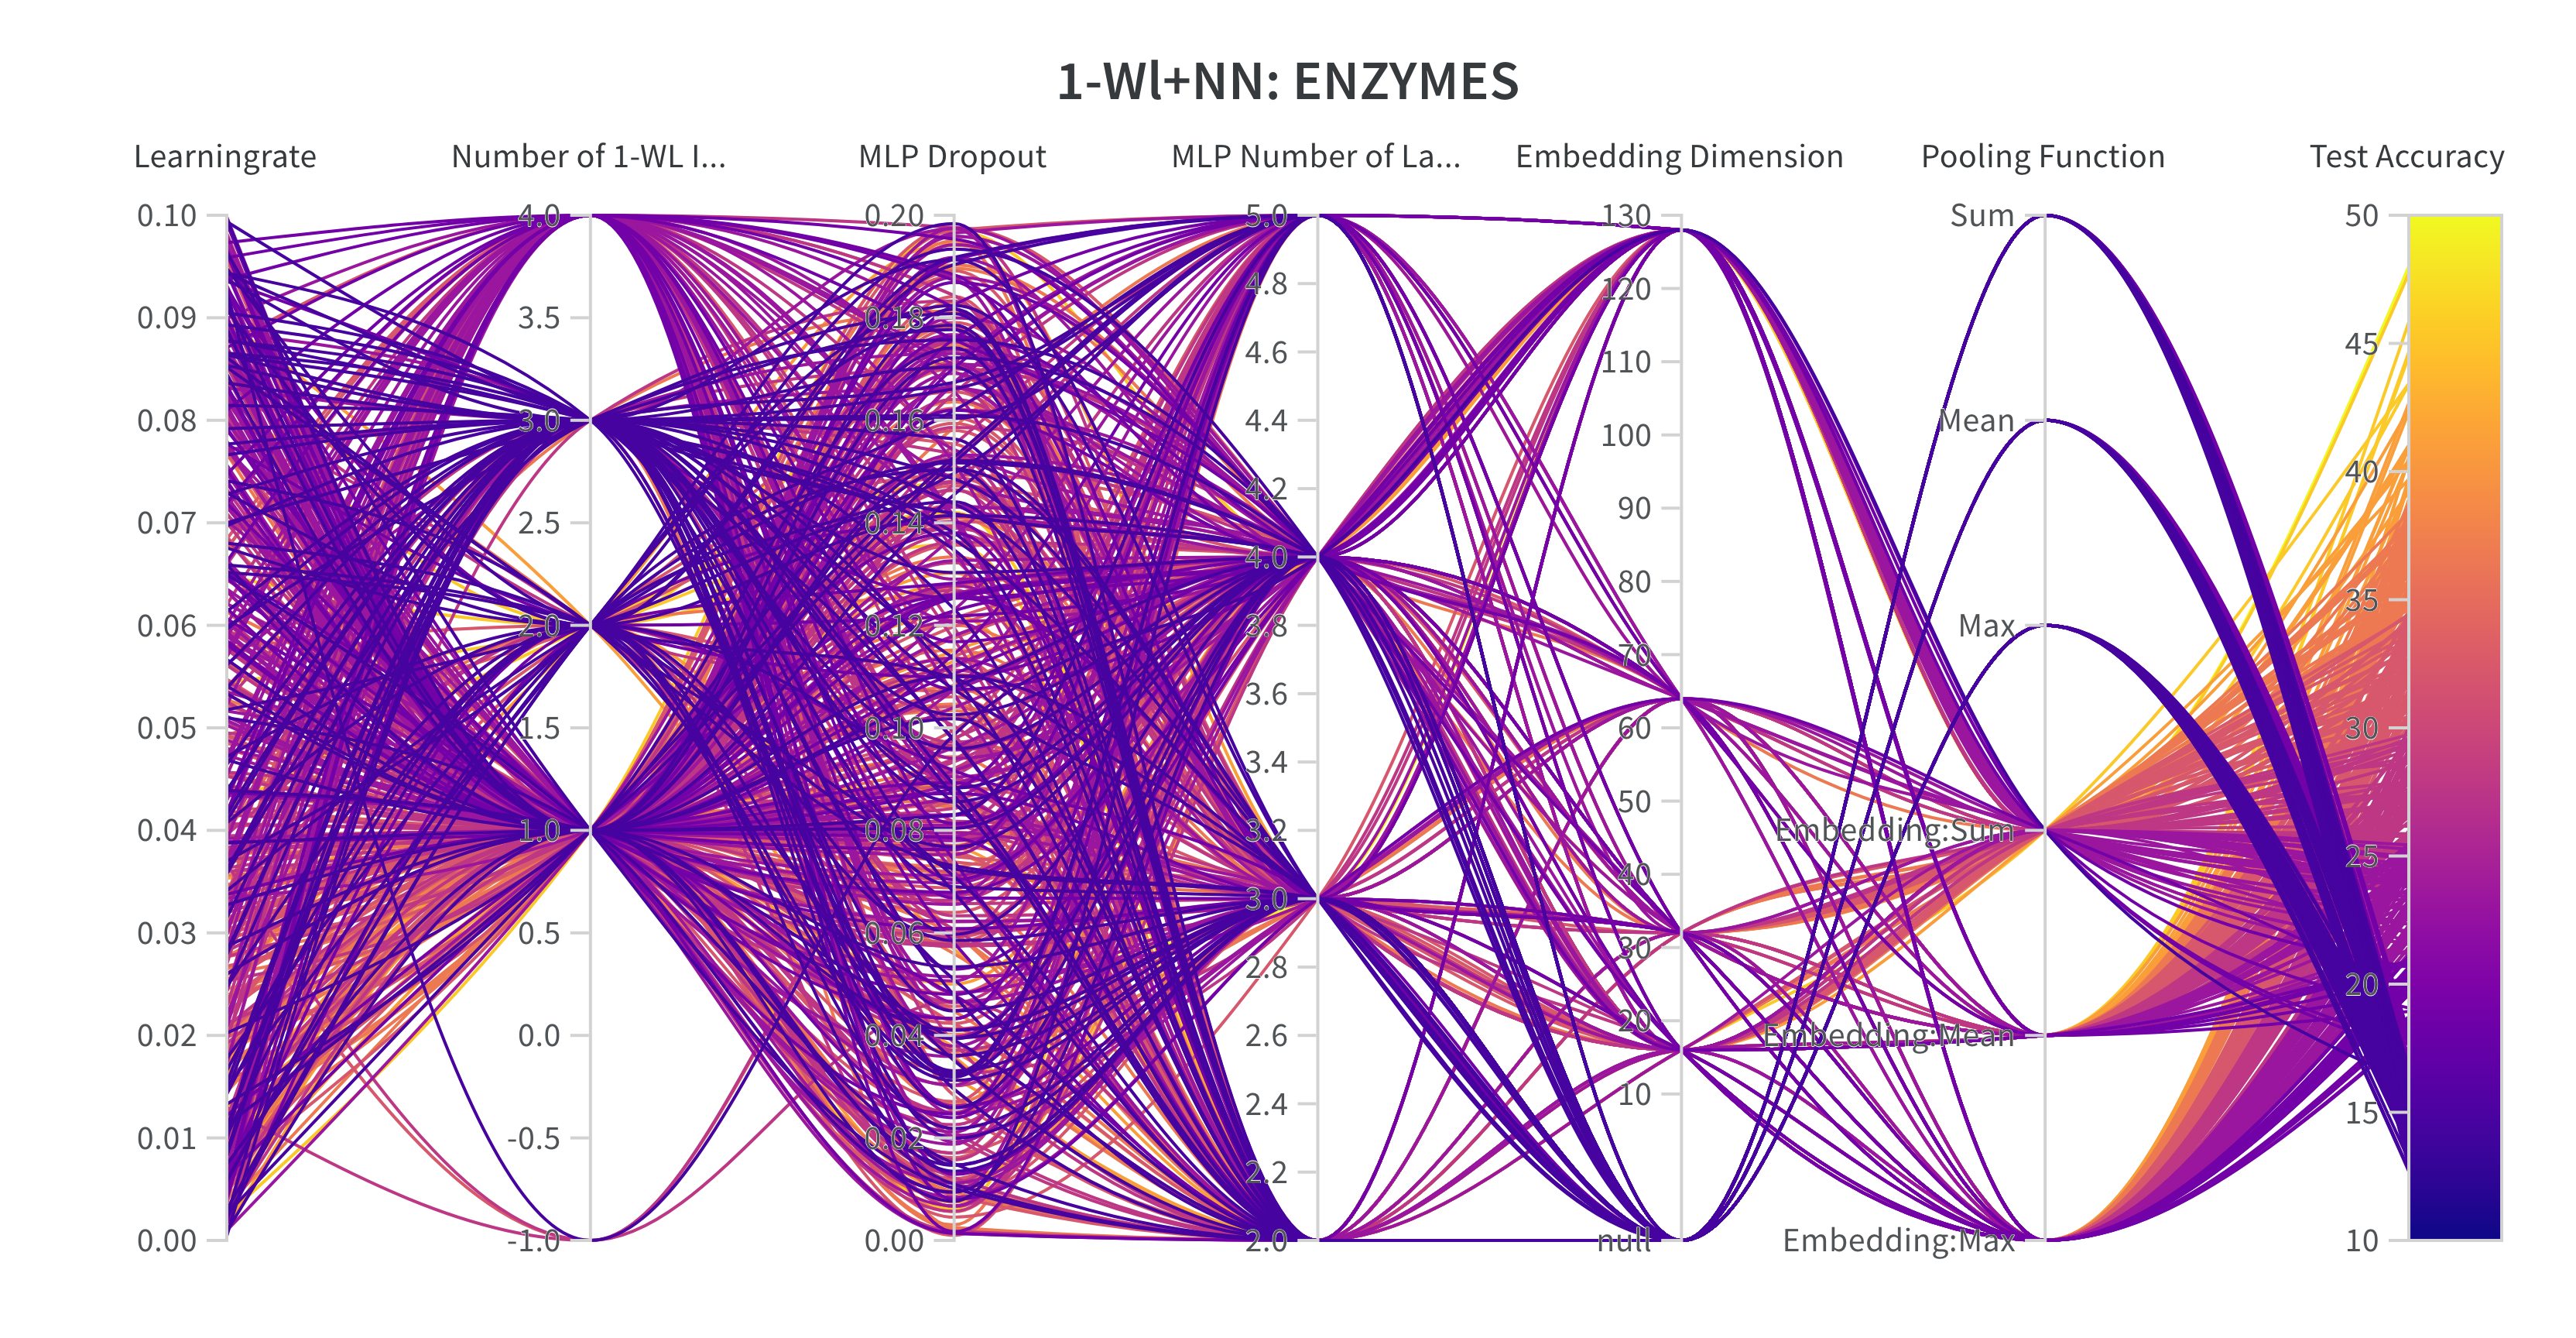
\includegraphics[width=\textwidth, trim={0 75 0 150}, clip]{Figures/hyperparameter_wlnn_enzymes.png}
    \caption{Overview of the effects of each hyperparameter on the accuracy of the corresponding configured \wlnn model for the \enzymes dataset.}
    \label{fig:wandb_wlnn_enzymes}
\end{figure}

\subsubsection{\wlnn Configurations on the IMDB-BINARY Dataset}
\begin{figure}[H]
    \centering
    \includegraphics[width=\textwidth, trim={0 75 0 150}, clip]{Figures/hyperparameter_wlnn_imdb.png}
    \caption{Overview of the effects of each hyperparameter on the accuracy of the corresponding configured \wlnn model for the \imdb dataset.}
    \label{fig:wandb_wlnn_imdb}
\end{figure}
\clearpage

\subsubsection{\wlnn Configurations on the MUTAG Dataset}
\begin{figure}[H]
    \centering
    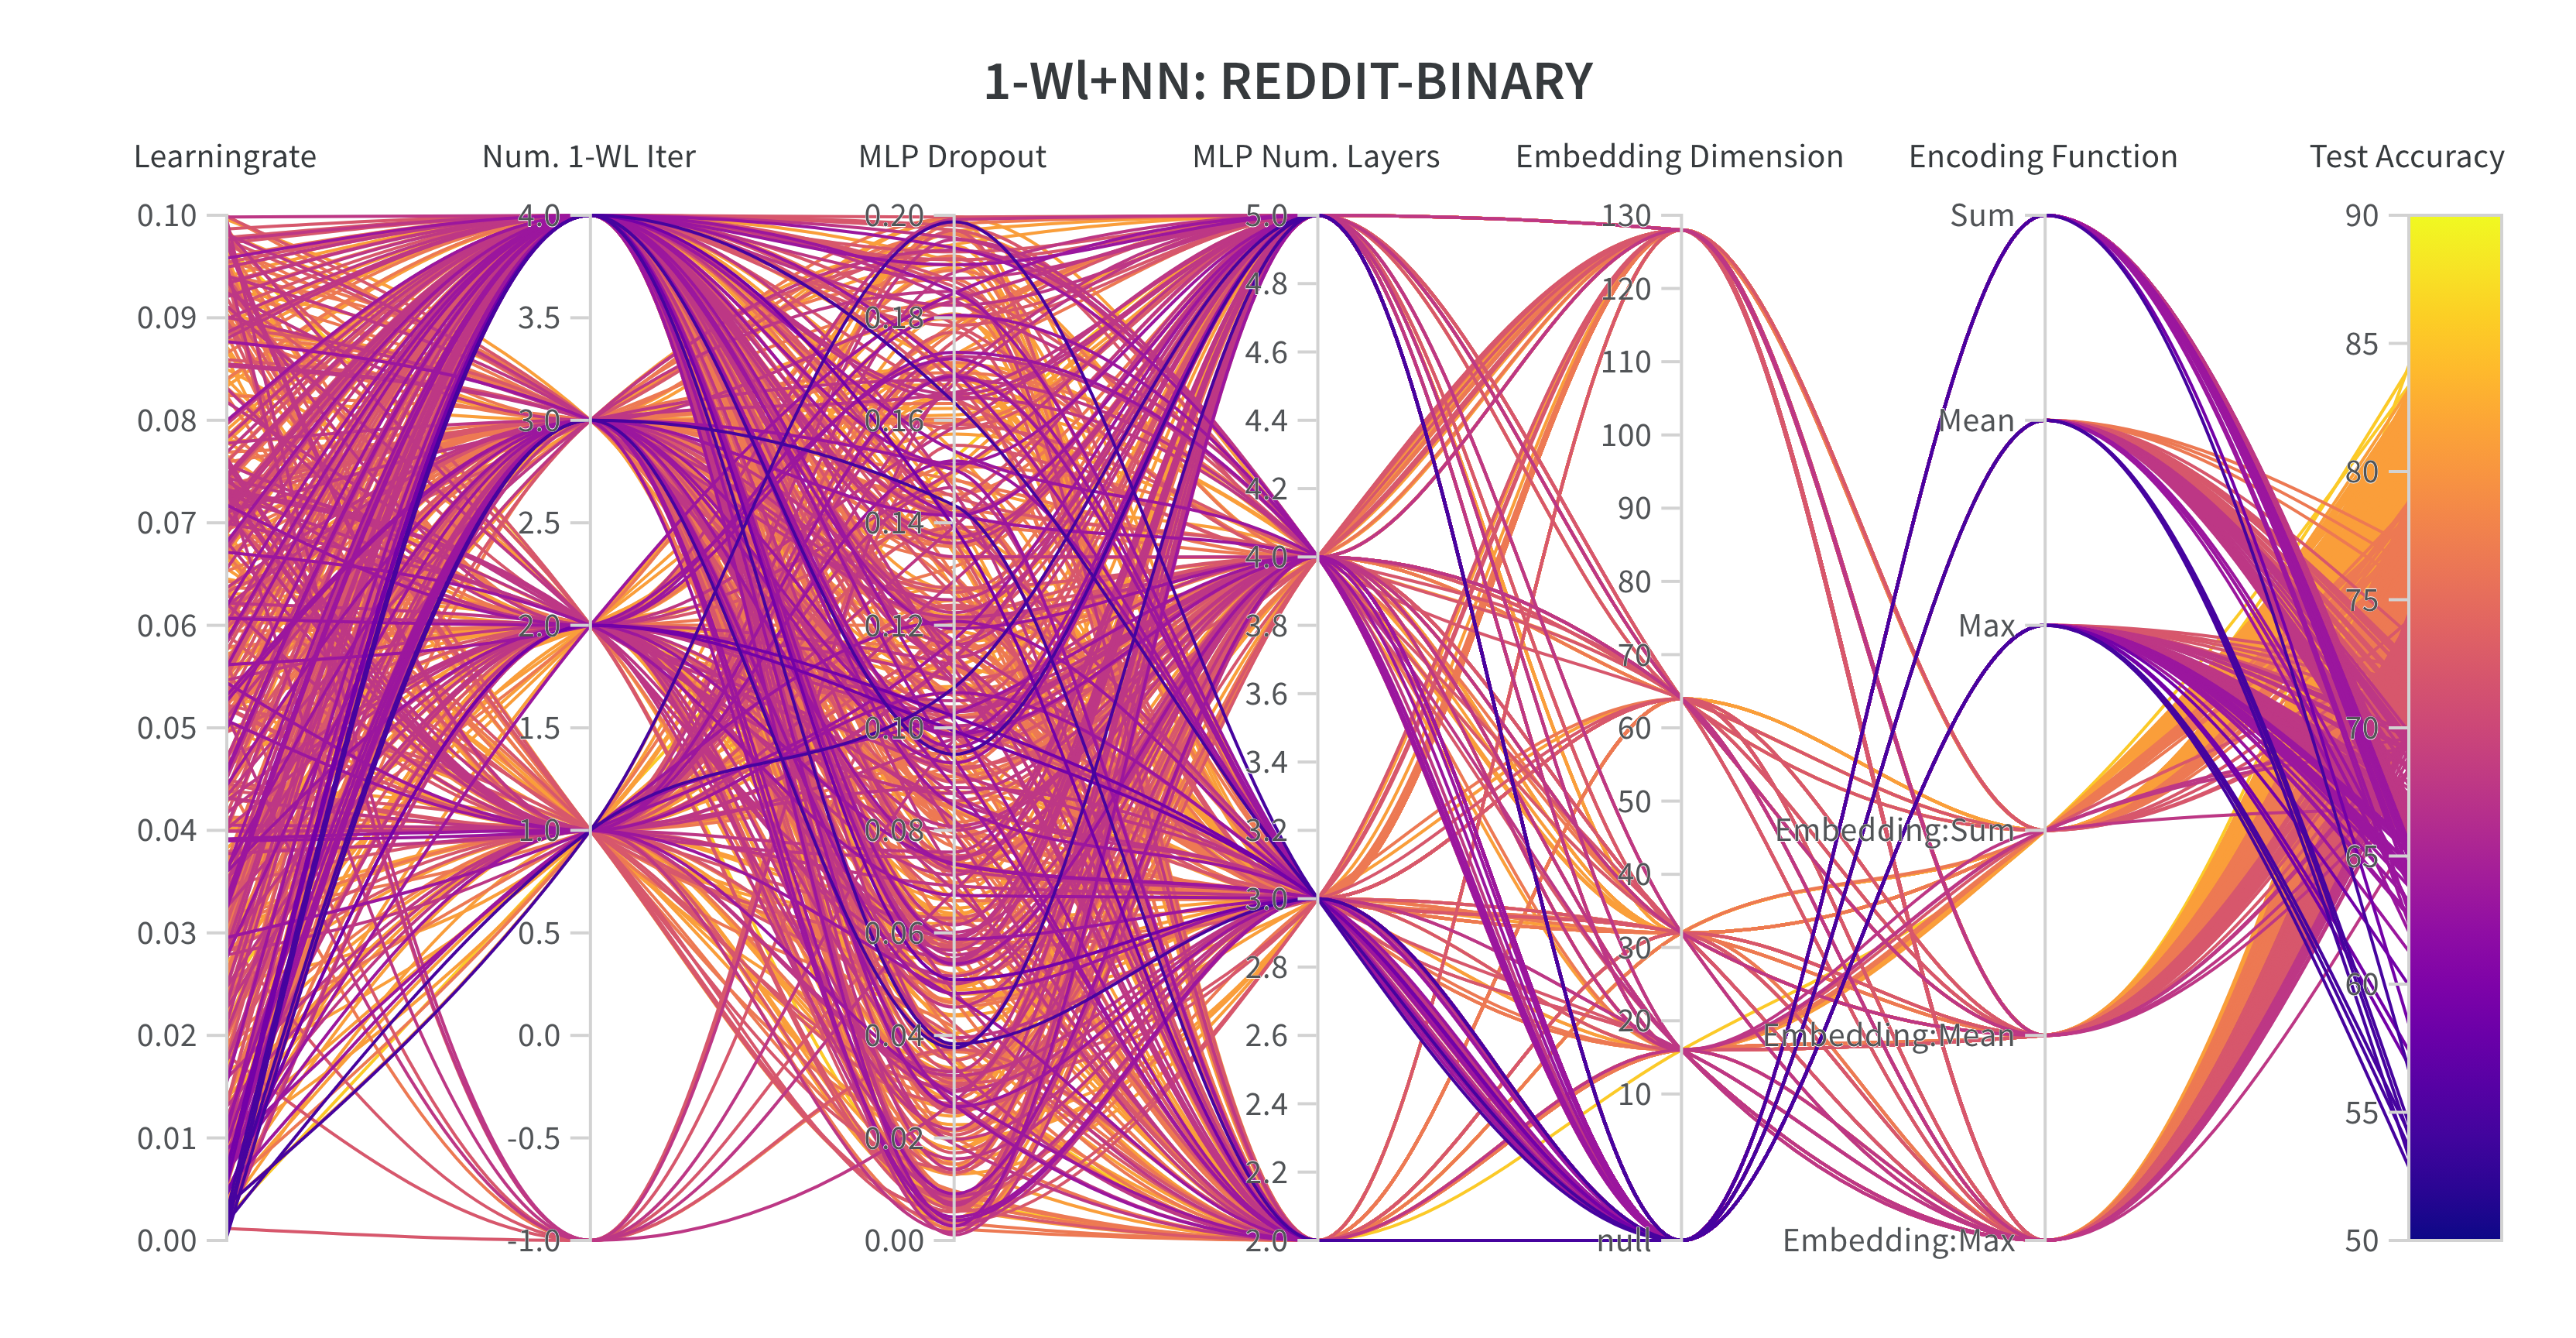
\includegraphics[width=\textwidth, trim={0 75 0 150}, clip]{Figures/hyperparameter_wlnn_mutag.png}
    \caption{Overview of the effects of each hyperparameter on the accuracy of the corresponding configured \wlnn model for the \mutag dataset.}
    \label{fig:wandb_wlnn_mutag}
\end{figure}

\subsubsection{\wlnn Configurations on the NCI1 Dataset}
\begin{figure}[H]
    \centering
    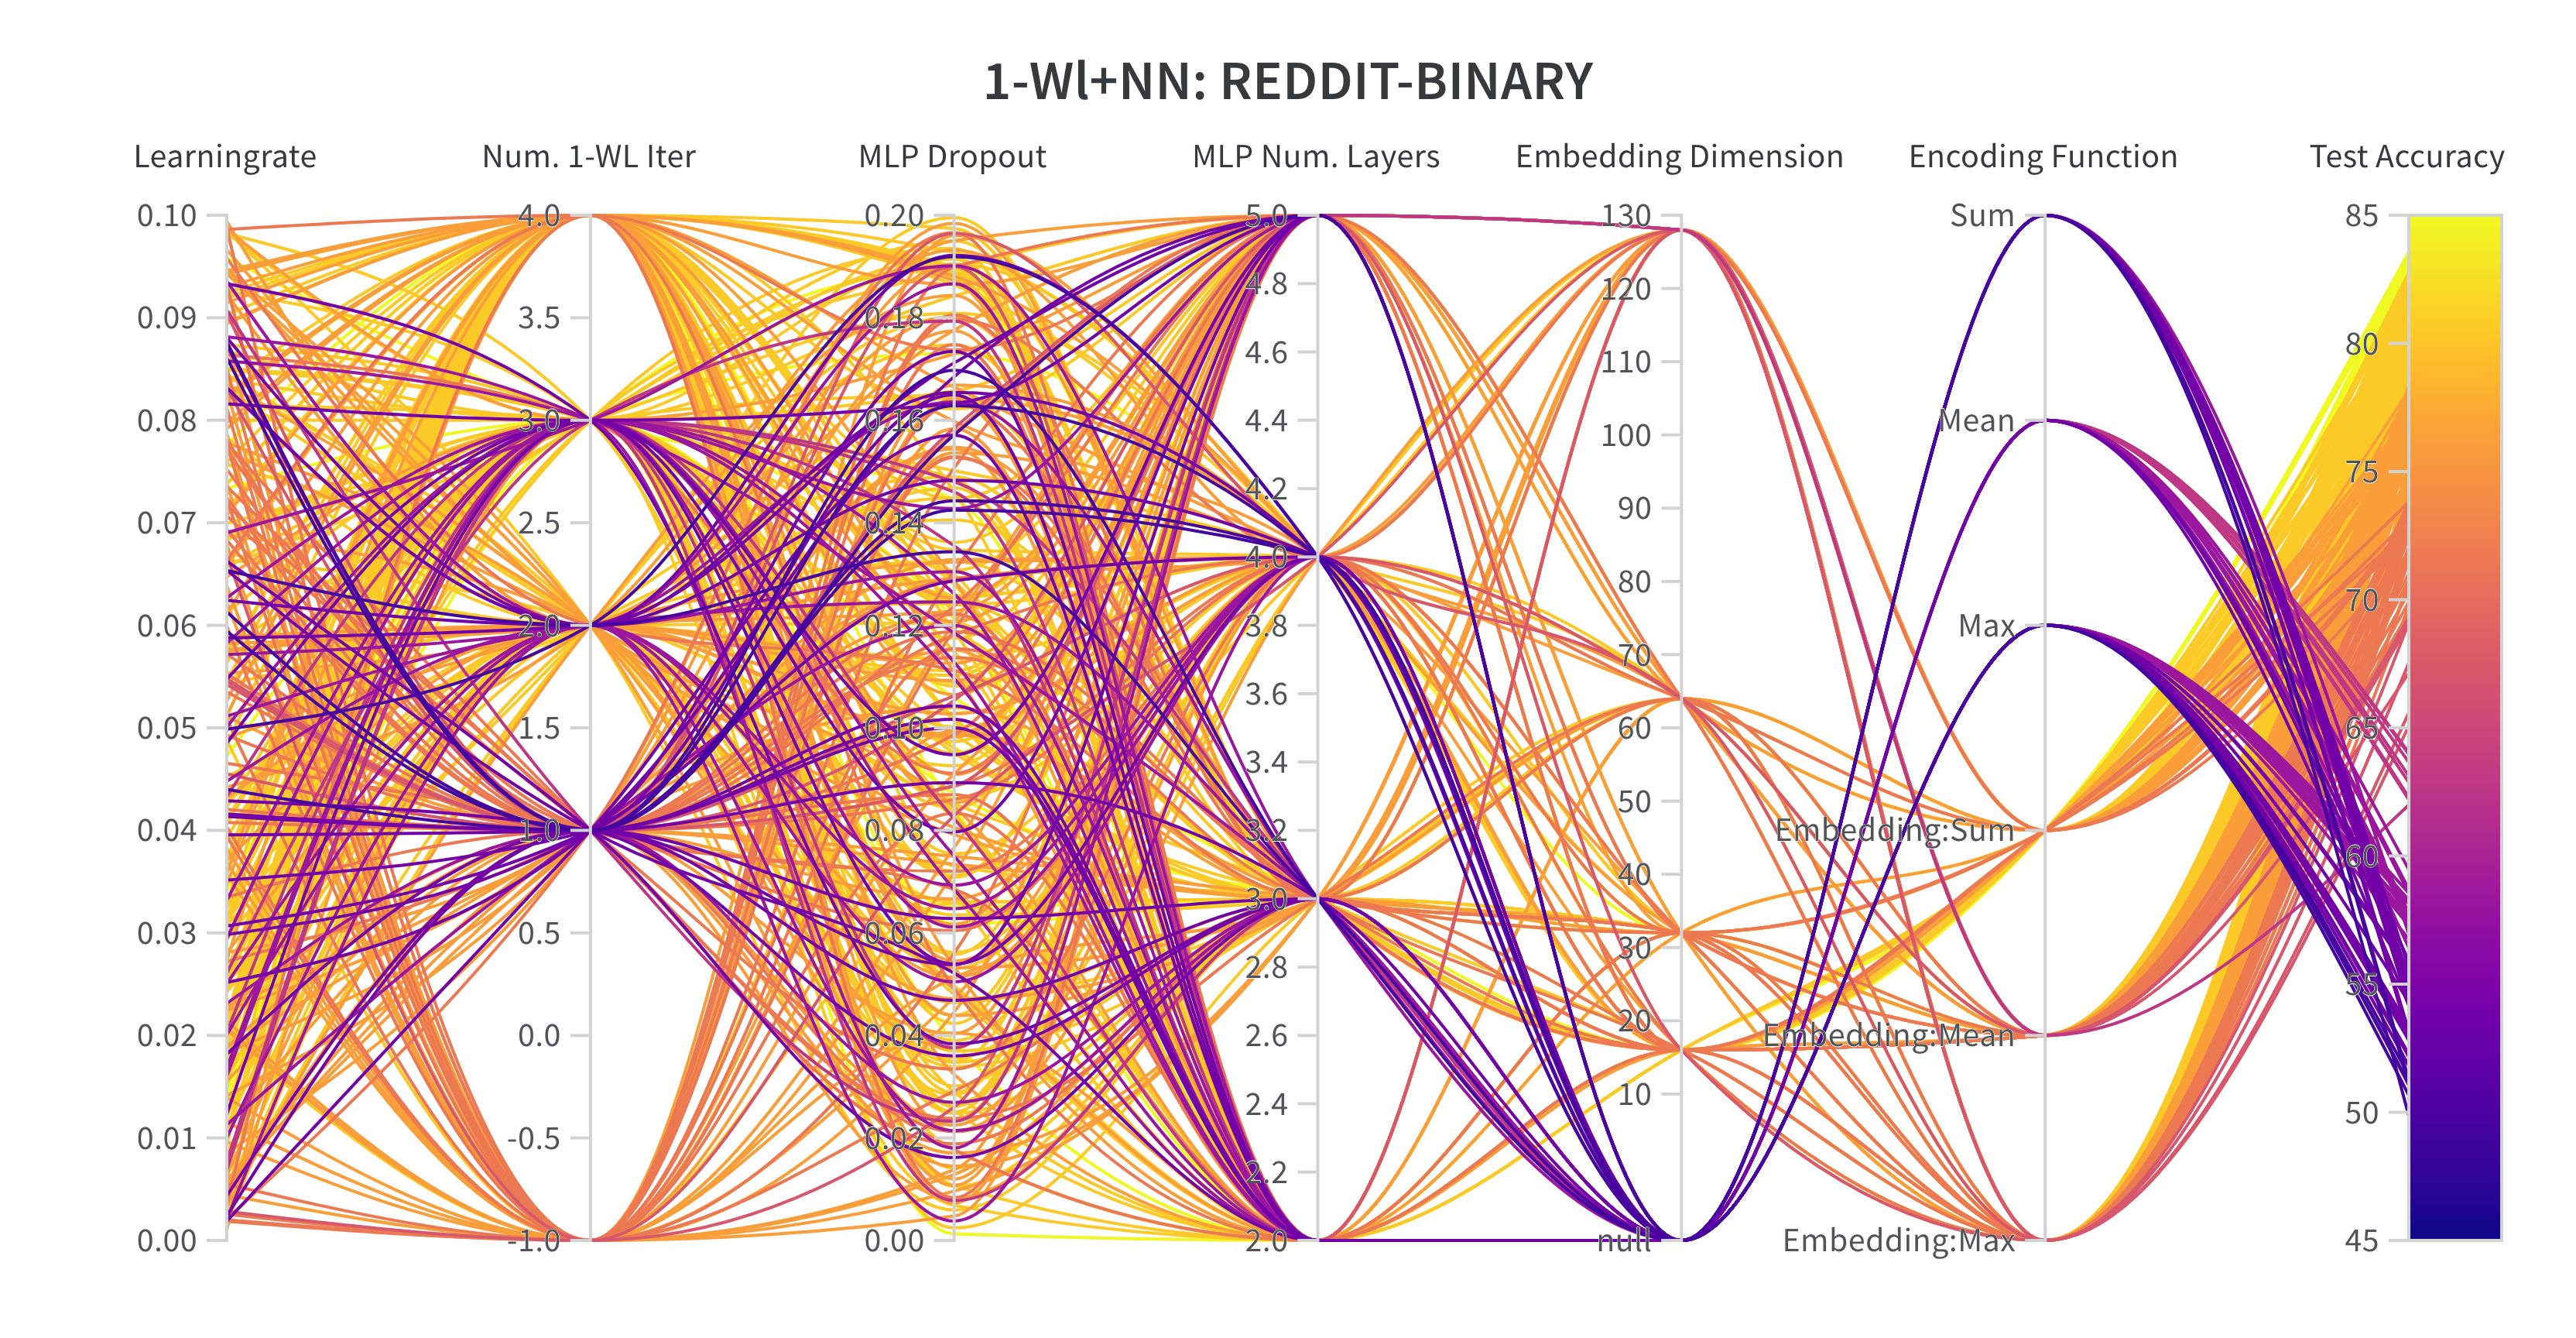
\includegraphics[width=\textwidth, trim={0 75 0 150}, clip]{Figures/hyperparameter_wlnn_nci1.png}
    \caption{Overview of the effects of each hyperparameter on the accuracy of the corresponding configured \wlnn model for the \nci dataset.}
    \label{fig:wandb_wlnn_nci}
\end{figure}
\clearpage

\subsubsection{\wlnn Configurations on the PROTEINS Dataset}
\begin{figure}[H]
    \centering
    \includegraphics[width=\textwidth, trim={0 75 0 150}, clip]{Figures/hyperparameter_wlnn_proteins.png}
    \caption{Overview of the effects of each hyperparameter on the accuracy of the corresponding configured \wlnn model for the \proteins dataset.}
    \label{fig:wandb_wlnn_proteins}
\end{figure}

\subsubsection{\wlnn Configurations on the REDDIT-BINARY Dataset}
\begin{figure}[H]
    \centering
    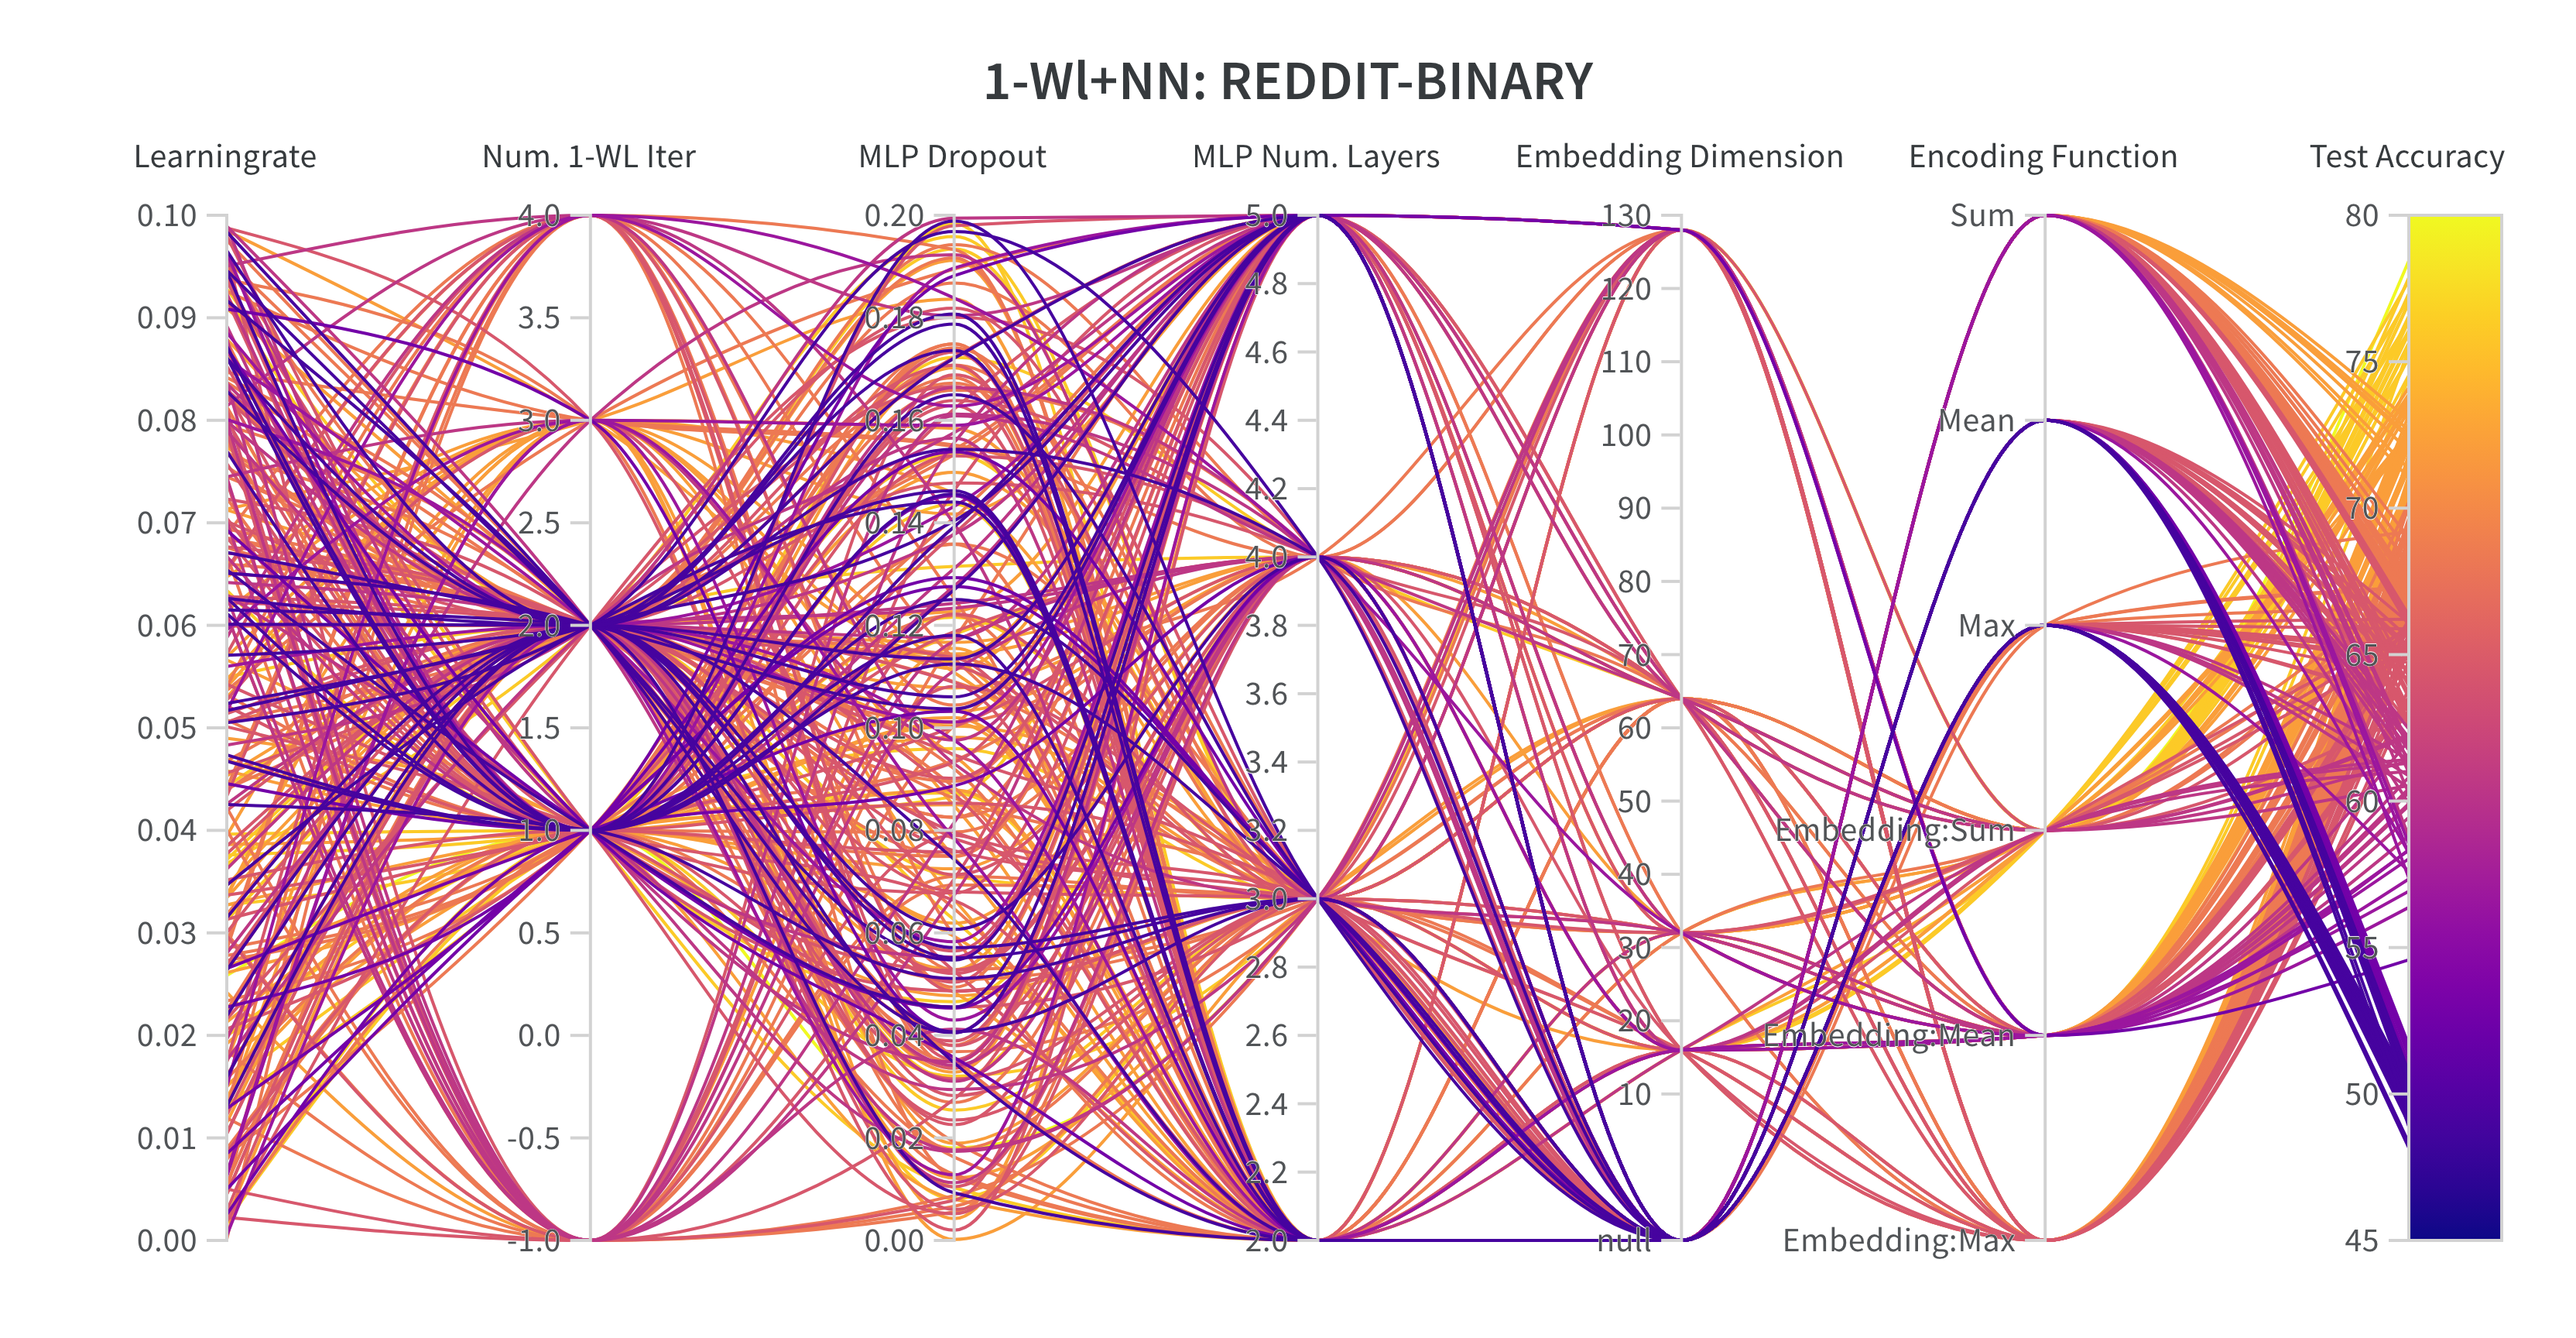
\includegraphics[width=\textwidth, trim={0 75 0 150}, clip]{Figures/hyperparameter_wlnn_reddit.png}
    \caption{Overview of the effects of each hyperparameter on the accuracy of the corresponding configured \wlnn model for the \reddit dataset.}
    \label{fig:wandb_wlnn_reddit}
\end{figure}
\clearpage


\subsection{Impact of each Hyperparameter for \gnns}
In this section, we present the results of our hyperparameter optimization for the \gnn framework on each classification dataset. We will use the same visualization explained and utilized in the previous section, customized to the hyperparameters of the \gnn models.

\subsubsection{\gnn Configurations on the ENZYMES Dataset}
\begin{figure}[H]
    \centering
    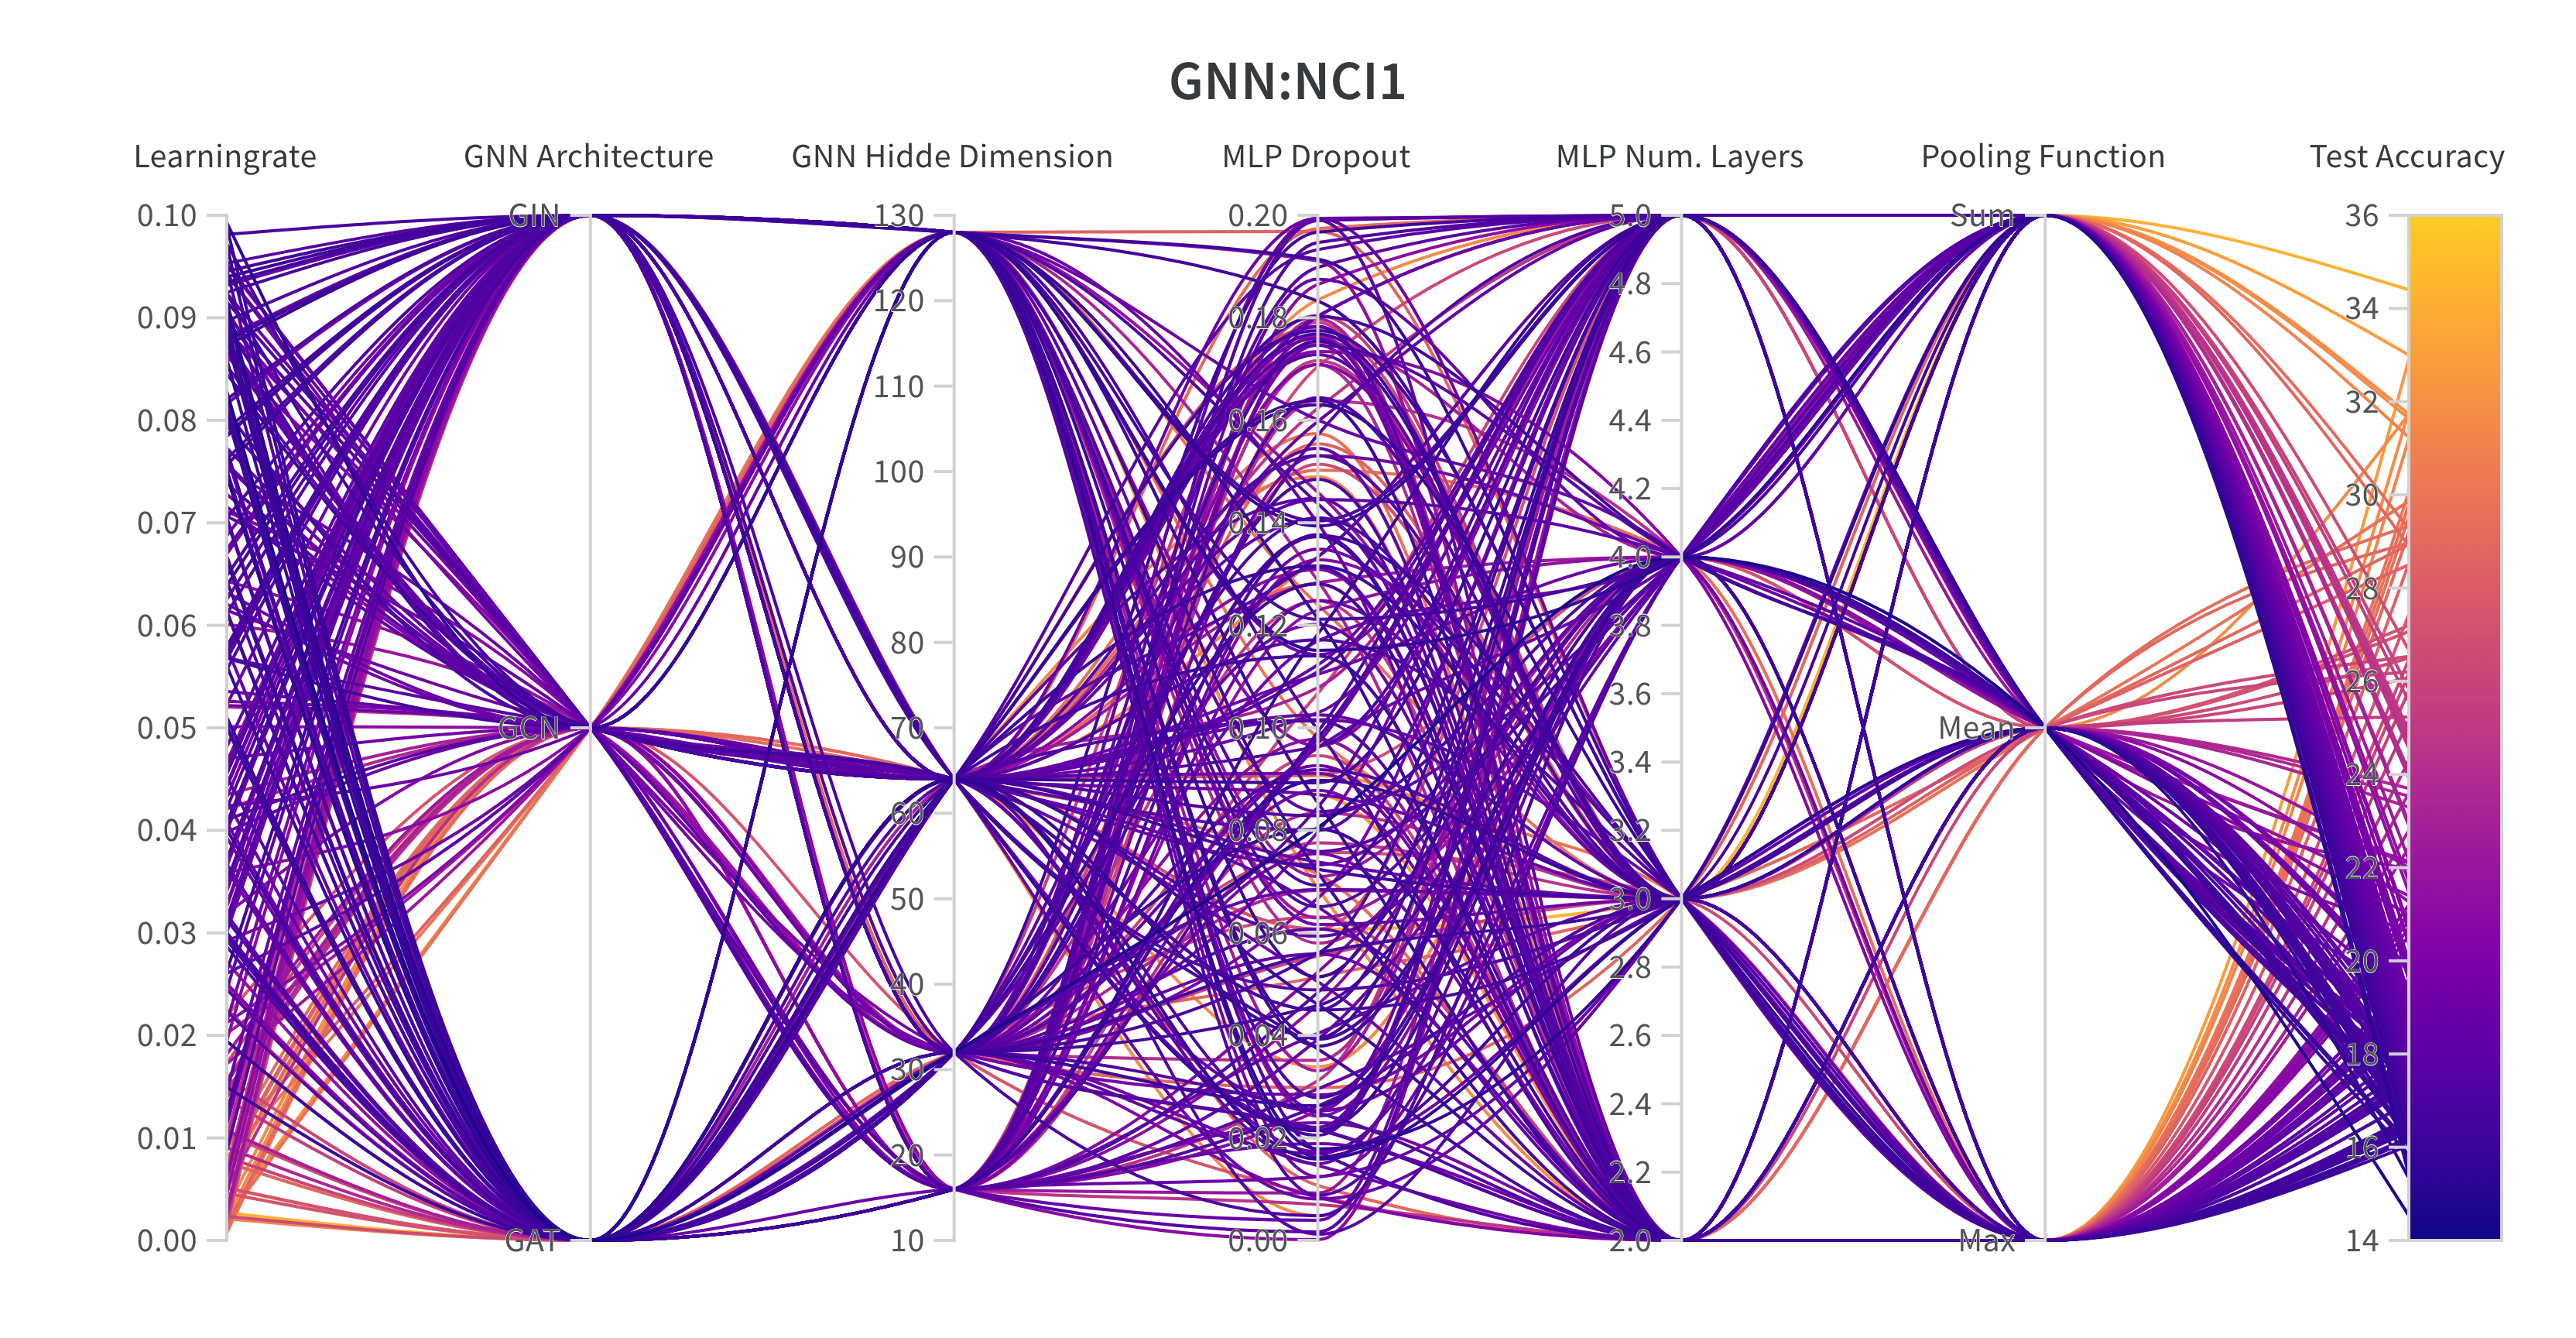
\includegraphics[width=\textwidth, trim={0 75 0 150}, clip]{Figures/hyperparameter_gnn_enzymes.png}
    \caption{Overview of the effects of each hyperparameter on the accuracy of the corresponding configured \gnn model for the \enzymes dataset.}
    \label{fig:wandb_gnn_enzymes}
\end{figure}

\subsubsection{\gnn Configurations on the IMDB-BINARY Dataset}
\begin{figure}[H]
    \centering
    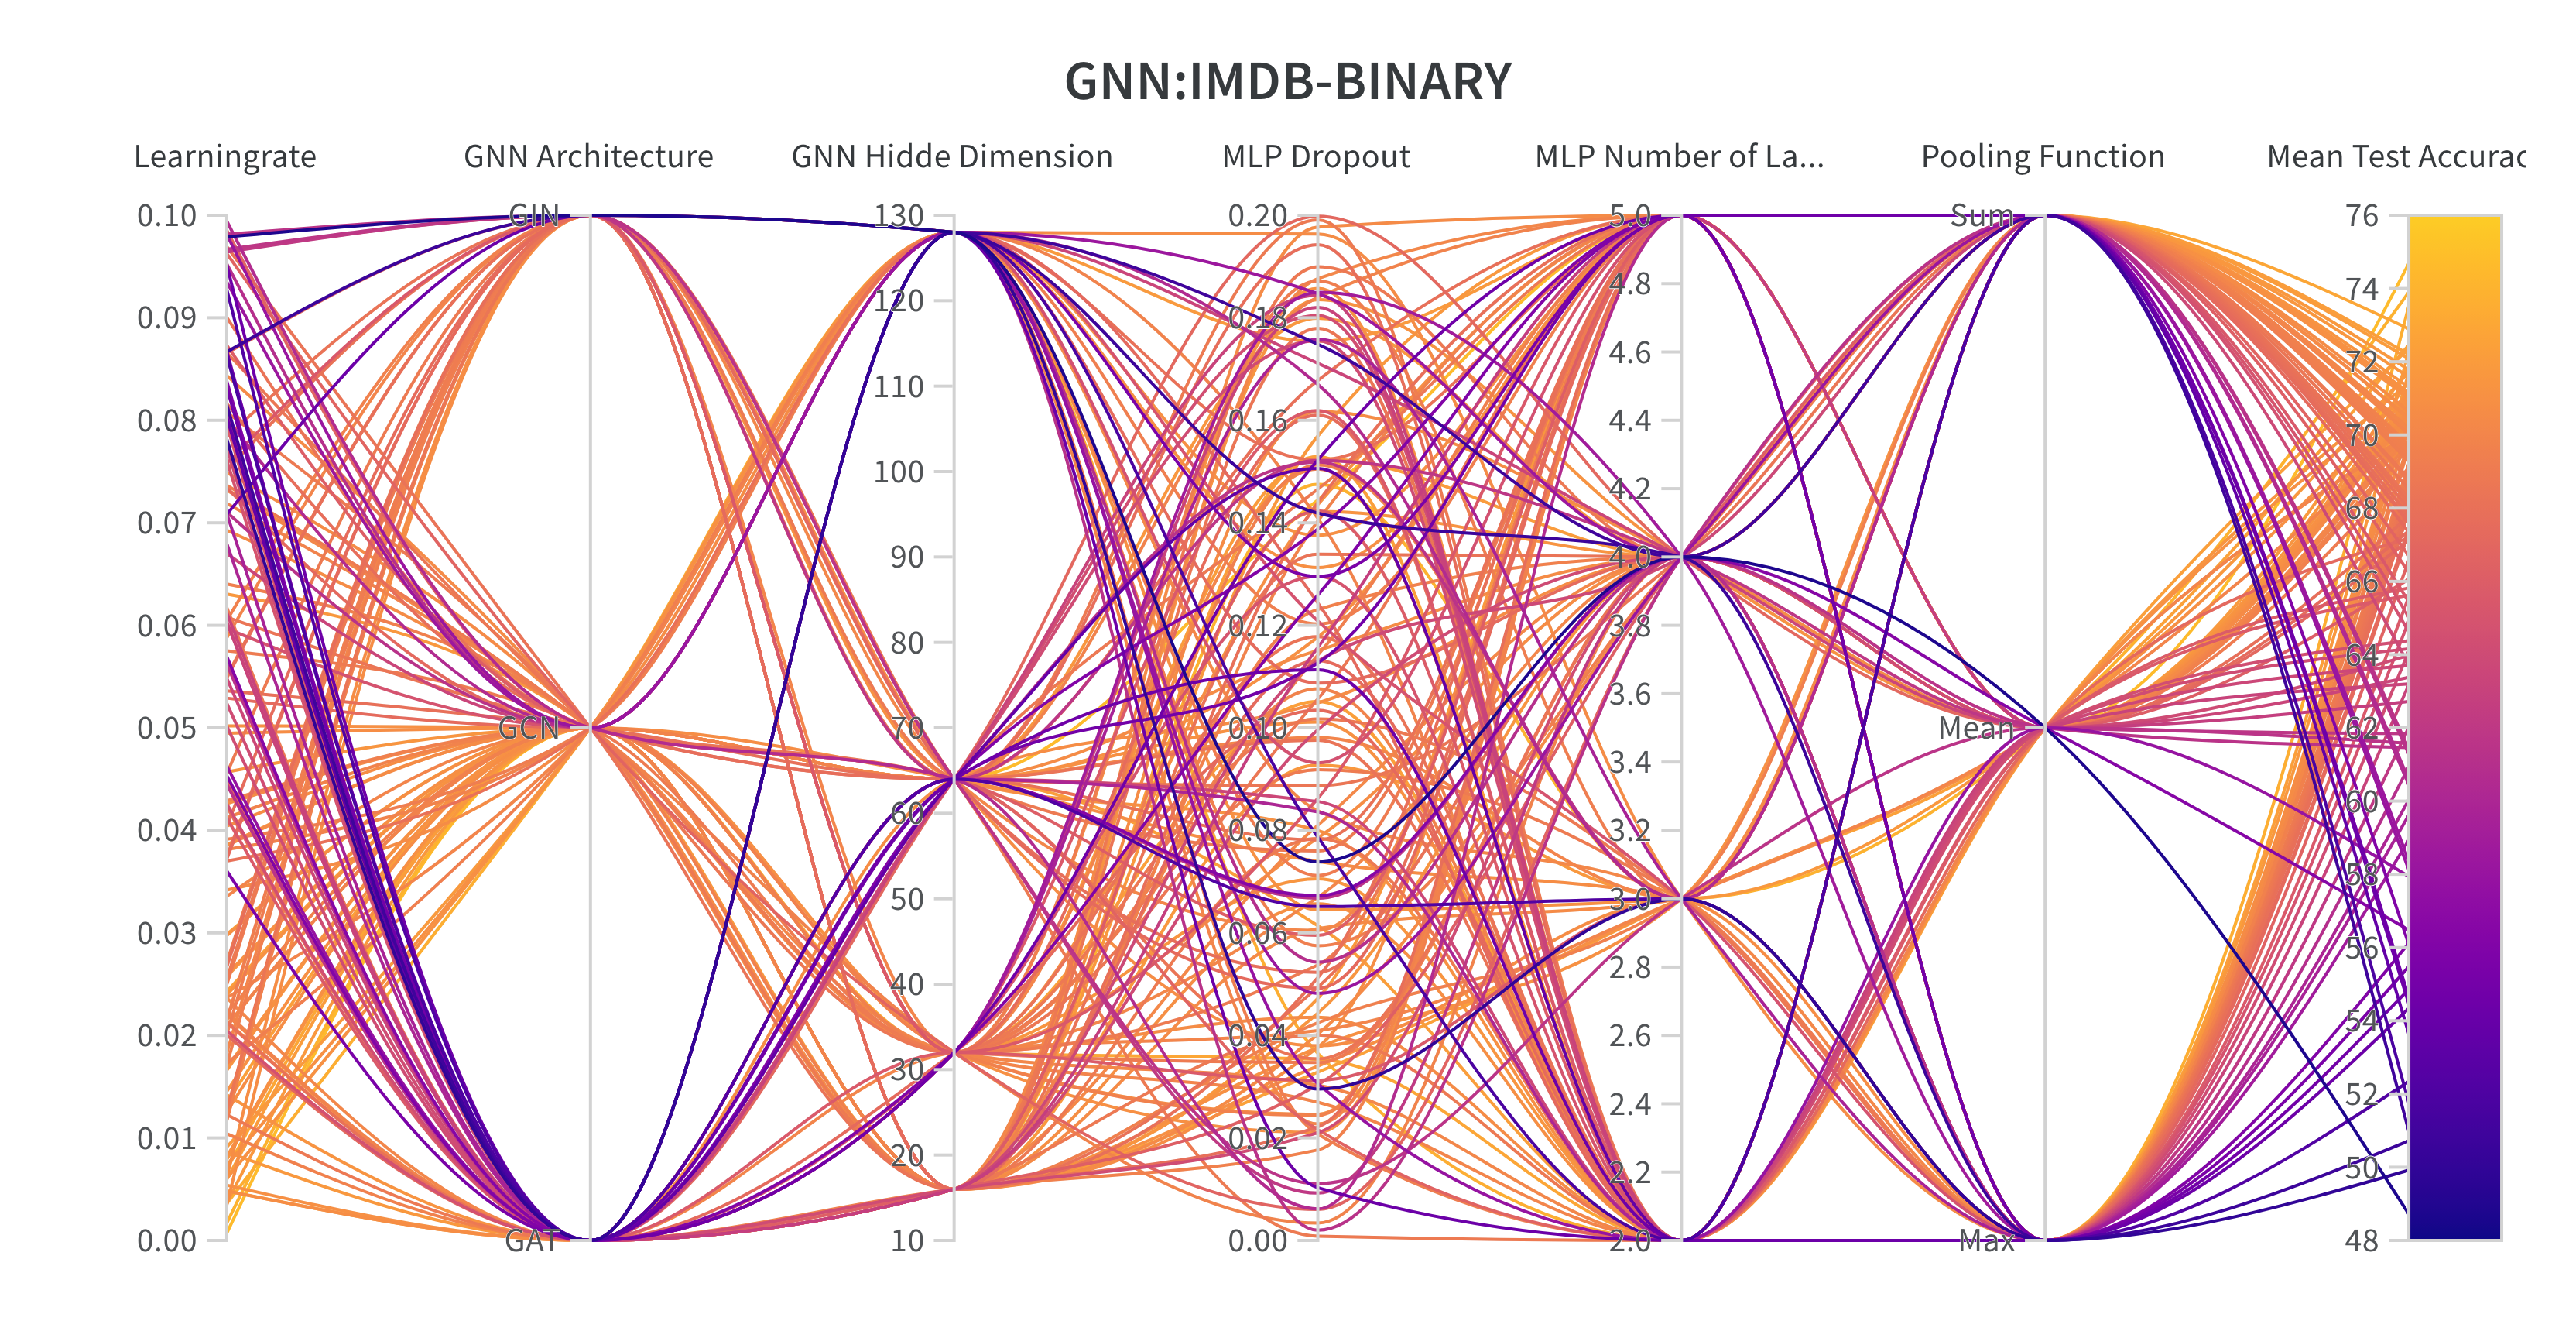
\includegraphics[width=\textwidth, trim={0 75 0 150}, clip]{Figures/hyperparameter_gnn_imdb.png}
    \caption{Overview of the effects of each hyperparameter on the accuracy of the corresponding configured \gnn model for the \imdb dataset.}
    \label{fig:wandb_gnn_imdb}
\end{figure}
\clearpage

\subsubsection{\gnn Configurations on the MUTAG Dataset}
\begin{figure}[H]
    \centering
    \includegraphics[width=\textwidth, trim={0 75 0 150}, clip]{Figures/hyperparameter_gnn_mutag.png}
    \caption{Overview of the effects of each hyperparameter on the accuracy of the corresponding configured \gnn model for the \mutag dataset.}
    \label{fig:wandb_gnn_mutag}
\end{figure}

\subsubsection{\gnn Configurations on the NCI1 Dataset}
\begin{figure}[H]
    \centering
    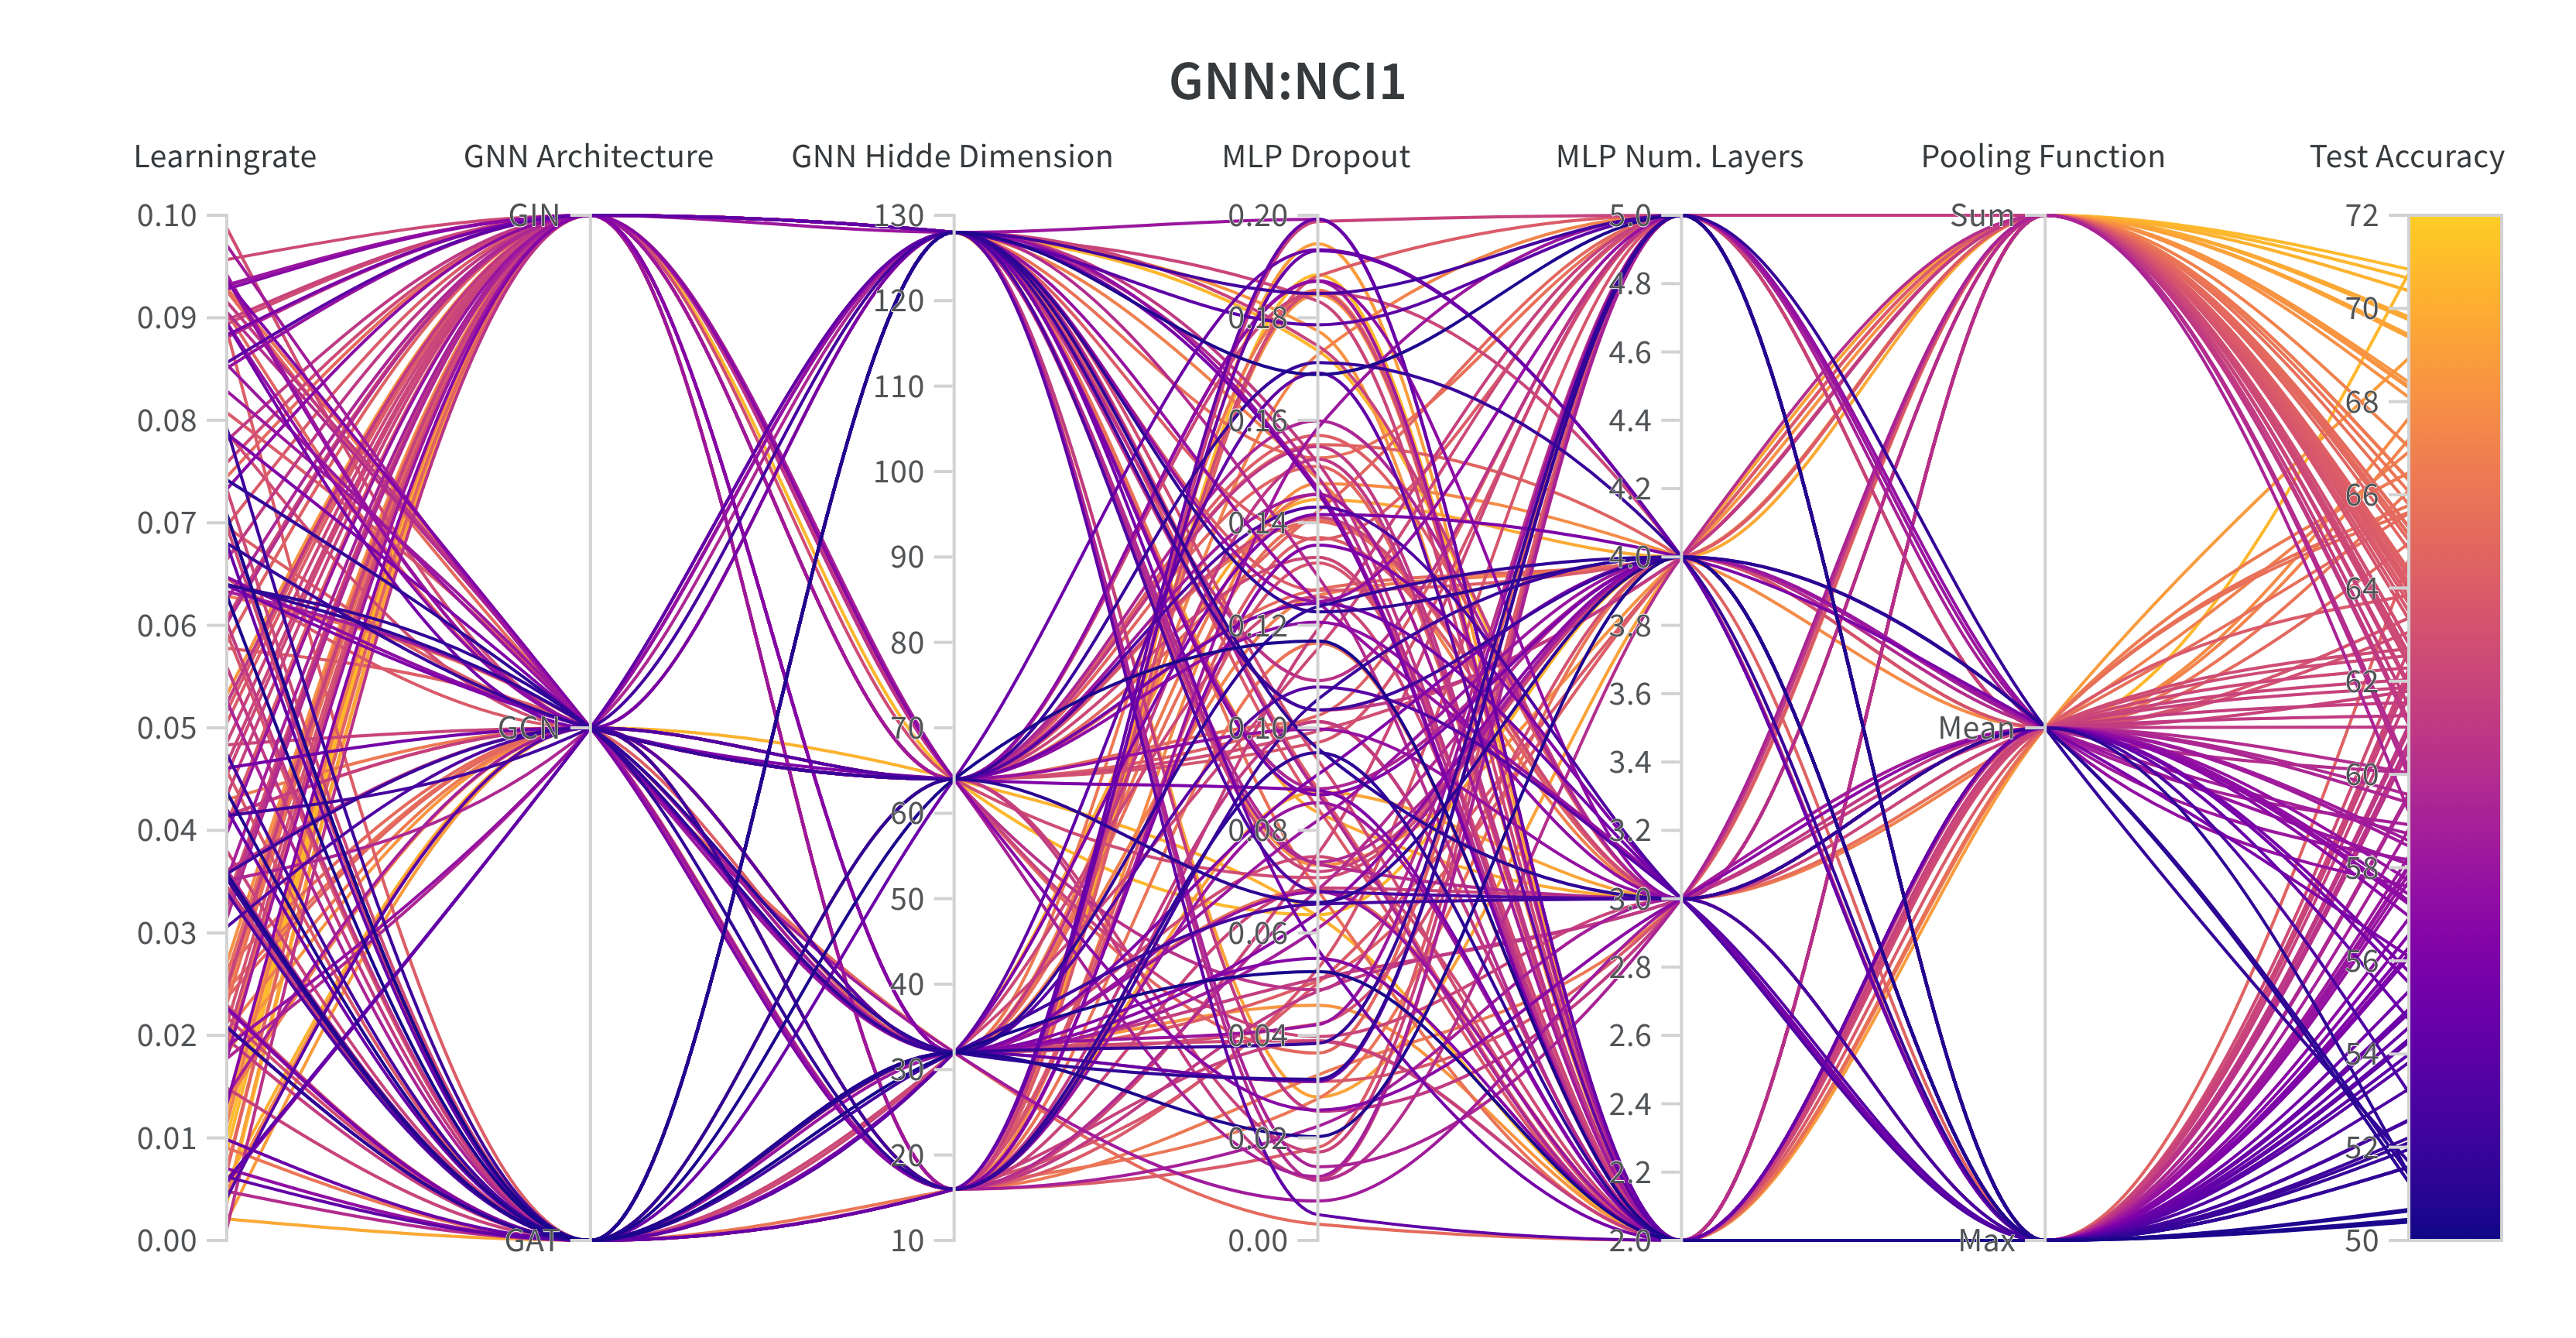
\includegraphics[width=\textwidth, trim={0 75 0 150}, clip]{Figures/hyperparameter_gnn_nci1.png}
    \caption{Overview of the effects of each hyperparameter on the accuracy of the corresponding configured \gnn model for the \nci dataset.}
    \label{fig:wandb_gnn_nci}
\end{figure}
\clearpage

\subsubsection{\gnn Configurations on the PROTEINS Dataset}
\begin{figure}[H]
    \centering
    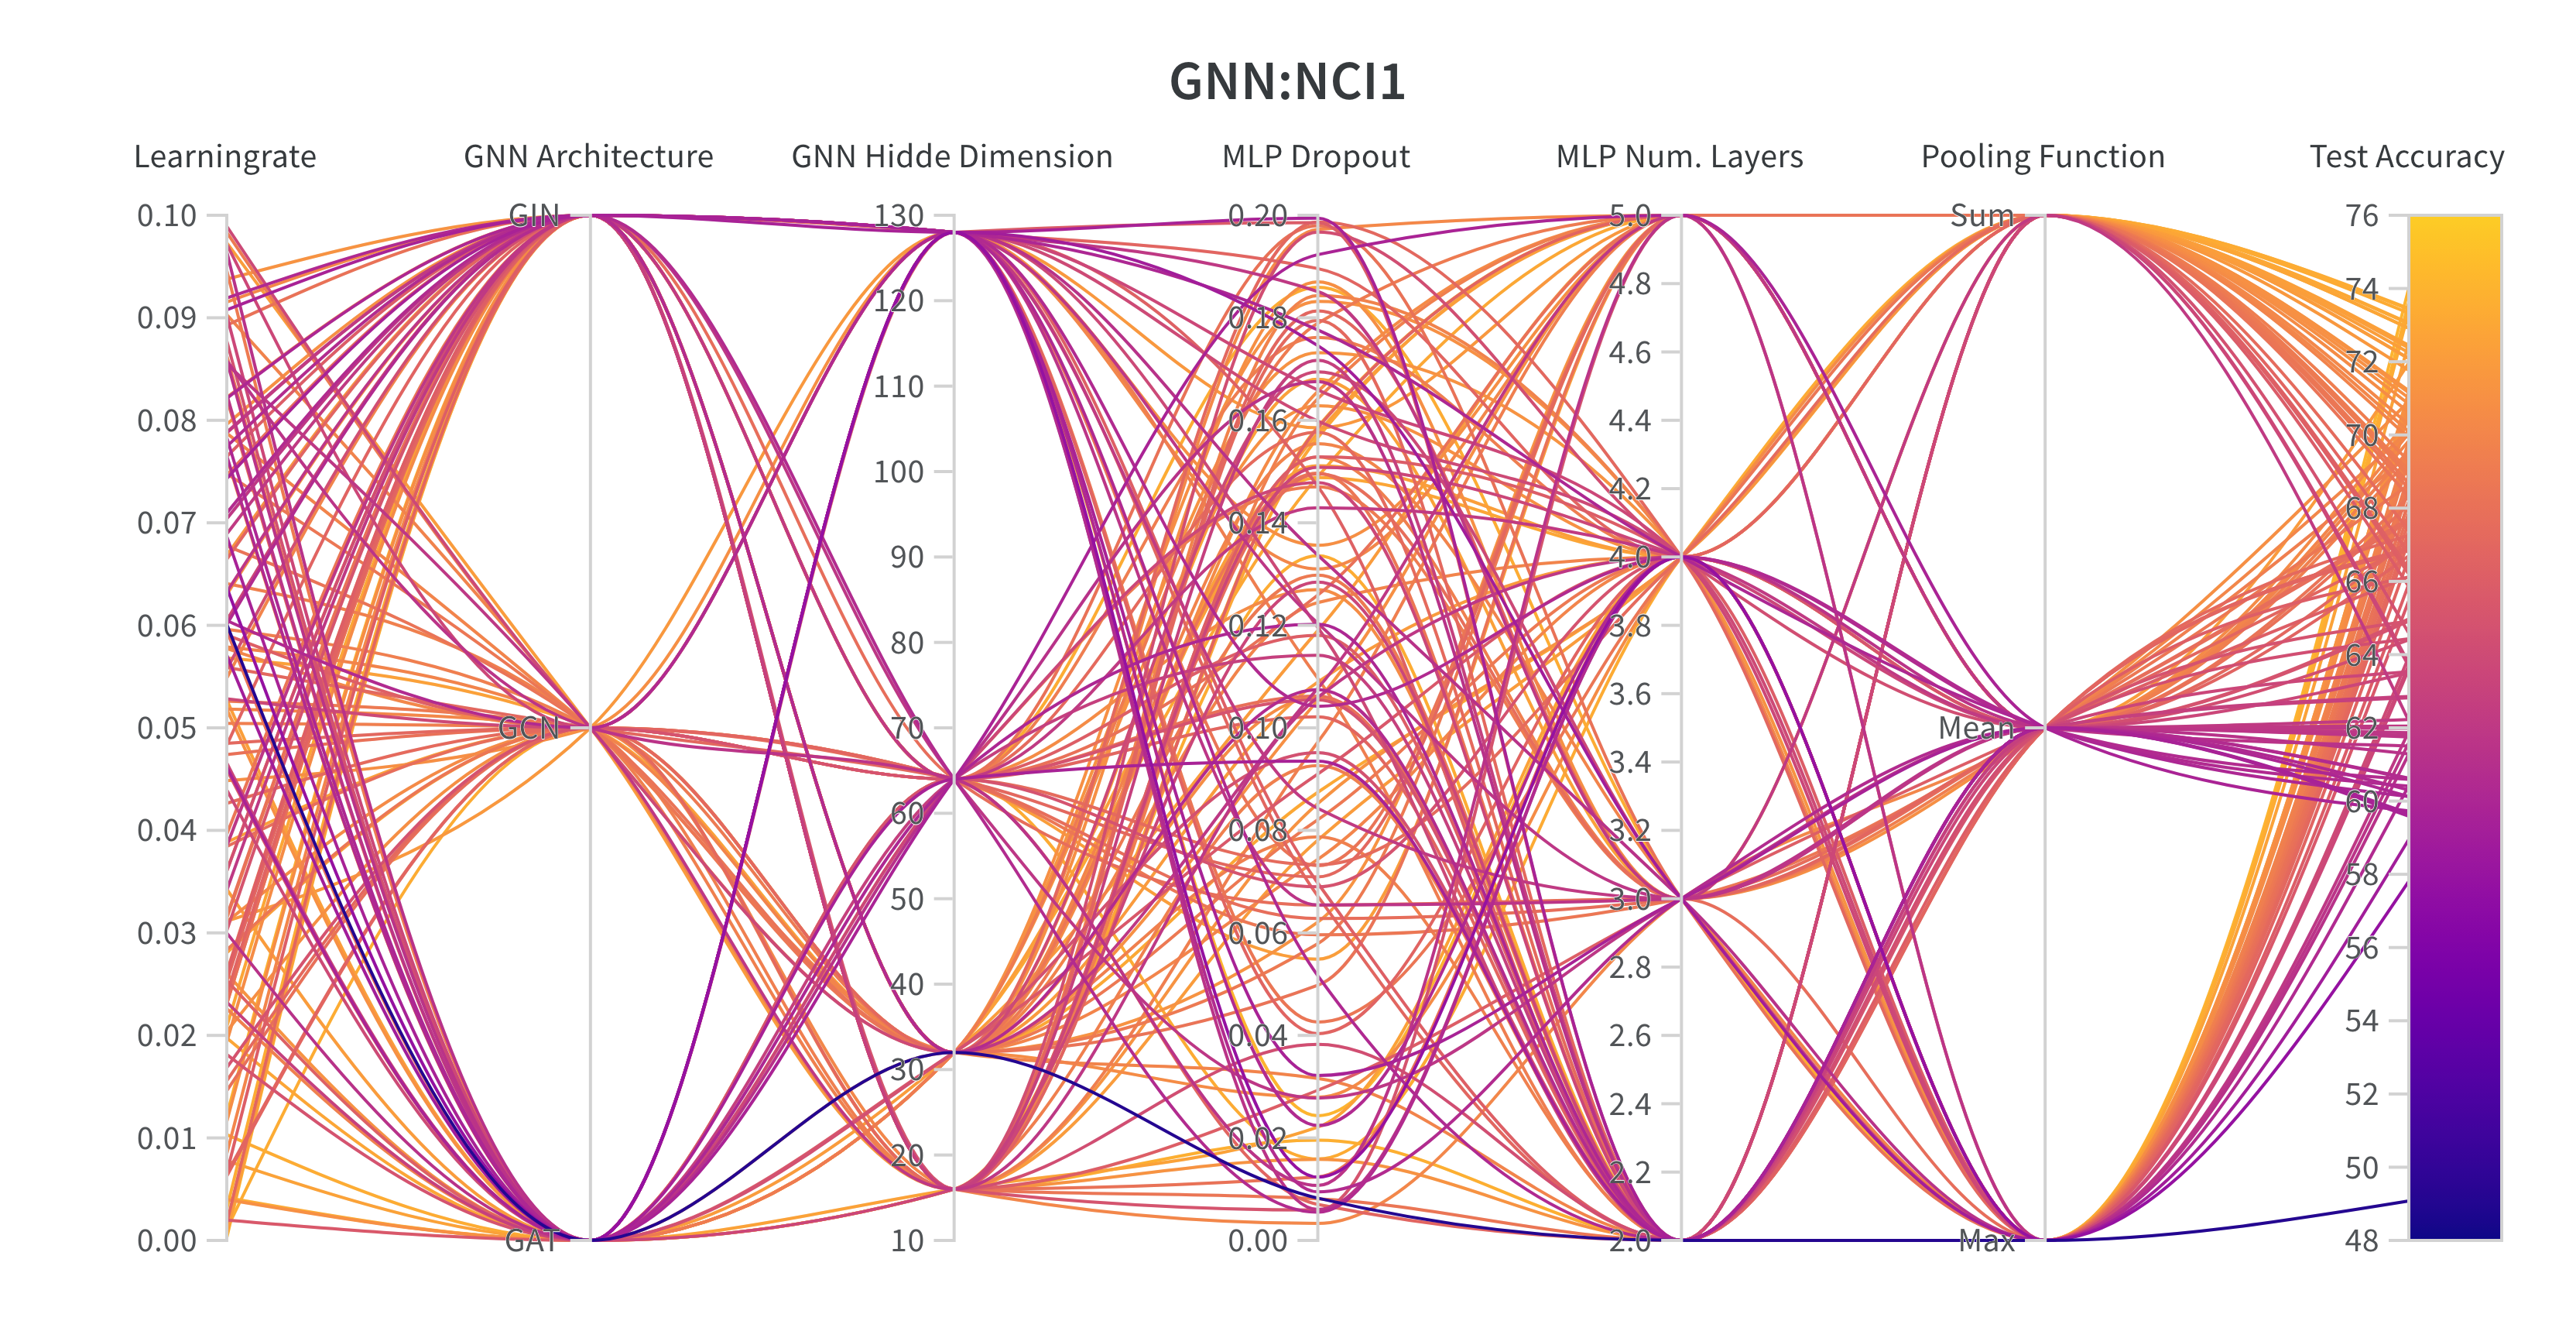
\includegraphics[width=\textwidth, trim={0 75 0 150}, clip]{Figures/hyperparameter_gnn_proteins.png}
    \caption{Overview of the effects of each hyperparameter on the accuracy of the corresponding configured \gnn model for the \proteins dataset.}
    \label{fig:wandb_gnn_proteins}
\end{figure}

\subsubsection{\gnn Configurations on the REDDIT-BINARY Dataset}
\begin{figure}[H]
    \centering
    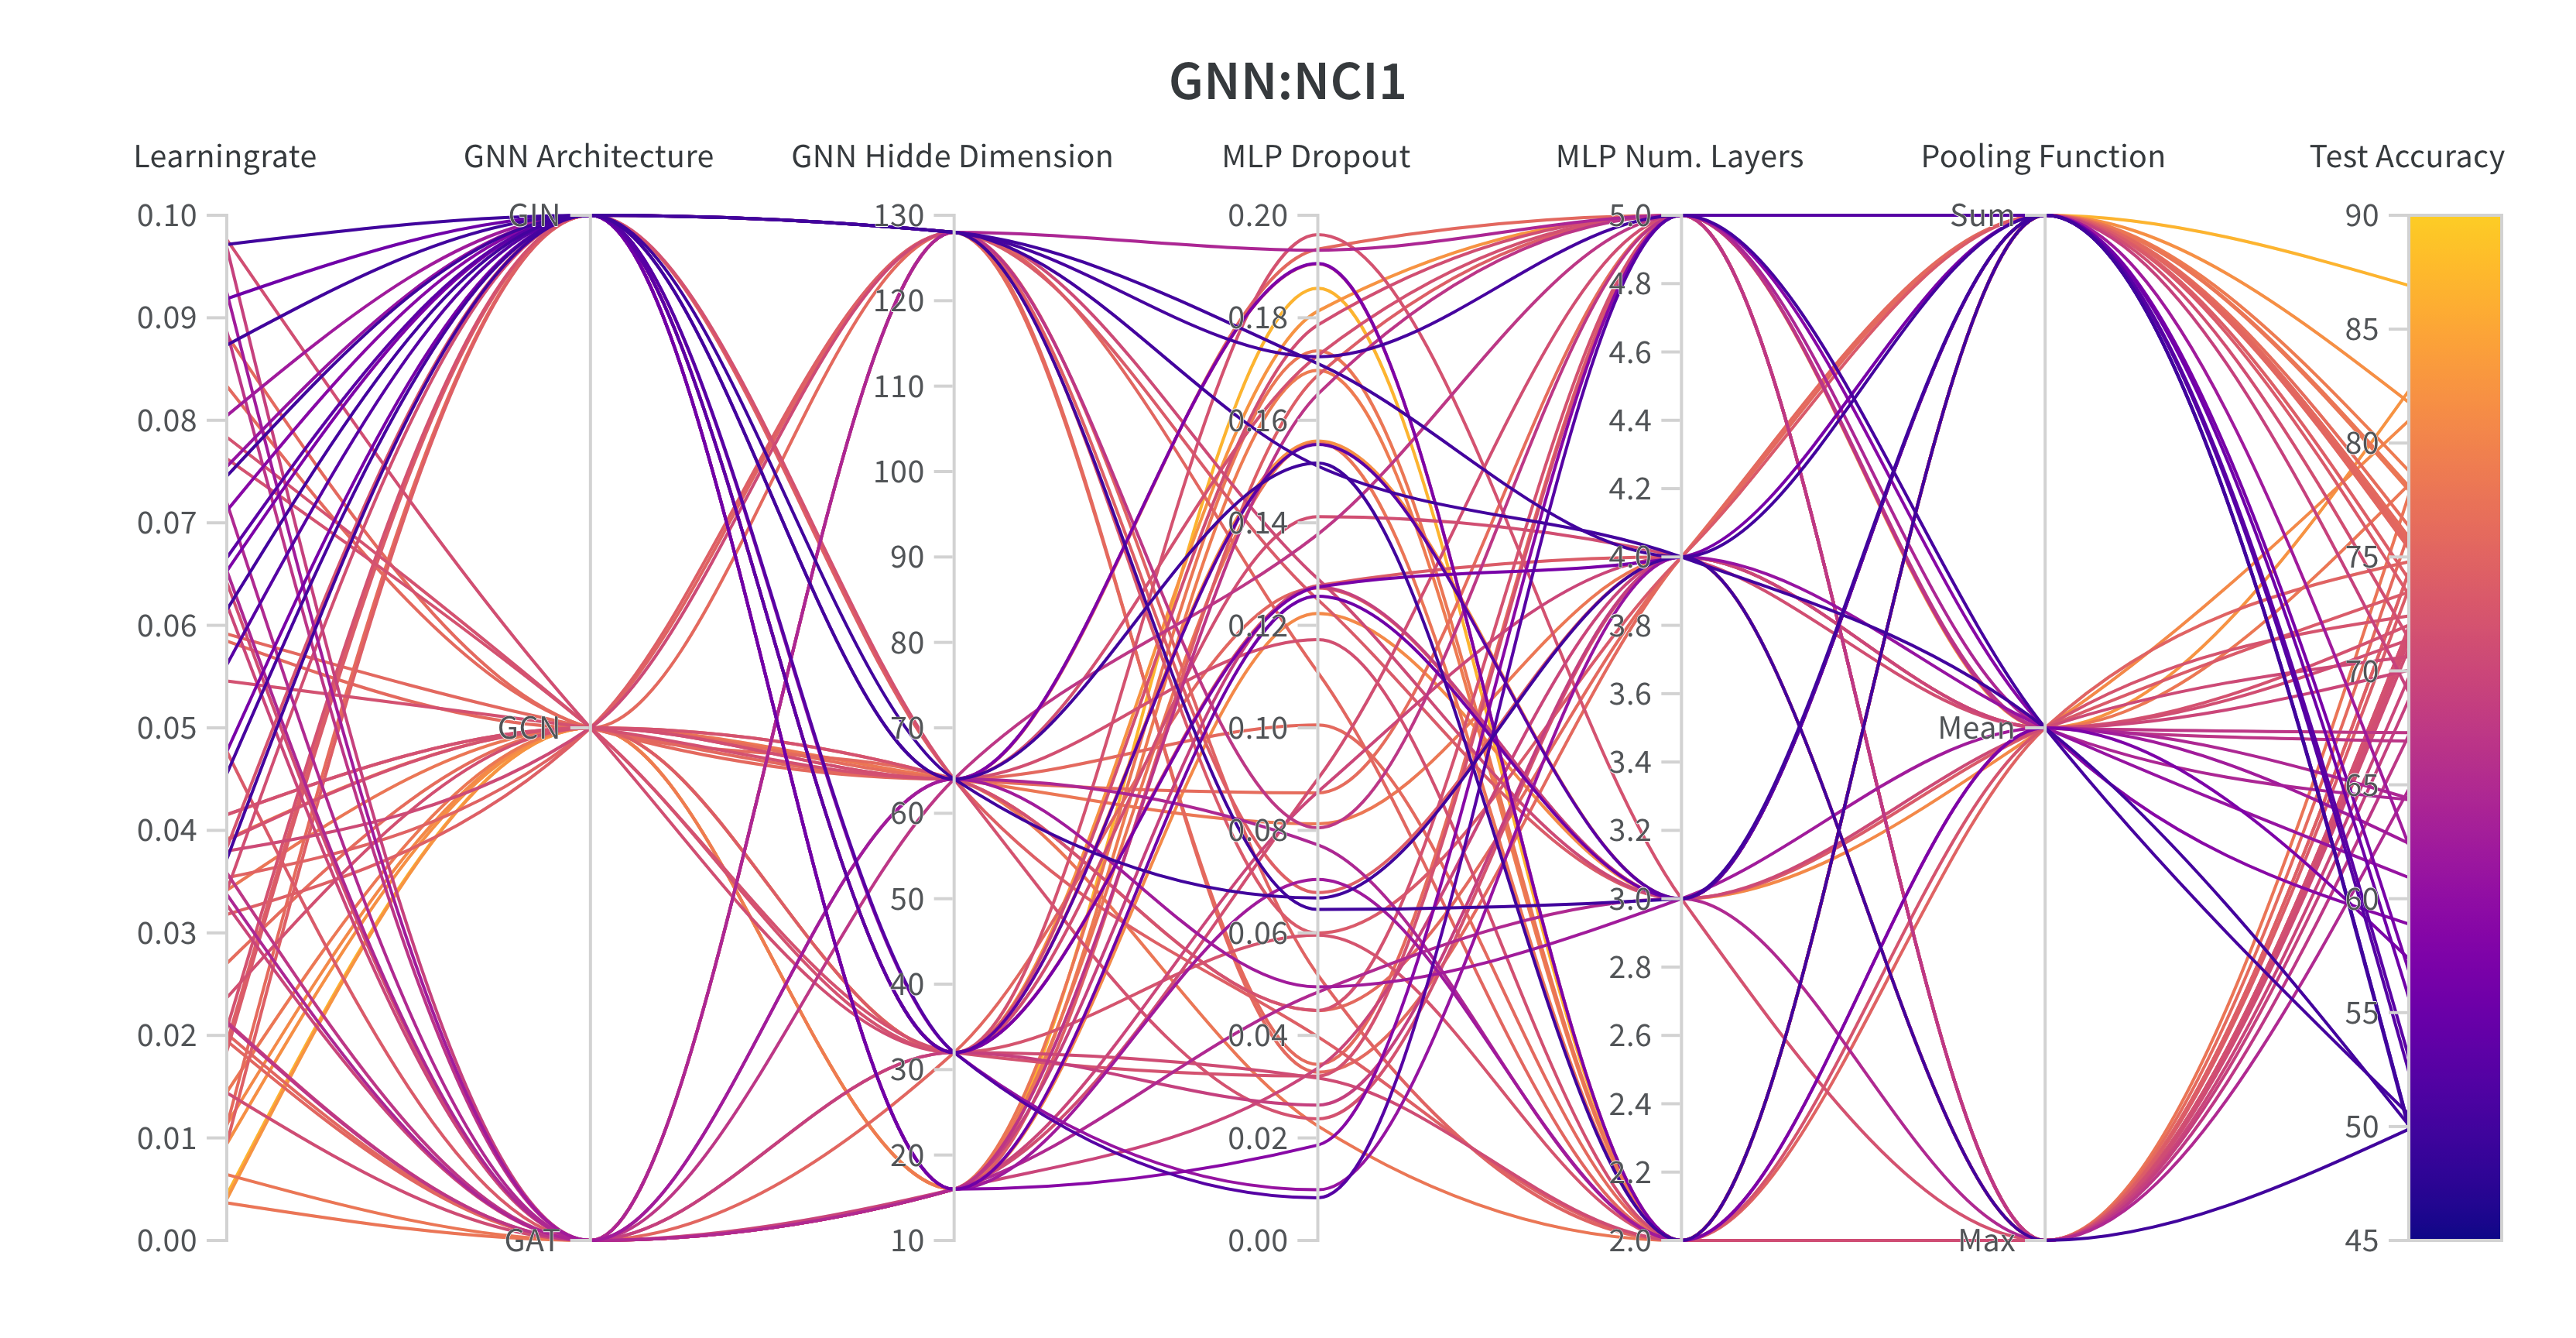
\includegraphics[width=\textwidth, trim={0 75 0 150}, clip]{Figures/hyperparameter_gnn_reddit.png}
    \caption{Overview of the effects of each hyperparameter on the accuracy of the corresponding configured \gnn model for the \reddit dataset.}
    \label{fig:wandb_gnn_reddit}
\end{figure}
\clearpage

\subsection{Overview of the Number of Configurations}
\begin{table}[H]
	\caption{Overview of the number of different configurations tested for each model type and each dataset.}
	\label{tab:num_runs}
    \resizebox{.975\textwidth}{!}{ 	\renewcommand{\arraystretch}{1.05}
		\begin{tabular}{@{}c <{\enspace}@{}lcccccccccc@{}}	\toprule
			& \multirow{3}{*}{\vspace*{4pt}\textbf{Model}}&\multicolumn{10}{c}{\textbf{Dataset}}\\\cmidrule{3-12}
            & & \multicolumn{6}{c}{\textbf{Classification}} & \multicolumn{4}{c}{\textbf{Regression}}\\\cmidrule(lr){3-8}\cmidrule(lr){9-12}
			& & \enzymes & \imdb & \mutag & \nci & \proteins & \reddit & \alchemy & \alchemyten & \zinc & \zincten
			\\
			\toprule
			\multirow[c]{7}{*}{\rotatebox{90}{\wlnn}} 	&
			\textsf{Max} & 86 & 70 & 150 & 26 & 35 & 40 & 0 & 0 & 0 & 0 \\
			& \textsf{Mean} & 76 & 67 & 120 & 19 & 27 & 40 & 0 & 0 & 0 & 0 \\
			& \textsf{Sum} &  85 & 67 & 130 & 14 & 29 & 41 & 0 & 0 & 0 & 0 \\  
			\cmidrule{2-12}  		
			& \textsf{Embedding-Max} & 338 & 282 & 290 & 79 & 245 & 45 & 3 & 95 & 6 & 33 \\
			& \textsf{Embedding-Mean} & 288 & 271 & 299 & 109 & 216 & 50 & 6 & 77 & 8 & 24 \\ 
			& \textsf{Embedding-Sum} & 296 & 293 & 302 & 79 & 215 & 48 & 5 & 273 & 7 & 18 \\ 
			\cmidrule{1-12}
			\multirow[c]{10}{*}{\rotatebox{90}{Graph Neural Networks}} 
			& \textsf{GAT:Max} & 17 & 17 & 36 & 11 & 10 & 6 & 0 & 0 & 0 & 0 \\
			& \textsf{GAT:Mean} & 28 & 15 & 29 & 12 & 10 & 6 & 0 & 0 & 0 & 0 \\
			& \textsf{GAT:Sum} & 26 & 17 & 37 & 15 & 16 & 6 & 0 & 0 & 0 & 0 \\
			\cmidrule{2-12}
			& \textsf{GCN:Max} & 31 & 22 & 37 & 17 & 10 & 9 & 0 & 0 & 0 & 0 \\
			& \textsf{GCN:Mean} & 19 & 26 & 26 & 19 & 16 & 5 & 0 & 0 & 0 & 0 \\
			& \textsf{GCN:Sum} & 30 & 29 & 27 & 17 & 14 & 10 & 0 & 0 & 0 & 0 \\  
			\cmidrule{2-12}	
			& \textsf{GIN:Max} & 21 & 17 & 28 & 25 & 20 & 3 & 1 & 1 & 1 & 1 \\
			& \textsf{GIN:Mean} & 31 & 9 & 31 & 18 & 26 & 9 & 2 & 2 & 2 & 2 \\
			& \textsf{GIN:Sum} & 26 & 9 & 36 & 20 & 11 & 9 & 1 & 1 & 1 & 1 \\
            \cmidrule{1-12}
            \multirow[c]{10}{*}{\rotatebox{90}{\wl:\gnn}} 
			& \textsf{GAT:Max} & 2 & 4 & 1 & 9 & 4 & 2 & 0 & 0 & 0 & 0 \\
			& \textsf{GAT:Mean} & 3 & 4 & 6 & 6 & 7 & 4 & 0 & 0 & 0 & 0 \\
			& \textsf{GAT:Sum} & 5 & 5 & 6 & 9 & 4 & 4 & 0 & 0 & 0 & 0 \\
			\cmidrule{2-12}
			& \textsf{GCN:Max} & 2 & 6 & 4 & 12 & 6 & 3 & 0 & 0 & 0 & 0 \\
			& \textsf{GCN:Mean} & 3 & 5 & 3 & 10 & 8 & 2 & 0 & 0 & 0 & 0 \\
			& \textsf{GCN:Sum} & 6 & 2 & 3 & 5 & 5 & 3 & 0 & 0 & 0 & 0 \\
			\cmidrule{2-12}	
			& \textsf{GIN:Max} & 3 & 4 & 4 & 9 & 7 & 5 & 0 & 0 & 0 & 0 \\
			& \textsf{GIN:Mean} & 2 & 6 & 2 & 10 & 7 & 3 & 0 & 0 & 0 & 0 \\
			& \textsf{GIN:Sum} & 4 & 2 & 4 & 11 & 4 & 4 & 0 & 0 & 0 & 0 \\
			\bottomrule
		\end{tabular}}            
\end{table}


\section{GNN Approximation Evaluation}

\subsection{Unique Color Count utilized by \wl Algorithm}

\begin{table}[H]
    \caption{Overview of the number of unique colors in the colorings computed by the \wl algorithm when applied to each dataset. Specifically, we specified the number of iterations of the \wl algorithm. Additionally, the ``\# Nodes'' column showcases the maximum number of unique colors that can appear in the colorings.}
    \label{tab:unique_colors}
    \centering
    \resizebox{\textwidth}{!}{ 	\renewcommand{\arraystretch}{0.9}
    \begin{tabular}{@{}c <{\enspace}@{}lrrrrrrrrrrr | r@{}}
    \toprule
        & \multirow{3}{*}{\vspace*{4pt}\textbf{Dataset}}&\multicolumn{11}{c}{\textbf{Number of \wl Iterations}}\\\cmidrule{3-14}
        & & 0 & 1 & 2 & 3 & 4 & 5 & 6 & 7 & 8 & 9 & 10 & \# Nodes\\
        \midrule
        \multirow{6}{*}{\rotatebox{90}{Classification}}
        & \enzymes & 2 & 231 & 10\,416 & 15\,208 & 16\,029 & 16\,450 & 16\,722 & 16\,895 & 17\,026 & 17\,130 & 17\,204 & 195\,80\\
        & \imdb & 1 & 65 & 2\,931 & 3\,595 & 3\,595 & 3\,595 & 3\,595 & 3\,595 & 3\,595 & 3\,595 & 3\,595 & 19\,773 \\
        & \mutag & 2 & 33 & 174 & 572 & 1\,197 & 1\,766 & 2\,167 & 2\,403 & 2\,511 & 2\,560 & 2\,579 & 3\,371 \\
        & \nci & 2 & 292 & 4\,058 & 22\,948 & 44\,508 & 58\,948 & 68\,632 & 75\,754 & 81\,263 & 85\,590 & 88\,968 & 122\,747\\
        & \proteins & 2 & 297 & 20\,962 & 35\,676 & 37\,940 & 38\,653 & 38\,926 & 39\,064 & 39\,141 & 39\,180 & 39\,203 & 43\,471\\
        & \reddit & 1 & 566 & 71\,893 & 244\,529 & 317\,728 & 333\,258 & 335\,961 & 336\,412 & 336\,490 & 336\,506 & 336\,507 & 859\,254 \\
        \cmidrule{2-14}
        \multirow{4}{*}{\rotatebox{90}{Regress.}}
        & \alchemy & 2 & 70 & 4\,782 & 164\,224 & 620\,332 & 995\,264 & 1\,166\,951 & 1\,216\,094 & 1\,225\,861 & 1\,227\,632 & 1\,227\,904 & 2\,046\,329\\
        & \alchemyten & 2 & 70 & 2\,764 & 33\,903 & 76\,822 & 98\,394 & 104\,687 & 105\,907 & 106\,109 & 106\,149 & 106\,166 & 121\,422\\
        & \zinc & 2 & 773 & 288\,74 & 290\,473 & 1\,000\,917 & 1\,977\,437 & 2\,921\,087 & 3\,690\,341 & 4\,270\,959 & 4\,681\,881 & 4\,945\,363 & 5\,775\,257 \\
        & \zincten & 2 & 392 & 9\,818 & 61\,198 & 132\,862 & 185\,699 & 216\,210 & 233\,484 & 242\,866 & 247\,688 & 249\,971 & 278\,179 \\
        \bottomrule
    \end{tabular}}
\end{table}
\clearpage

\subsubsection{\gnn Approximation Performance on the ENZYMES Dataset}

\begin{figure}[H]
    \centering
    \begin{minipage}[b]{0.45992852703\textwidth}
        \centering
        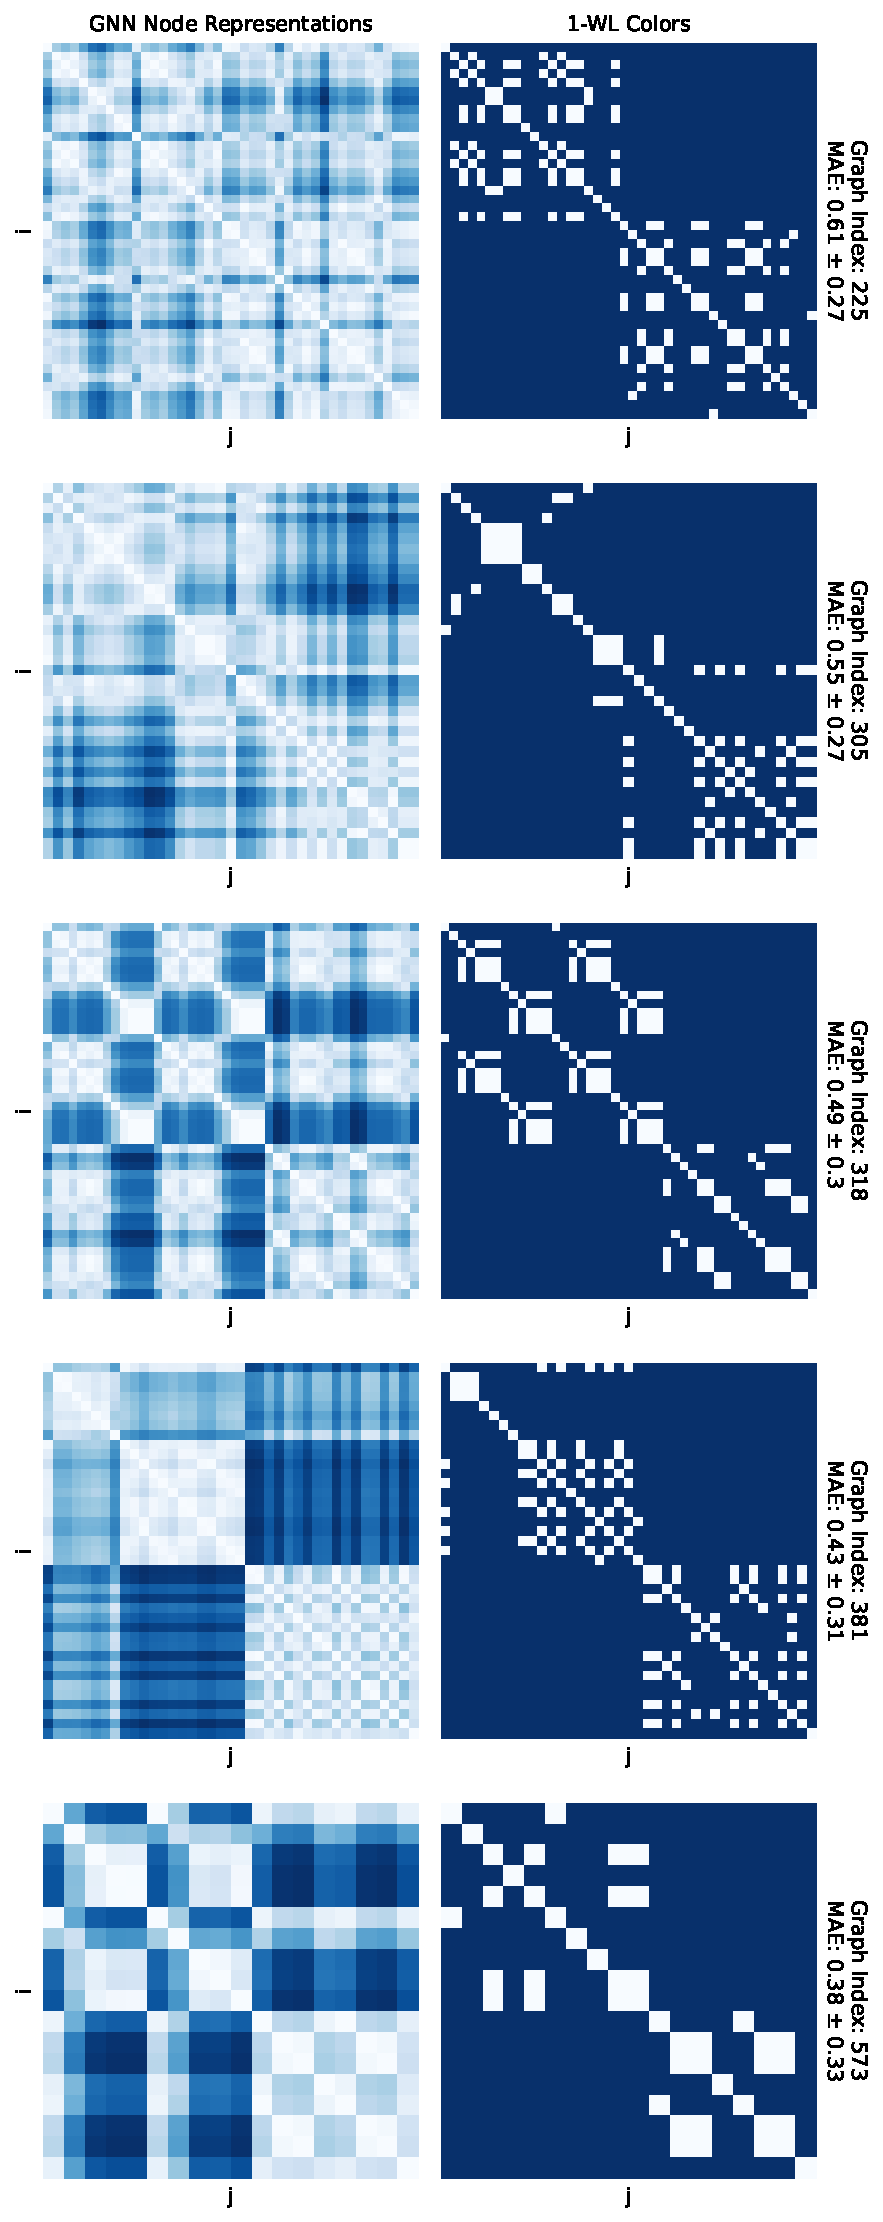
\includegraphics[width=\textwidth, left]{Figures/heatmaps_ENZYMES_0.pdf}
    \end{minipage}
    \hfill
    \begin{minipage}[b]{0.53007147296\textwidth}
        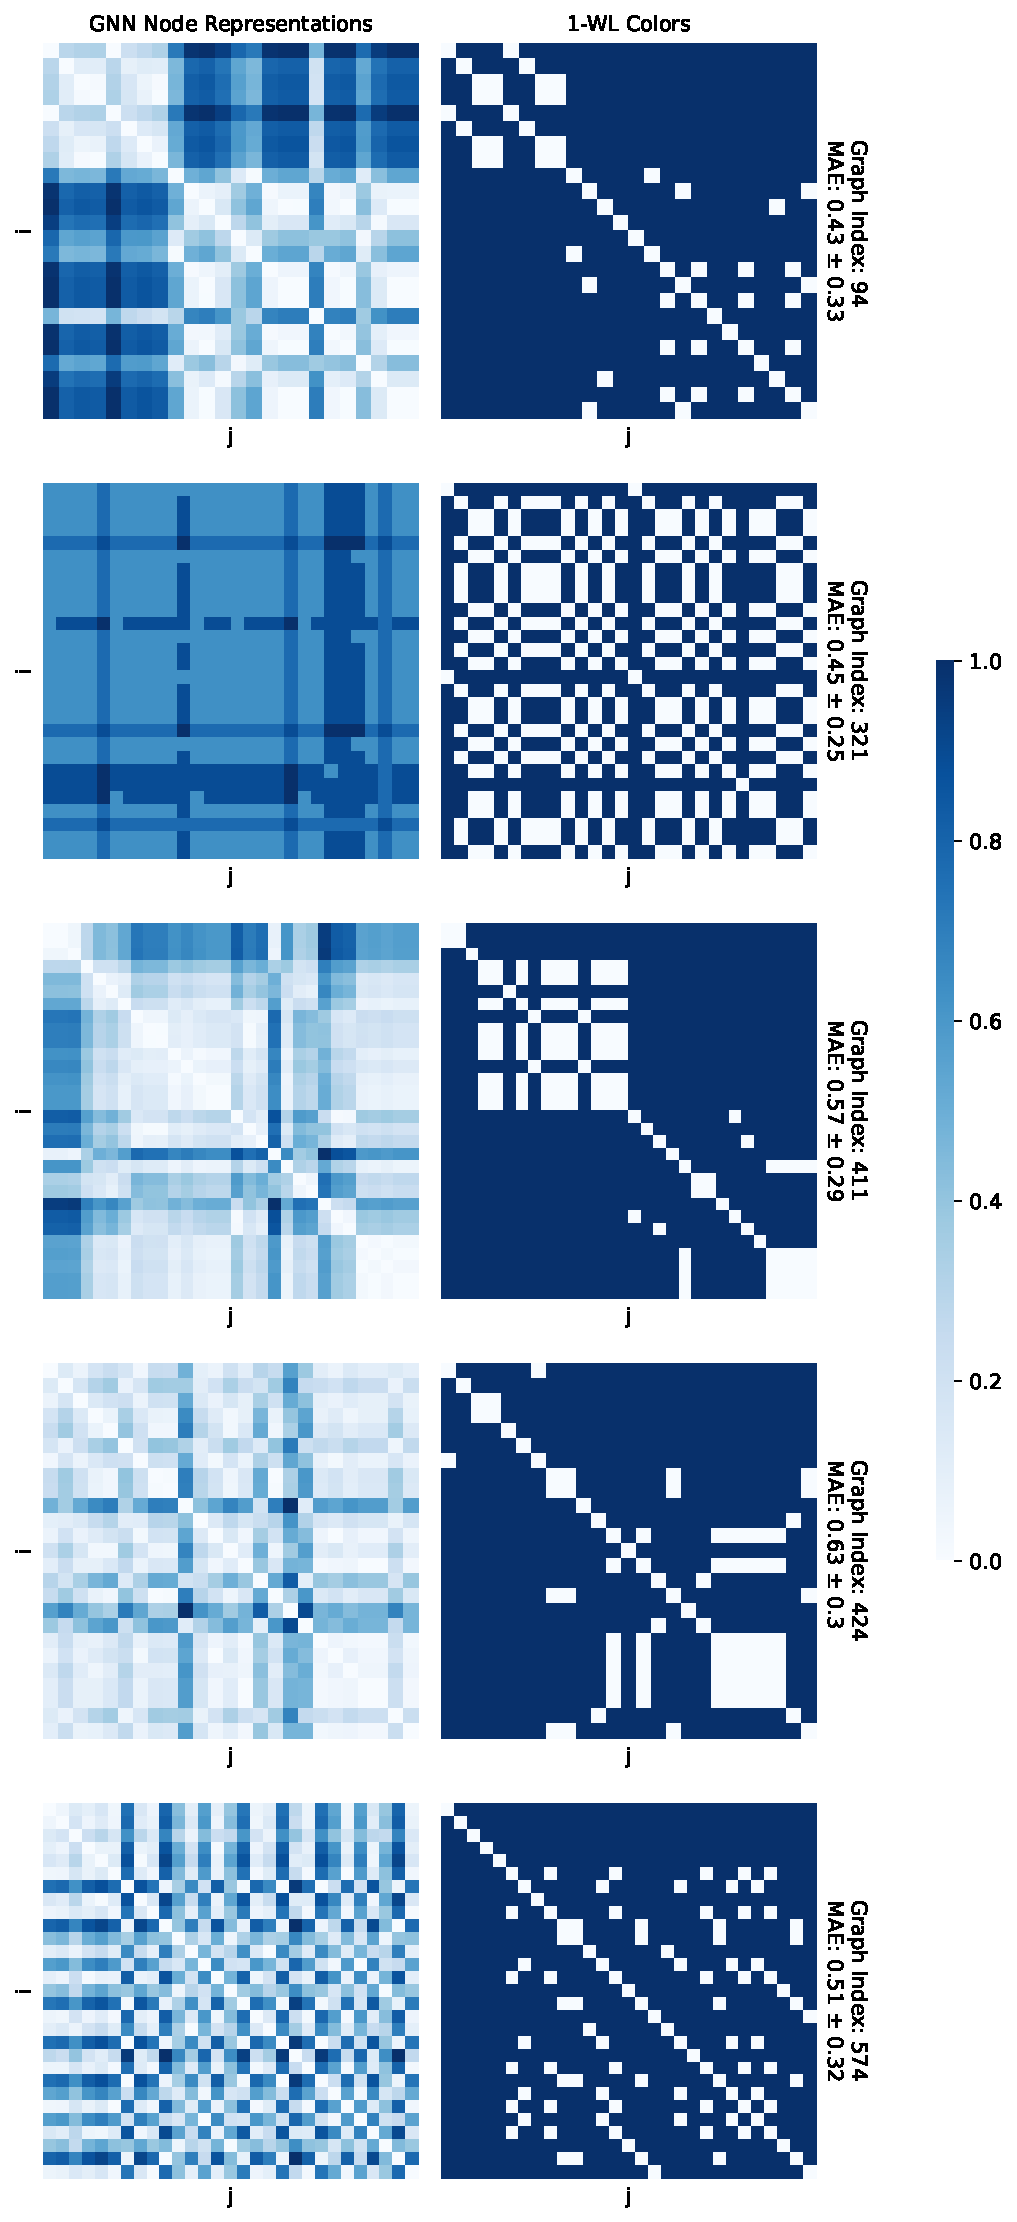
\includegraphics[width=\textwidth, right]{Figures/heatmaps_ENZYMES_1.pdf}
    \end{minipage}
    \hfill
    \caption{Visualizing the performance of the best performing \gnn on the \textsc{Enzymes} dataset in approximating node colors computed by the \wl algorithm. The ten graphs shown are randomly sampled from the \gnn's test set. The average error for the entire test set is $0.49 \pm 0.3$.}
    \label{fig:gnn_approx_enzymes}
\end{figure}
\clearpage

\subsubsection{\gnn Approximation Performance on the IMDB-BINARY Dataset}
\begin{figure}[H]
    \centering
    \begin{minipage}[b]{0.45992852703\textwidth}
        \centering
        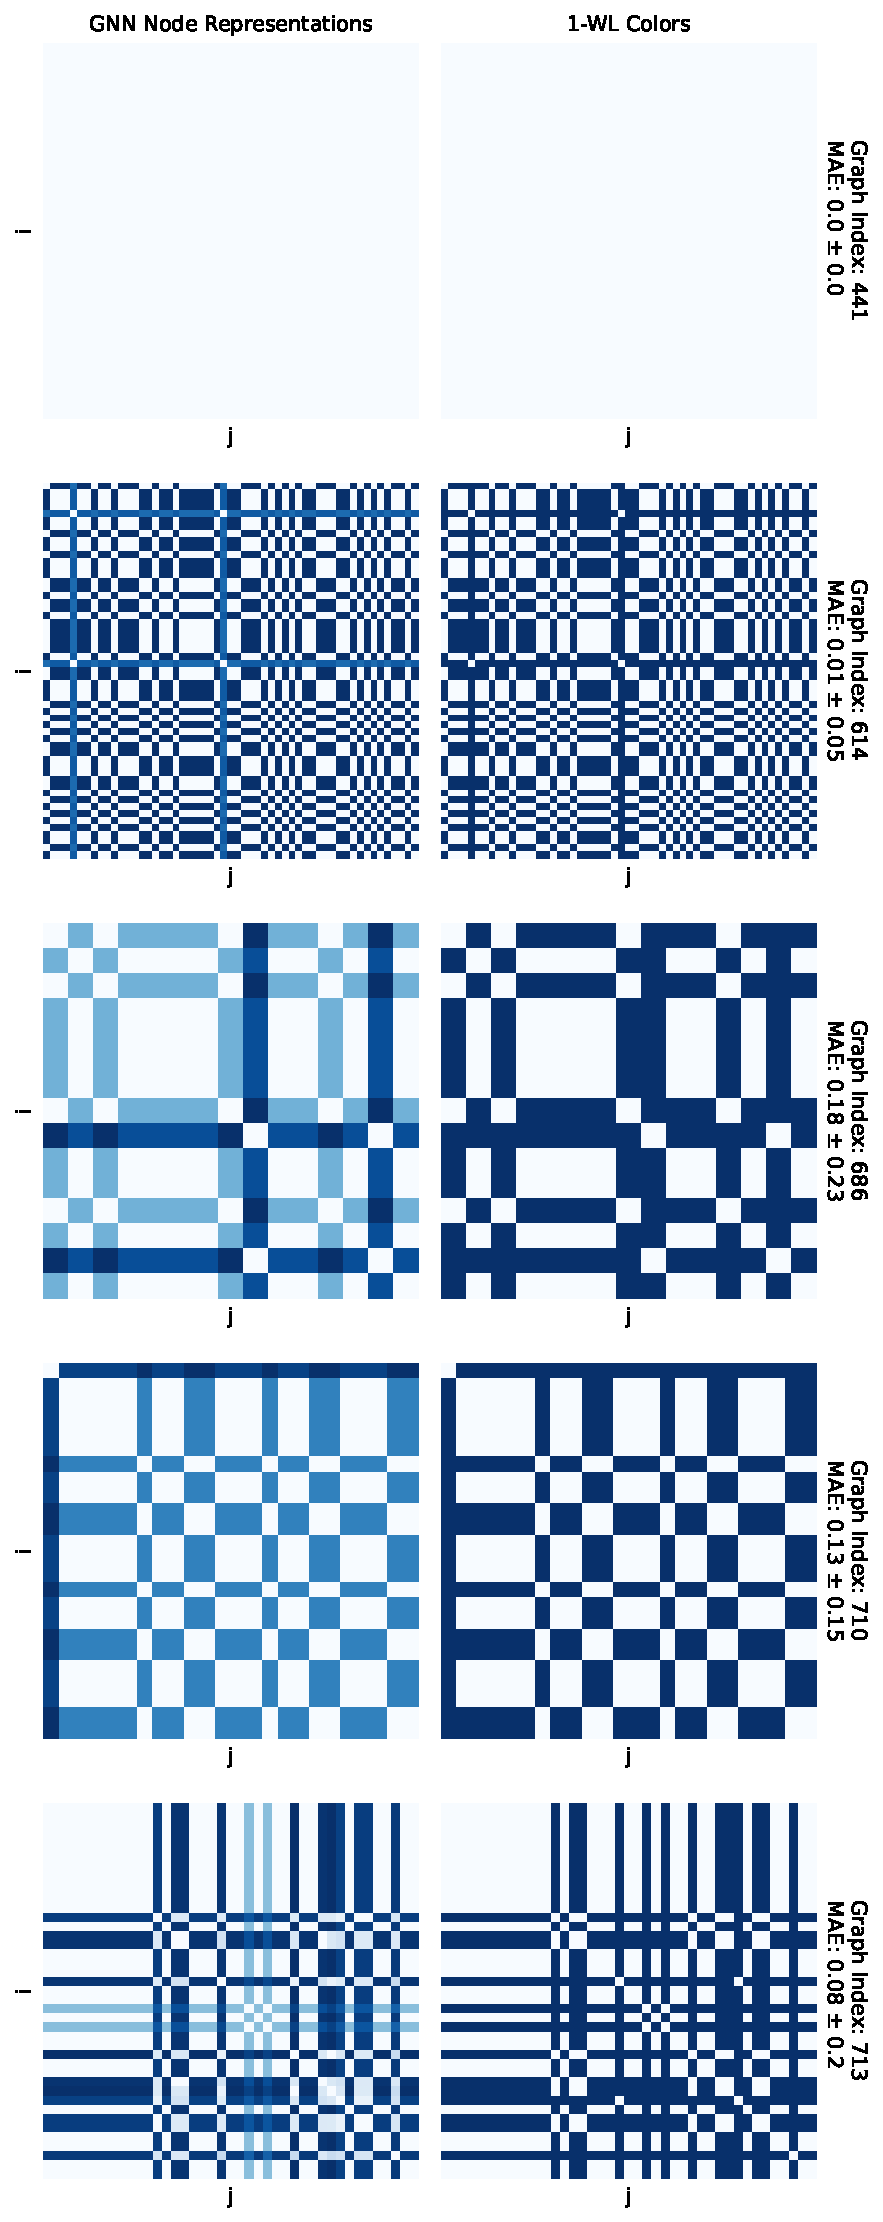
\includegraphics[width=\textwidth, left]{Figures/heatmaps_IMDB-BINARY_0.pdf}
    \end{minipage}
    \hfill
    \begin{minipage}[b]{0.53007147296\textwidth}
        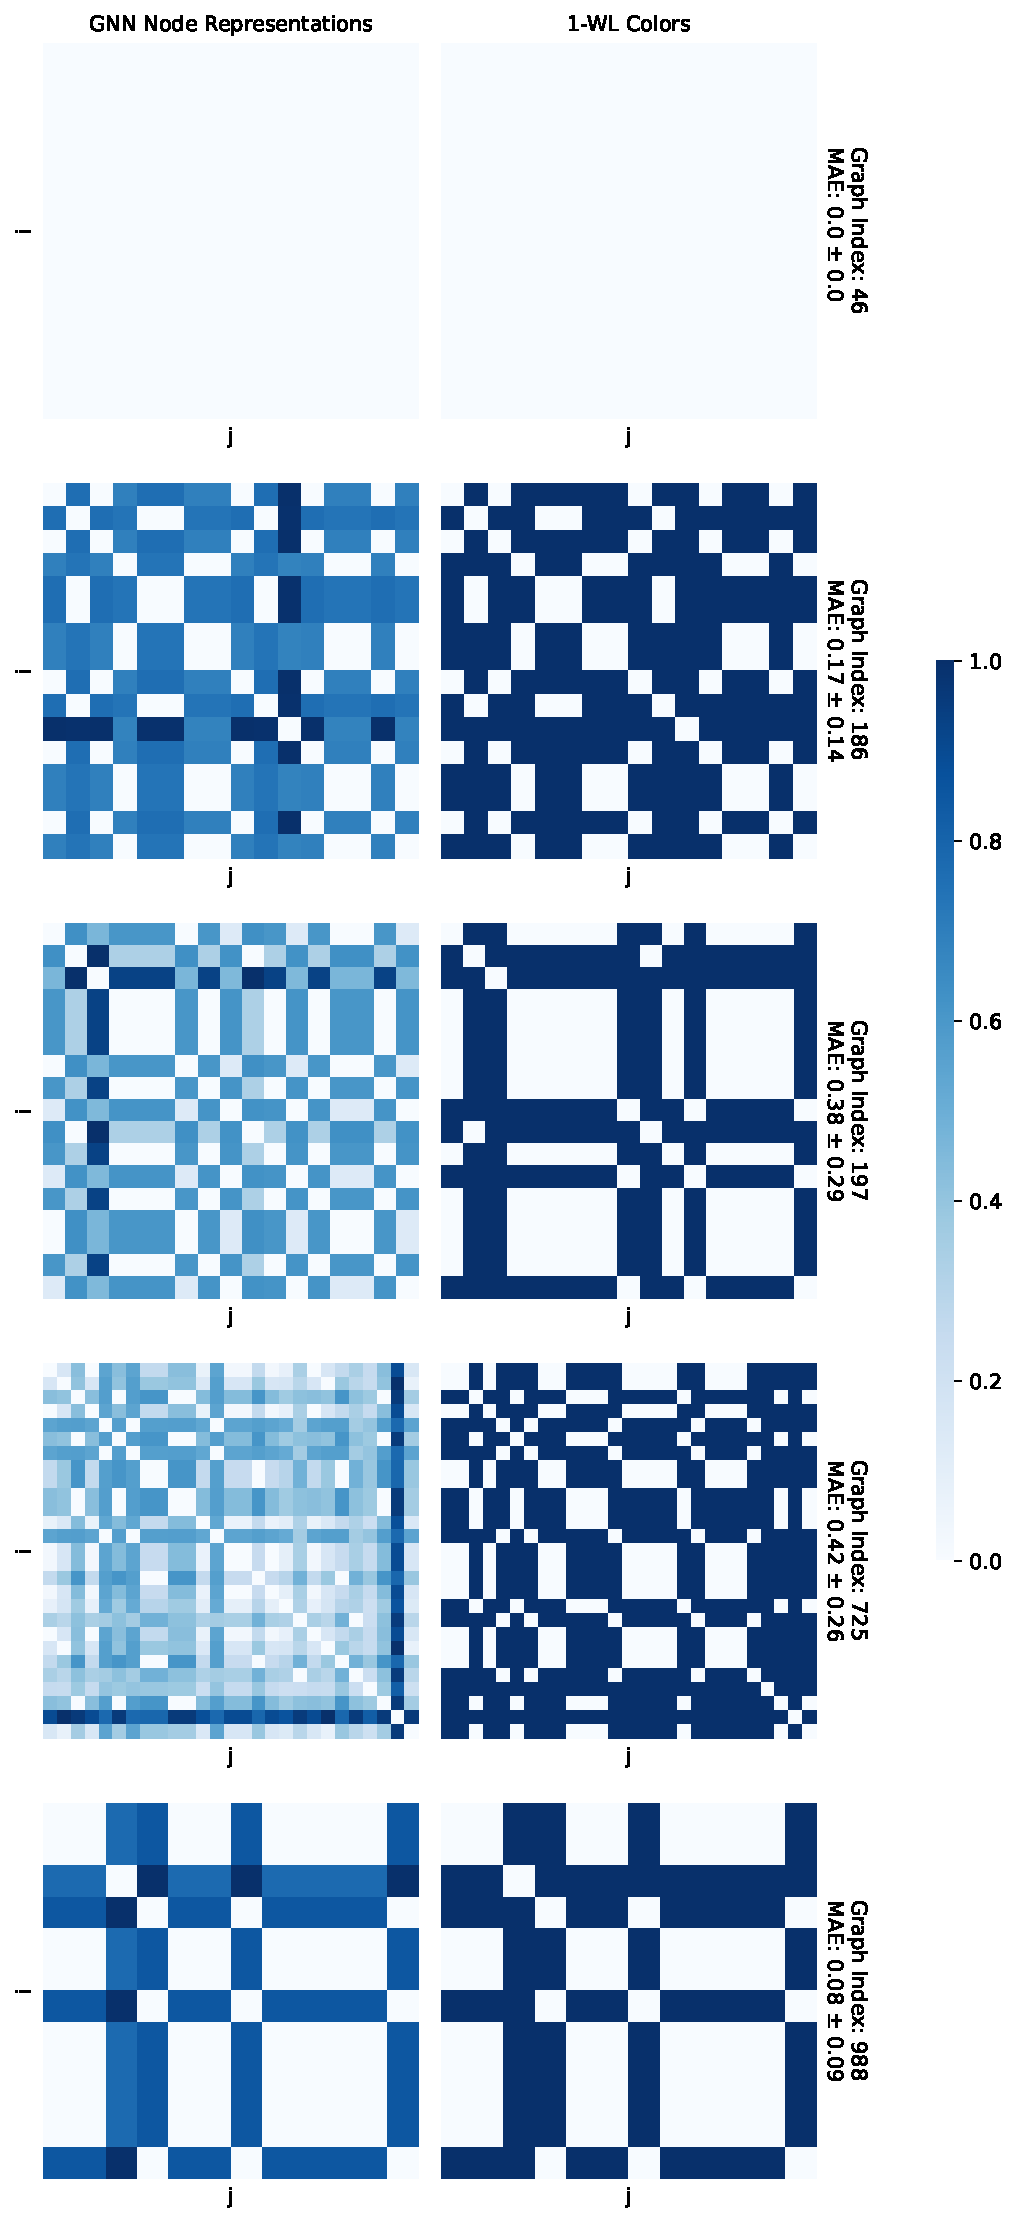
\includegraphics[width=\textwidth, right]{Figures/heatmaps_IMDB-BINARY_1.pdf}
    \end{minipage}
    \hfill
    \caption{Visualizing the performance of the best performing \gnn on the \textsc{Imdb-Binary} dataset in approximating node colors computed by the \wl algorithm. The ten graphs shown are randomly sampled from the \gnn's test set. The average error for the entire test set is $0.14 \pm 0.15$.}
    \label{fig:gnn_approx_imdb}
\end{figure}
\clearpage

\subsubsection{\gnn Approximation Performance on the MUTAG Dataset}
\begin{figure}[H]
    \centering
    \begin{subfigure}[b]{0.45992852703\textwidth}
        \centering
        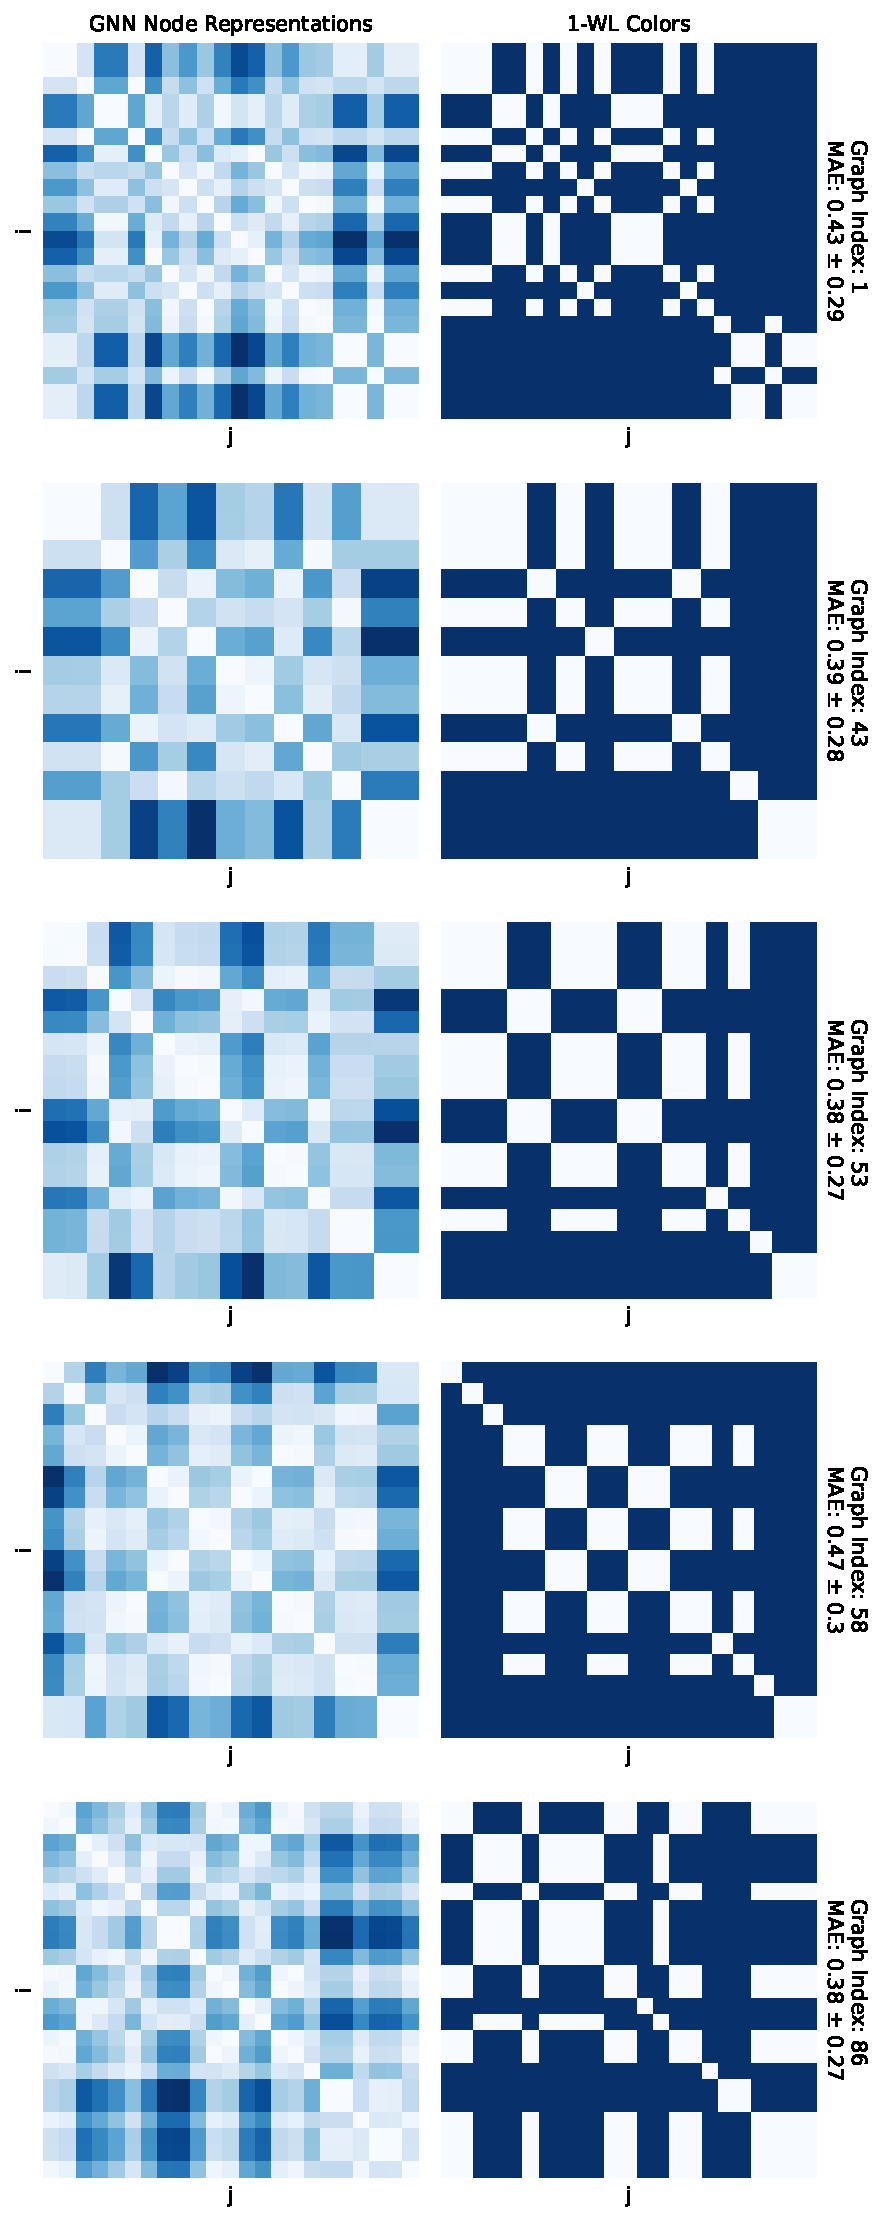
\includegraphics[width=\textwidth, left]{Figures/heatmaps_MUTAG_0.pdf}
    \end{subfigure}
    \hfill
    \begin{subfigure}[b]{0.53007147296\textwidth}
        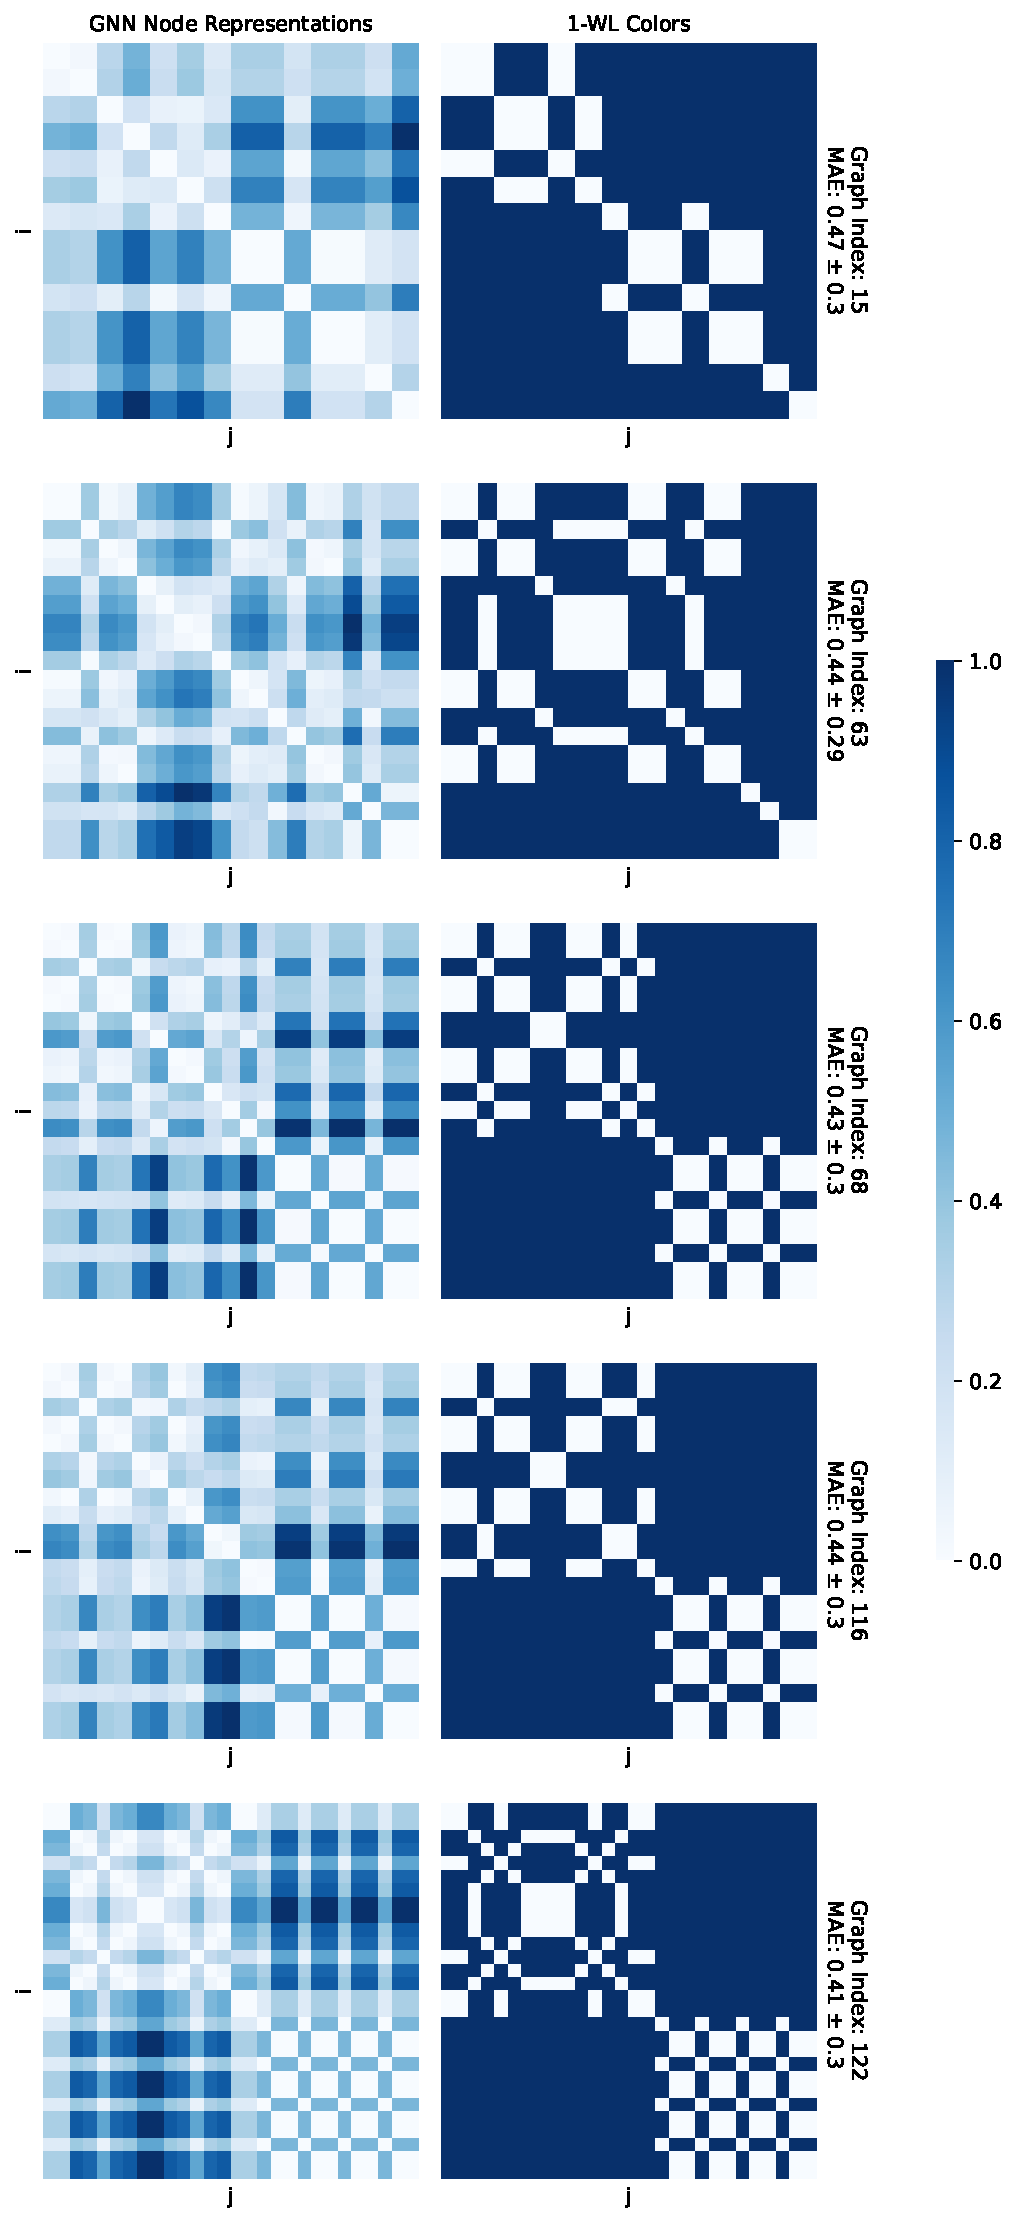
\includegraphics[width=\textwidth, right]{Figures/heatmaps_MUTAG_1.pdf}
    \end{subfigure}
    \hfill
    \caption{Visualizing the performance of the best performing \gnn on the \textsc{Mutag} dataset in approximating node colors computed by the \wl algorithm. The ten graphs shown are randomly sampled from the \gnn's test set. The average error for the entire test set is $0.42 \pm 0.29$.}
    \label{fig:gnn_approx_mutag}
\end{figure}
\clearpage

\subsubsection{\gnn Approximation Performance on the NCI1 Dataset}
\begin{figure}[H]
    \centering
    \begin{minipage}[b]{0.45992852703\textwidth}
        \centering
        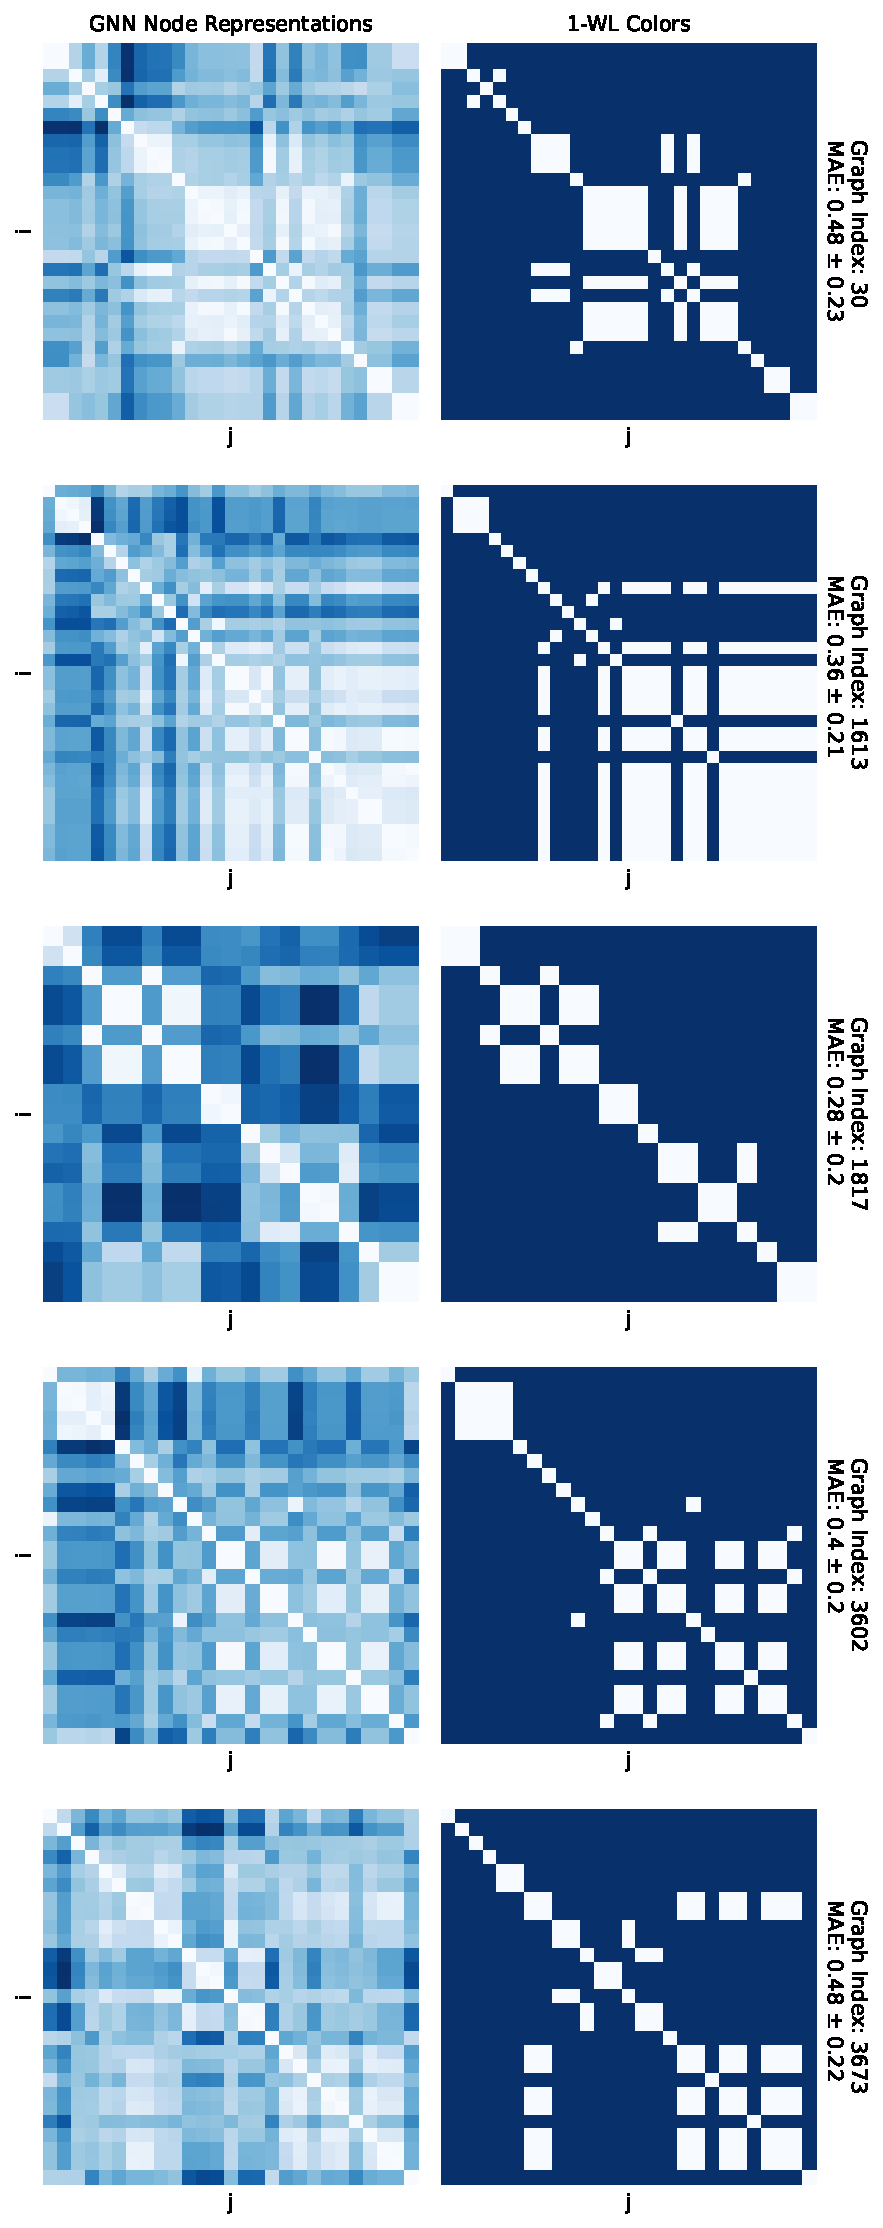
\includegraphics[width=\textwidth, left]{Figures/heatmaps_NCI1_0_k_wl_1.pdf}
    \end{minipage}
    \hfill
    \begin{minipage}[b]{0.53007147296\textwidth}
        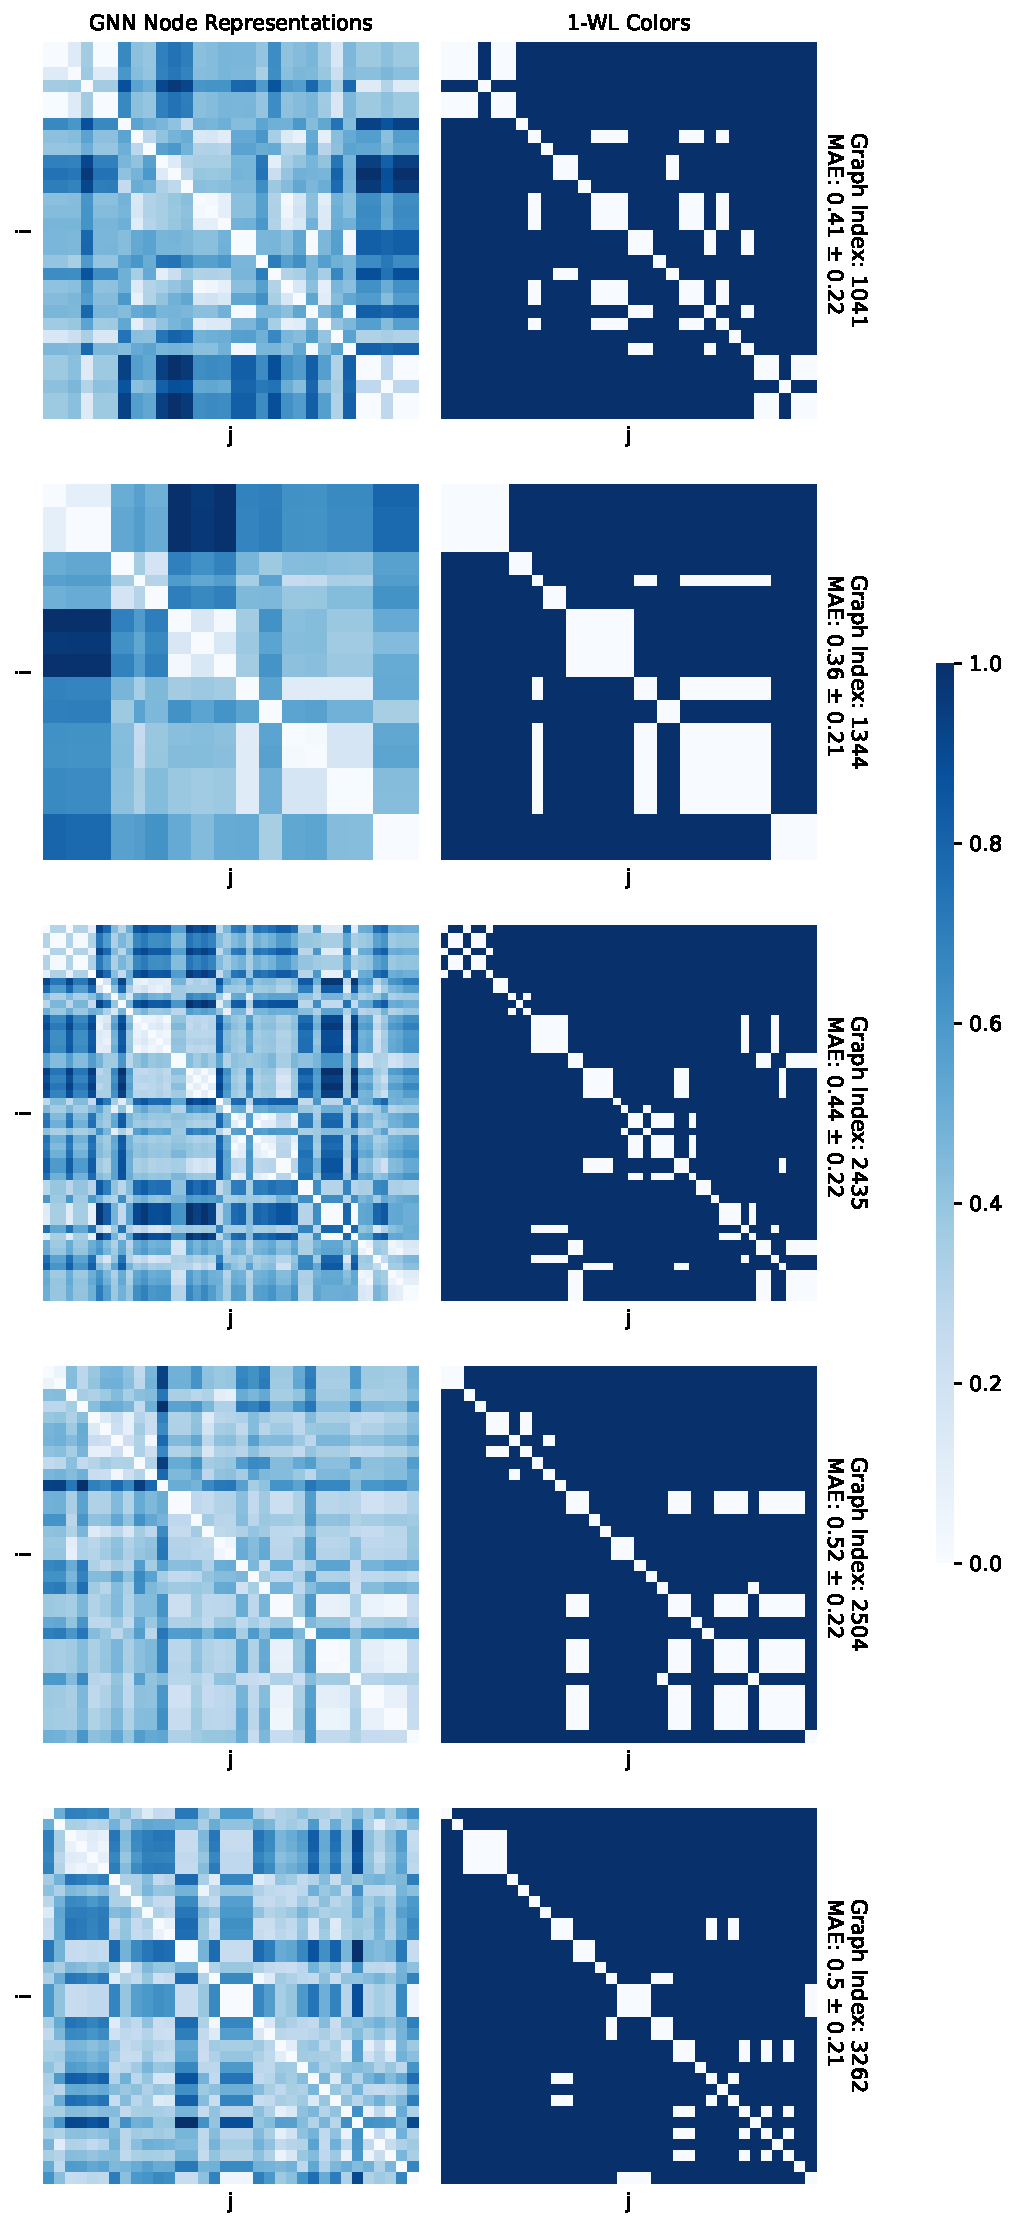
\includegraphics[width=\textwidth, right]{Figures/heatmaps_NCI1_1_k_wl_1.pdf}
    \end{minipage}
    \hfill
    \caption{Visualizing the performance of the best performing \gnn on the \textsc{Nci1} dataset in approximating node colors computed by the \wl algorithm. The ten graphs shown are randomly sampled from the \gnn's test set. The average error for the entire test set is $0.42 \pm 0.22$.}
    \label{fig:gnn_approx_nci_1}
\end{figure}
\clearpage

\subsubsection{\gnn Approximation Performance for three \wl Iterations on the NCI1 Dataset}
\begin{figure}[H]
    \centering
    \begin{minipage}[b]{0.45992852703\textwidth}
        \centering
        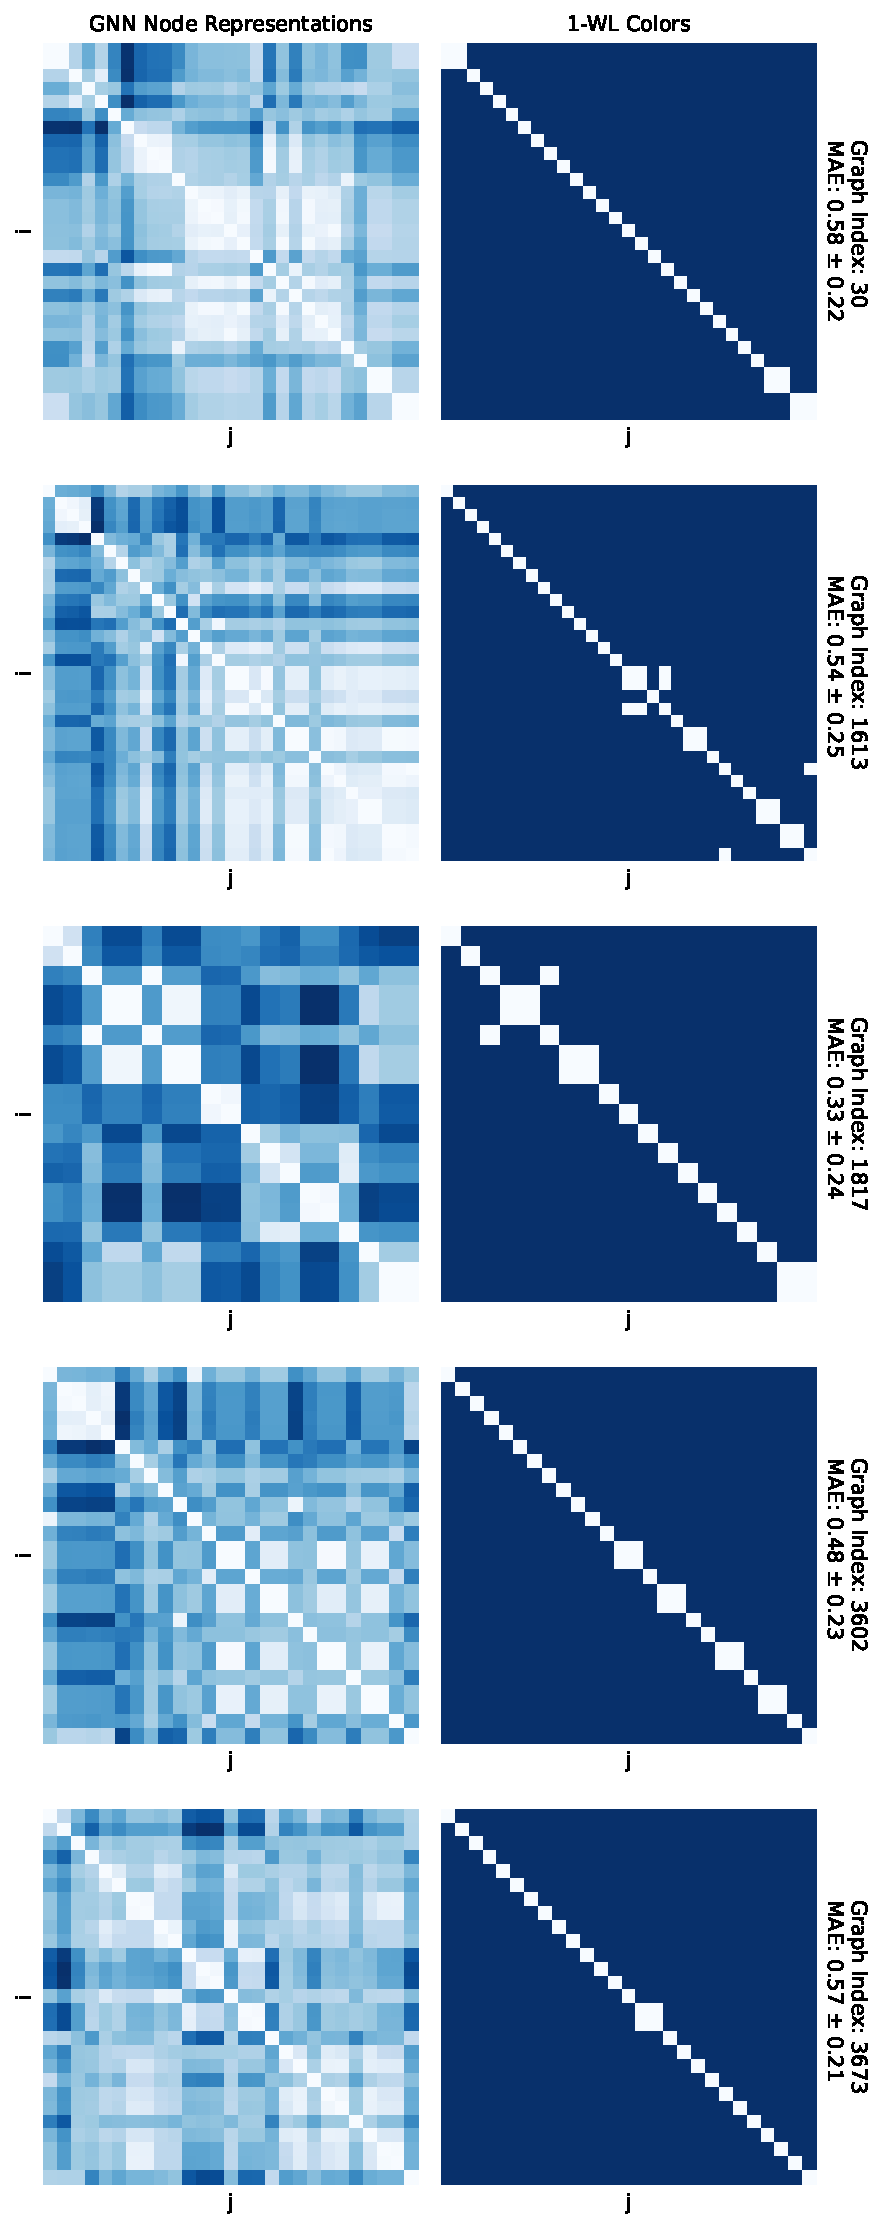
\includegraphics[width=\textwidth, left]{Figures/heatmaps_NCI1_0.pdf}
    \end{minipage}
    \hfill
    \begin{minipage}[b]{0.53007147296\textwidth}
        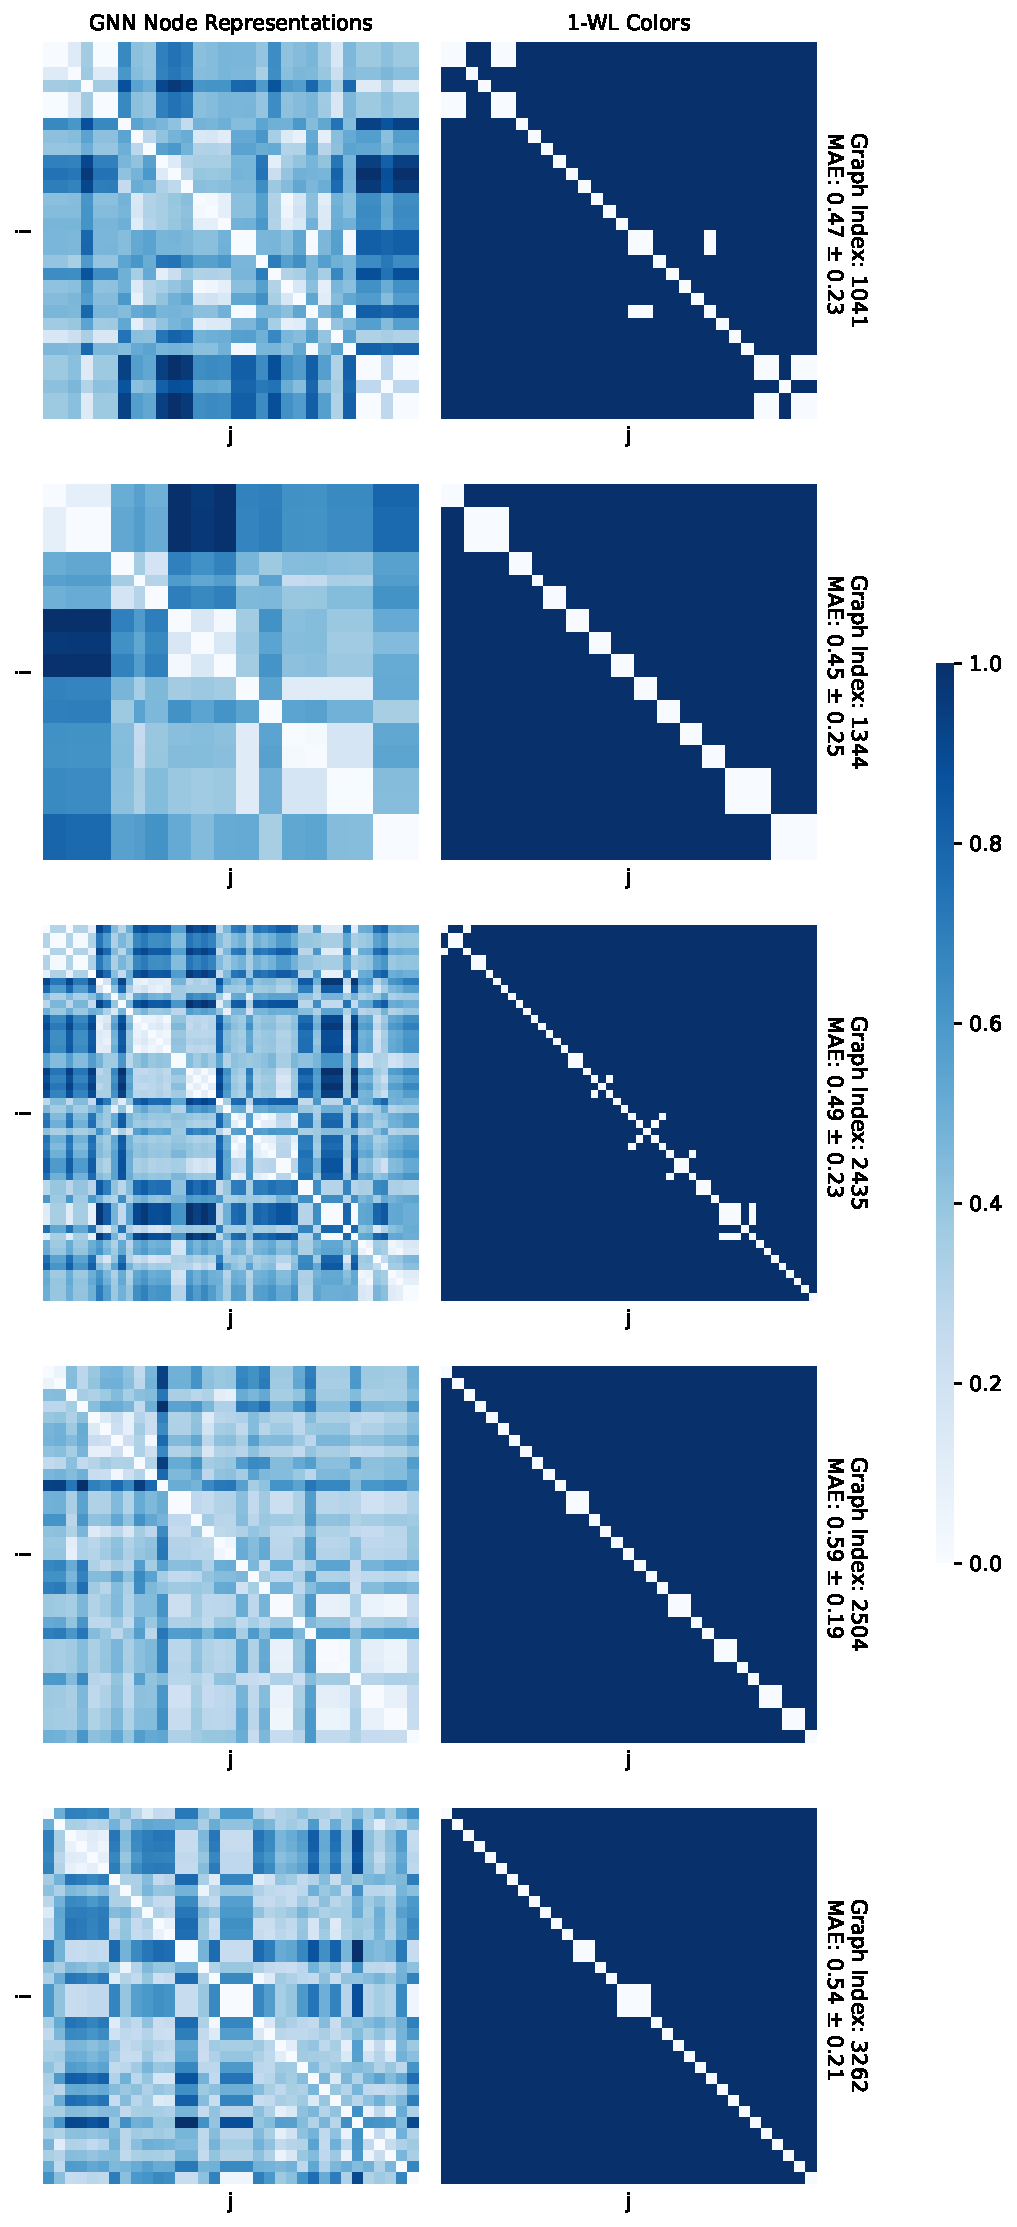
\includegraphics[width=\textwidth, right]{Figures/heatmaps_NCI1_1.pdf}
    \end{minipage}
    \hfill
    \caption{Visualizing the performance of the best performing \gnn on the \textsc{Nci1} dataset in approximating node colors computed by the \wl algorithm. The ten graphs shown are randomly sampled from the \gnn's test set. The average error for the entire test set is $0.50 \pm 0.24$.}
    \label{fig:gnn_approx_nci_3}
\end{figure}
\clearpage


\subsubsection{\gnn Approximation Performance on the PROTEINS Dataset}
\begin{figure}[H]
    \centering
    \begin{minipage}[b]{0.45992852703\textwidth}
        \centering
        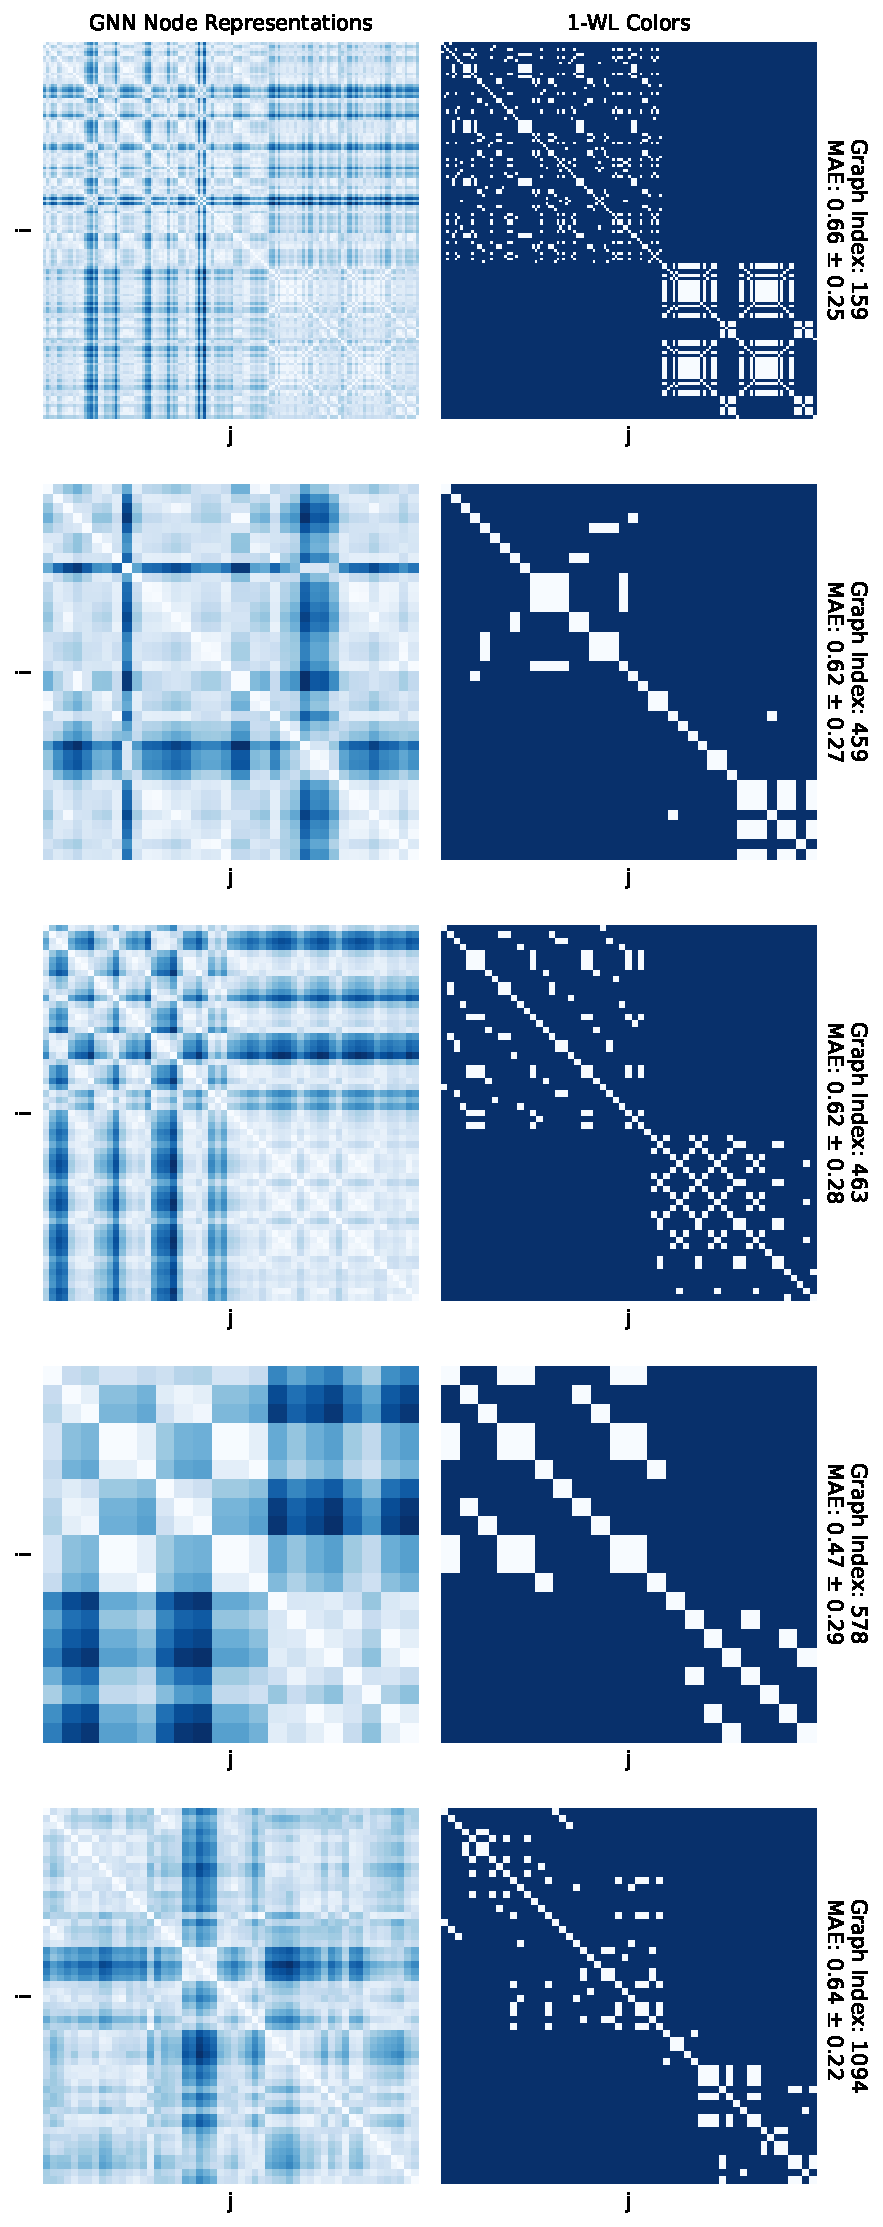
\includegraphics[width=\textwidth, left]{Figures/heatmaps_PROTEINS_0.pdf}
    \end{minipage}
    \hfill
    \begin{minipage}[b]{0.53007147296\textwidth}
        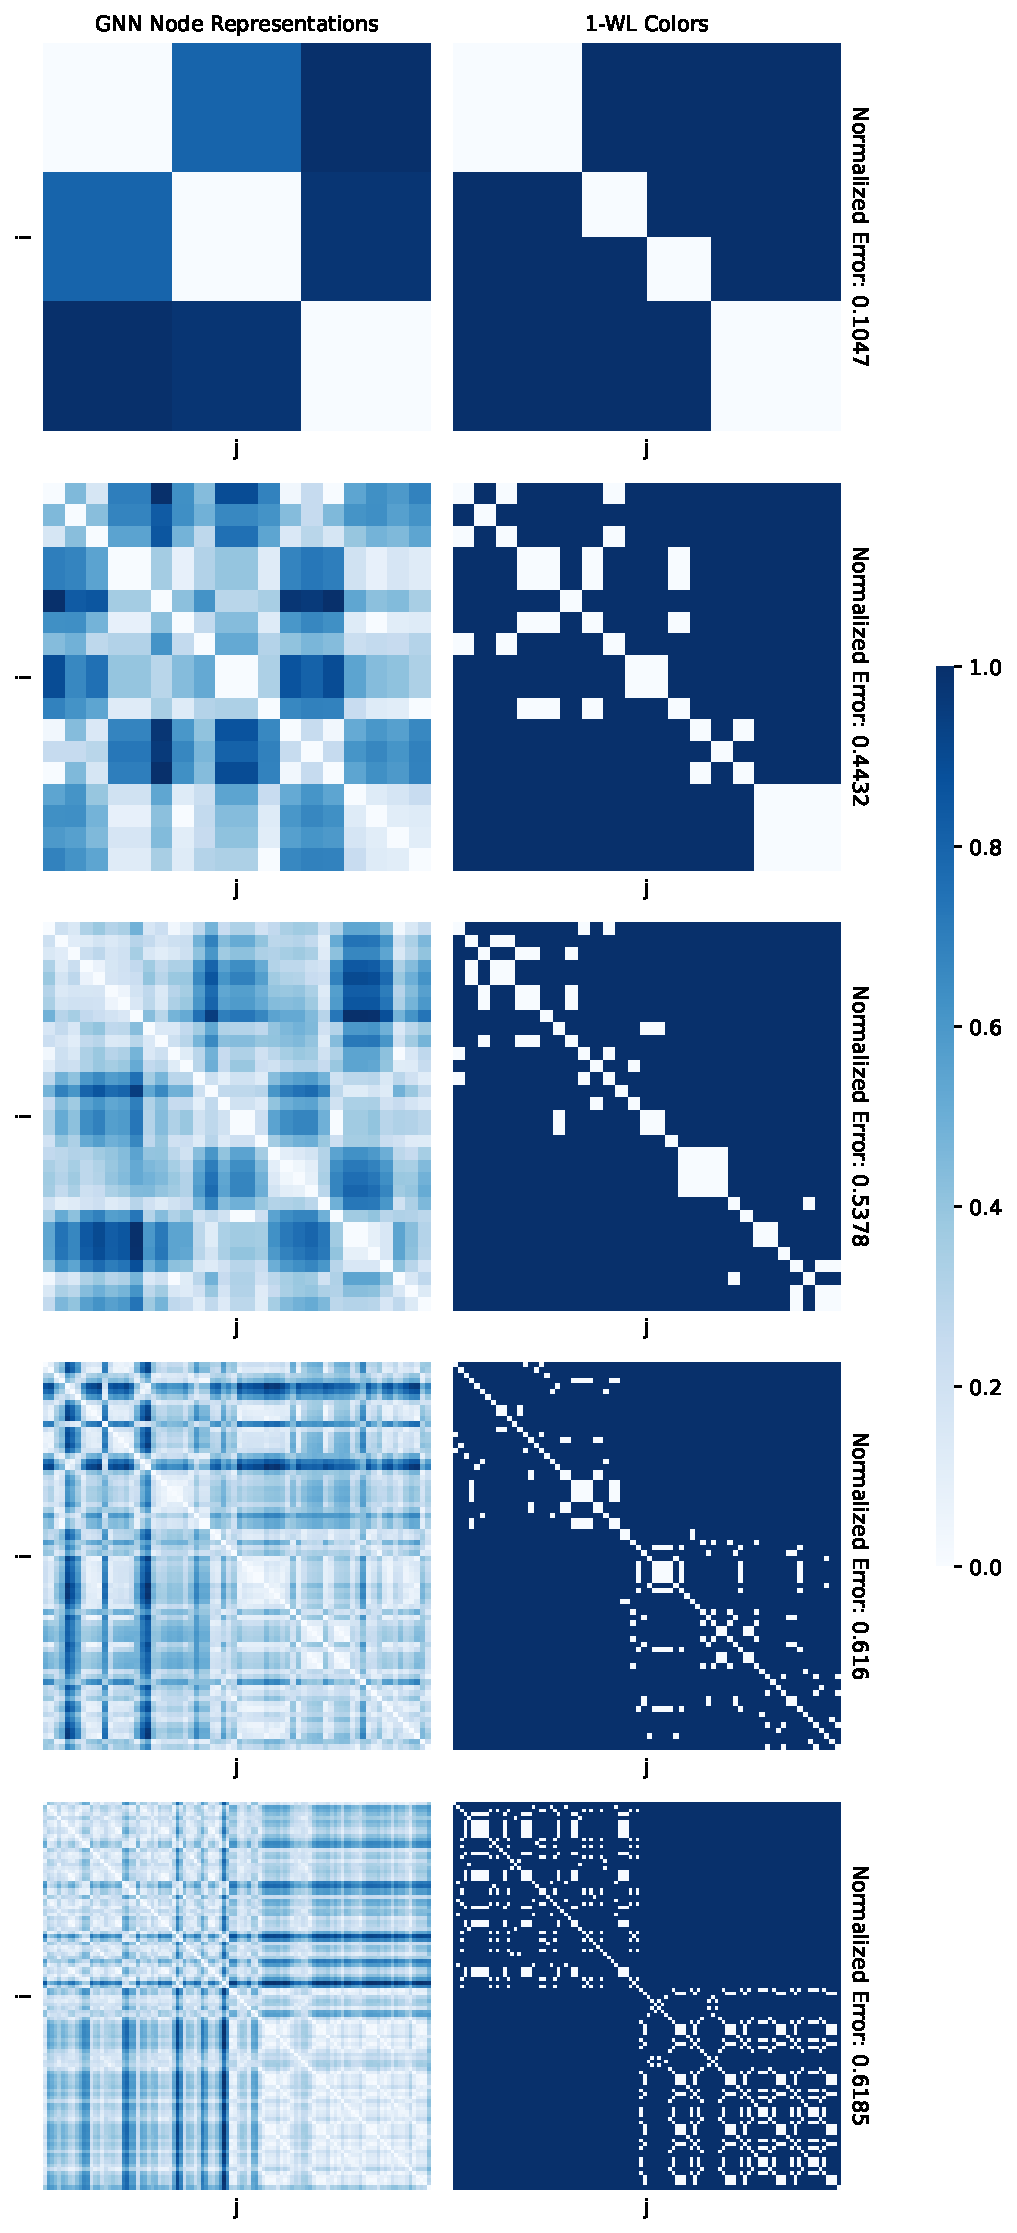
\includegraphics[width=\textwidth, right]{Figures/heatmaps_PROTEINS_1.pdf}
    \end{minipage}
    \hfill
    \caption{Visualizing the performance of the best performing \gnn on the \textsc{Proteins} dataset in approximating node colors computed by the \wl algorithm. The ten graphs shown are randomly sampled from the \gnn's test set. The average error for the entire test set is $0.49 \pm 0.26$.}
    \label{fig:gnn_approx_proteins}
\end{figure}
\clearpage

\subsubsection{\gnn Approximation Performance on the REDDIT-BINARY Dataset}
\begin{figure}[H]
    \centering
    \begin{minipage}[b]{0.45992852703\textwidth}
        \centering
        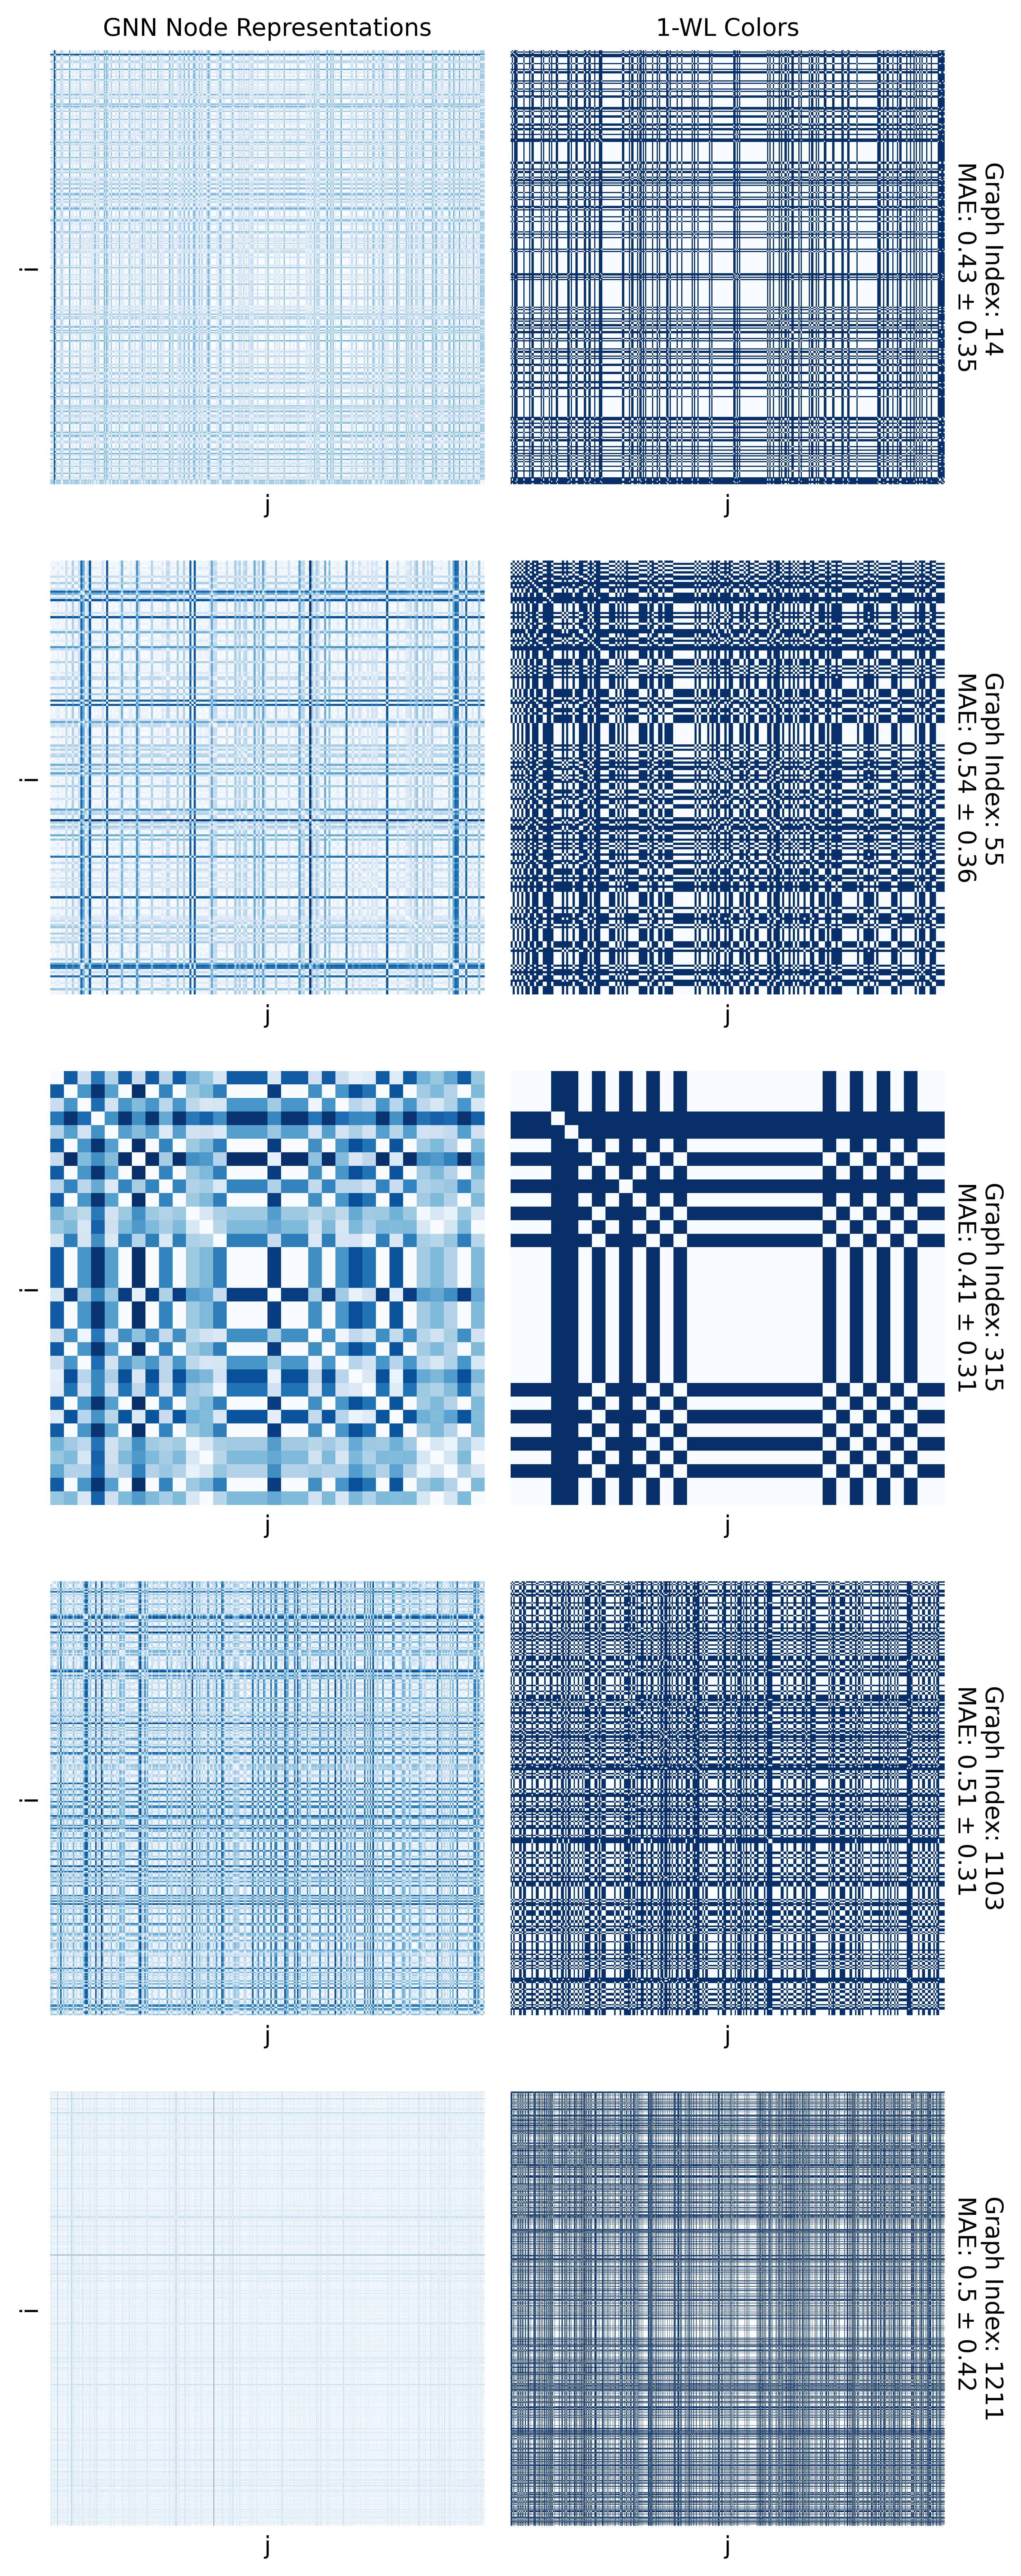
\includegraphics[width=\textwidth, left]{Figures/heatmaps_REDDIT-BINARY_0.png}
    \end{minipage}
    \hfill
    \begin{minipage}[b]{0.53007147296\textwidth}
        \includegraphics[width=\textwidth, right]{Figures/heatmaps_REDDIT-BINARY_1.png}
    \end{minipage}
    \hfill
    \caption{Visualizing the performance of the best performing \gnn on the \reddit dataset in approximating node colors computed by the \wl algorithm. The ten graphs shown are randomly sampled from the \gnn's test set. The average error for the entire test set is $0.48 \pm 0.32$.}
    \label{fig:gnn_approx_reddit}
\end{figure}
\clearpage
